%*********************************
%Format telah disesuaikan sesuai *
%Panduan penulisan               *
%Disertasi Dan Tesis ITS         *
%*********************************
%\documentclass[12pt, a4paper,twoside, bahasa]{report}

\documentclass[12pt, a4paper,twoside,opneany]{report}
\title{Buku Tesis}
% Jika pakai windows untuk run
%    pertama kali dan error.
% Mohon cek miktex console jika 
%    compiler latex nya menggunakan miktex.
%------------------------------
%%%%%%%%%%%%%%%%%%%%%%%%%%%%%%%%%%%%%%%%%%%%
% FILE KONFIGURASI TEMPLATE LATEX
%%%%%%%%%%%%%%%%%%%%%%%%%%%%%%%%%%%%%%%%%%%%

\usepackage[american]{babel}
\usepackage[utf8]{inputenc}
\usepackage{geometry}
\geometry{
	a4paper,
	left=40mm,
	top=35mm,
	right=30mm,
	bottom=30mm
}

% --- Paket Dasar & Algoritma ---
\usepackage{algorithm}
\usepackage{algpseudocode}
\renewcommand{\algorithmicrequire}{\textbf{Input:}}
\renewcommand{\algorithmicensure}{\textbf{Output:}}

% --- Paket Tampilan & Grafik ---
\usepackage{graphicx}
\usepackage{epsfig}
\usepackage{subcaption}
\usepackage{pdflscape}
\usepackage{lscape}
\usepackage{rotating}
\usepackage{adjustbox}
\usepackage{wrapfig}
\usepackage{float}
\usepackage{morefloats}
\usepackage{eso-pic}
\usepackage{pdfpages}

% --- Background Image ---
\newcommand\BackgroundIm{
	\put(0,0){
		\parbox[b][\paperheight]{\paperwidth}{%
			\vfill
			\centering
			\includegraphics[height=\paperheight,keepaspectratio]{./lib/background.png}%
			\vfill
}}}

% --- Paket Tabel ---
\usepackage{booktabs}
\setlength{\heavyrulewidth}{\lightrulewidth}
\usepackage{longtable}
\usepackage{multirow}
\usepackage{array,tabularx}
\usepackage[table,xcdraw]{xcolor}

% --- Paket Matematika & Simbol ---
\usepackage[fleqn]{amsmath}
\usepackage{amsfonts}
\usepackage{amssymb}
\usepackage{nccmath}
\usepackage{pifont}

\newcommand{\cmark}{\checkmark}
\newcommand{\xmark}{\ding{55}}
\newcommand{\specialcell}[1]{\begin{tabular}[c]{@{}c@{}}#1\end{tabular}}

% --- Paket Teks & Format ---
\usepackage{setspace}
\setstretch{1.5}
\linespread{1.5}
\usepackage{type1cm}
\usepackage{lettrine}
\usepackage{enumitem}
\usepackage{ulem}
\usepackage{titlesec}
\usepackage{multicol}
\usepackage{listings}
\usepackage{ragged2e}
\usepackage{lipsum}
\usepackage{hyphenat}
\usepackage{comment}
\usepackage{changepage}
\usepackage{afterpage}

% --- Referensi & Sitasi ---
\usepackage[round,authoryear]{natbib}
\usepackage{hyperref}
\hypersetup{hidelinks}
\usepackage[pageref]{backref}
\usepackage[nameinlink]{cleveref}

% --- Pengaturan Header & Footer ---
\usepackage{fancyhdr}
\usepackage{etoolbox}
\usepackage{url}
\usepackage{makeidx}
\makeindex

\fancyhf{}
\renewcommand{\headrulewidth}{0pt}
\pagestyle{fancy}
\fancyfoot[CE,CO]{\thepage}
\patchcmd{\chapter}{empty}{plain}{}{}

% --- Lingkungan / Environment Khusus ---
\newenvironment{FontCover}{\fontfamily{phv}\selectfont}{\par}

\newenvironment{Kondisi}
{\par\vspace{\abovedisplayskip}\noindent
	\tabularx{\columnwidth}{>{$}l<{$} @{${}:{}$} >{\raggedright\arraybackslash}X}}
{\endtabularx\par\vspace{\belowdisplayskip}}

\newenvironment{conditions}
{\par\vspace{\abovedisplayskip}\noindent
	\tabularx{\columnwidth}{>{$}l<{$} @{${}={}$} >{\raggedright\arraybackslash}X}}
{\endtabularx\par\vspace{\belowdisplayskip}}

% Fix titlesec bug
\makeatletter
\patchcmd{\ttlh@hang}{\parindent\z@}{\parindent\z@\leavevmode}{}{}
\patchcmd{\ttlh@hang}{\noindent}{}{}{}
\makeatother

% --- Pengaturan Section & Judul ---
\titleformat{\chapter}[display]{\bfseries\Large}{CHAPTER \centering\thechapter}{0ex}{\vspace{0ex}\centering}[\vspace{3ex}]
\titlespacing*{\chapter}{0pt}{-4ex}{0pt}
\titleformat{\section}{\bfseries\normalsize}{\MakeUppercase{\thesection}}{1ex}{}
\titleformat{\subsection}{\normalsize\bfseries}
\titleformat{\subsubsection}{\normalsize\bfseries}

\titlespacing{\section}{0pt}{0pt}{1ex}
\titlespacing{\subsection}{0pt}{0pt}{1ex}
\titlespacing{\subsubsection}{0pt}{0pt}{1ex}

% --- Caption Setup ---
\usepackage[labelfont=bf]{caption}
\captionsetup{labelfont=bf}
\captionsetup[figure]{font=small,skip=15pt}
\captionsetup[table]{font=small,skip=15pt}

\setlength{\floatsep}{8pt plus 2pt minus 2pt}
\setlength{\textfloatsep}{10pt plus 2pt minus 2pt}
\setlength{\intextsep}{10pt plus 2pt minus 2pt}

\DeclareCaptionLabelSeparator{none}{}
\captionsetup{labelsep=period}
\renewcommand{\figurename}{Figure}
\renewcommand{\tablename}{Table}
\renewcommand{\lstlistingname}{Code}

\setcounter{secnumdepth}{5}
\hyphenation{meng-gerak-kan mem-per-kenal-kan pe-ri-la-ku di-je-las-kan mem-bu-tuh-kan me-ne-rap-kan}

\def\kosong{
	\vspace*{\fill}
	\begin{center}\textit{This page is intentionally left blank}\end{center}
	\vfill
}
\patchcmd{\cleardoublepage}{\hbox{}}{\kosong}{}{}

\renewcommand*{\backreflastsep}{, }
\renewcommand*{\backreftwosep}{, }
\renewcommand*{\backref}[1]{}

% --- Bolean Variables ---
\newboolean{PembimbingDua}
\setboolean{PembimbingDua}{false}

\newboolean{bThesis}
\setboolean{bThesis}{true}

\newboolean{PembimbingTiga}
\setboolean{PembimbingTiga}{false}

\newboolean{PembimbingInternasional}
\setboolean{PembimbingInternasional}{false}

\newboolean{PengujiTiga}
\setboolean{PengujiTiga}{false}

\newboolean{PengujiEmpat}
\setboolean{PengujiEmpat}{false}

\newboolean{Nomenklatur}
\setboolean{Nomenklatur}{false}

\newboolean{bDoktor}
\setboolean{bDoktor}{false}

\newboolean{bMaster}
\setboolean{bMaster}{false}

\newboolean{JudulTesisEng}
\setboolean{JudulTesisEng}{false}

\renewcommand{\em}[1]{\textit{#1}}
\renewcommand{\emph}[1]{\textit{#1}}

% --- Definisi Perintah Identitas & Penguji ---
\newcommand{\Mahasiswa}[2]{
	\newcommand{\NamaMahasiswa}{#1}
	\newcommand{\NrpMahasiswa}{#2}
}

\newcommand{\PembimbingSatu}[2]{
	\newcommand{\PbSatu}{#1}
	\newcommand{\NipPbSatu}{#2}
}

\newcommand{\PembimbingDua}[2]{
	\setboolean{PembimbingDua}{true}
	\newcommand{\PbDua}{#1}
	\newcommand{\NipPbDua}{#2}
}

\newcommand{\PembimbingTiga}[2]{
	\setboolean{PembimbingTiga}{true}
	\newcommand{\PbTiga}{#1}
	\newcommand{\NipPbTiga}{#2}
}

\newcommand{\PengujiSatu}[2]{
	\newcommand{\PjSatu}{#1}
	\newcommand{\NipPjSatu}{#2}
}

\newcommand{\PengujiDua}[2]{
	\newcommand{\PjDua}{#1}
	\newcommand{\NipPjDua}{#2}
}

% FIXED: Menyesuaikan pembuatan variabel Penguji Tiga
\newcommand{\PengujiTiga}[2]{
	\setboolean{PengujiTiga}{true}
	\newcommand{\PjTiga}{#1}
	\newcommand{\NipPjTiga}{#2}
}

% FIXED: Mengaktifkan dan melengkapi variabel Penguji Empat
\newcommand{\PengujiEmpat}[2]{
	\setboolean{PengujiEmpat}{true}
	\newcommand{\PjEmpat}{#1}
	\newcommand{\NipPjEmpat}{#2}
}

\newcommand{\KaDep}[2]{
	\newcommand{\NmKaDep}{#1}
	\newcommand{\NipKaDep}{#2}
}

\newcommand{\CoverFooter}[1]{\newcommand{\bdk}{#1}}
\newcommand{\Judul}[1]{\newcommand{\JdTesis}{#1}}
\newcommand{\TanggalUjian}[1]{\newcommand{\TglUjian}{#1}}
\newcommand{\PeriodeWisuda}[1]{\newcommand{\PerWisuda}{#1}}
\newcommand{\Fakultas}[1]{\newcommand{\fak}{#1}}
\newcommand{\BeltFakultas}[1]{\newcommand{\bbelt}{#1}}
\newcommand{\Departemen}[1]{\newcommand{\Dep}{#1}}

\newcommand{\ggGelar}{xxxx}
\newcommand{\pPengesahan}{xxxxxxxx}

\newcommand{\Gelar}[1]{\renewcommand{\ggGelar}{#1}}
\newcommand{\tsss}{This dissertation is prepared to fulfill the requirements for obtaining\\the degree of}

\newcommand{\Disertasi}[1]{
	\renewcommand{\tsss}{This dissertation is prepared to fulfill the requirements for obtaining\\the degree of}
	\renewcommand{\pPengesahan}{STATEMENT OF APPROVAL}
	\renewcommand{\ggGelar}{#1}
	\setboolean{bMaster}{false}
	\setboolean{bThesis}{true}
}

\newcommand{\prop}{PROPOSAL DISERTASI}
\newcommand{\ProposalDisertasi}{
	\renewcommand{\prop}{PROPOSAL DISERTASI}
	\setboolean{bMaster}{false}
	\setboolean{bThesis}{false}
}

\newcommand{\Tesis}[1]{
	\renewcommand{\tsss}{Tesis disusun untuk memenuhi salah satu syarat memperoleh gelar}
	\renewcommand{\pPengesahan}{LEMBAR PENGESAHAN TESIS}
	\setboolean{bMaster}{true}
	\setboolean{bThesis}{true}
	\renewcommand{\ggGelar}{#1}
}

\newcommand{\ProposalTesis}{
	\setboolean{bMaster}{true}
	\renewcommand{\prop}{PROPOSAL TESIS}
	\setboolean{bThesis}{false}
}

\newcommand{\JudulEng}[1]{
	\setboolean{JudulTesisEng}{true}
	\newcommand{\JdTesisEng}{#1}
}

\newcommand{\Kode}[1]{\newcommand{\Kodekk}{#1}}
\newcommand{\TempatUjian}[1]{\newcommand{\bTempatUjian}{#1}}
\newcommand{\HariUjian}[1]{\newcommand{\bHariUjian}{#1}}

\newcommand{\DaftarRiwayatHidup}{
\addcontentsline{toc}{chapter}{AUTHOR'S BIOGRAPHY}
\titlespacing*{\chapter}{0pt}{0ex}{5ex}
\appendix
\chapter*{AUTHOR'S BIOGRAPHY}
%*********************************
%Gambar Foto 
	\begin{center}
		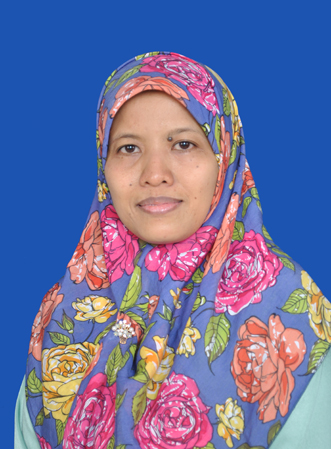
\includegraphics[height=0.2\textheight]{./ubah/Dini}
	\end{center}
%*********************************
\section*{Identity}
\begin{tabular}{p{3cm}cp{9cm}}
	%Masukan Identitas Disini.............
	Name  		  & :&
	Riandini \\
	Place of birth  & :&
		Jakarta\\
	Date of birth &:& 
		October $18^{th}$, 1977\\
	Address        &:& Depkes I, Jl. Husada I/79, Bekasi, 17412 \\
	%Identitas 1   &:&
	%	 Isi Identitas 1\\
	%Identitas 2   &:& 
	%	Isi Identitas 2\\
	%Identitas 3   &:&
	%	 Isi Identitas 3\\
	%Identitas 4   &:&
	%	 Isi Identitas 4\\
\end{tabular}

\section*{Education}
\begin{tabular}{p{3cm}cp{9cm}}
	2023-2027  	& :&
		Doctoral Degree (S3), Departement of Electrical Engineering, Faculty of Intelligent Electrical and Informatics Technology, Institut Teknologi Sepuluh Nopember\\
	&&\\
	2005-2007  & :&
		Master Degree (S2),Biomedical Engineering, University of Groningen\\
	&&\\
	1996-2001  & :&
		Bachelor Degree (S1), Department of Electrical Engineering, Institut Teknologi Bandung\\
	%&&\\
	%0000-0000  & :&
%		Pendidikan 1\\
	%&&\\
	%0000-0000  & :&
%		Pendidikan 2\\
%	&&\\
%	0000-0000  & :&
%		Pendidikan 3\\
\end{tabular}


\section*{Publications}

\begin{enumerate}
	\item Riandini, R., Purnama, K. E., Yuniarno, E. M., \& Purnomo, M. H. (2022, \large{bulan??}). Activation Function Selection for U-Net Multi-Structures Segmentation of End-Diastole and End-Systole Frames of Cine Cardiac MRI. In \textit{2022 IEEE Int. Conf. Imaging Systems and Techniques (IST)} (pp. ??). Taiwan (hybrid): IEEE.
	
	\item Riandini, Sardjono, T. A., Purnama, K. E., Yuniarno, E. M., \& Purnomo, M. H. (2023, June). A U-Net-Based System for Cine Cardiac Segmentation on MR Images: The Effect of Fuzzy Pooling Layer Type. In \textit{2023 IEEE Int. Symp. Medical Measurements and Applications (MeMeA)} \large{pp. ??}. Jeju, South Korea (hybrid): IEEE.
	
	\item Riandini, Yuniarno, E. M., Purnama, K. E., Aritsugi, M., \& Purnomo, M. H. (2025, July). Investigating Diverse Loss Functions for Myocardium Ring Segmentation in Cardiac Magnetic Resonance Images Using Fuzzy Pooling. \textit{Array}, 26, 100382, Elsevier. (Scopus Q1)
	
	\item Riandini, Setiadi, B., Yuniarno, E. M., Purnama, I. K. E., Aritsugi, M., \& Purnomo, M. H. (2026). MyoScarNet-RA: A Residual Attention Network for Myocardial Surface Area Quantification Based on Scar Segmentation. \textit{IEEE Access}, 14, 76722–76747. (Scopus Q1)
\end{enumerate}

\section*{Other Achievements and Research Experiences}
\begin{enumerate}
	\item International Grant from IEEE Engineering Projects in Community Service (EPICS), 2022, for the project titled: \textit{"\large{??}"}.
	\item National Book Chapter: \textit{Inovasi Teknologi Berbasis Kecerdasan Buatan dalam Bidang Kesehatan}. ISBN: 978-623-0275-84-5. Published in 2023 by Institut Teknologi Sepuluh Nopember, in collaboration with IEEE Industrial Electronics Society (IES) Indonesian Section and Deepublish.
	\item National Grant from Institut Teknologi Sepuluh Nopember (ITS), on the scheme of \textit{"\large{??}"}, 2025, for the research titled: \textit{"\large{??}"}.
	\item National Grant from Institut Teknologi Sepuluh Nopember (ITS), on the scheme of \textit{"\large{??}"}, 2025-2026, for the research titled: \textit{"\large{??}"}.
	\item Speaker in Webinar IEEE Industrial Application Society (IAS) - Indonesia Chapter, for the presentation titled: \textit{"AI dalam Kesehatan Jantung (Dari Diagnosis hingga Prediksi Risiko Penyakit)"}, July  $18^{th}$, 2026, 
\end{enumerate}

\cleardoublepage}
\newcommand{\DaftarPustaka}{\renewcommand{\bibname}{REFERENCES}
\addcontentsline{toc}{chapter}{\bibname}
\titlespacing*{\chapter}{0pt}{0ex}{5ex}
\appendix

%\bibliographystyle{IEEEtran}
%\bibliographystyle{harvard}
\bibliographystyle{plainnat}
\bibliography{IEEEabrv,./ubah/pustaka_dini}
\cleardoublepage}

\tolerance=9999
\emergencystretch=10pt
\hyphenpenalty=10000
\exhyphenpenalty=100



%************************************
% 1. JENIS BUKU
%    Pilih Salah Satu 
%************************************
%     \ProposalDisertasi
%     \ProposalTesis 
%     \Tesis{Magister Teknik (MT)}
%\Disertasi{Doktor (Dr)}
%***************************

%\ProposalDisertasi
%\ProposalTesis 
%\Tesis{Magister Teknik (MT)}
\Disertasi{Doctor (Dr)}


%*******************************
%2.  Tulislah Kode Yang Sesuai 
%*******************************
\Kode{Dissertation}
%\Kode{TESIS - EE184401}
%\Kode{Proposal Tesis}
%\Kode{Proposal Disertasi}
%*******************************

%*******************************
%  3. Judul Proposal, Tesis atau 
%     Disertasi 
%     dipilih Salah Satu 
%-------------------------------
% Tulislah Judul Dalam Bahasa Indonesia
\Judul{Cardiac Segmentation and Scar Quantification on CMR Images: A Deep Learning Approach Toward Myocardial Infarction (MI) Assessment}
% Tulislah Judul Dalam Bahasa Inggris
\JudulEng{Cardiac Segmentation and Scar Quantification on CMR Images: A Deep Learning Approach Toward Myocardial Infarction (MI) Assessment}
%************************************
% 4. Identitas Mahasiswa
% Format :\Mahasiswa{Nama}{Nrp}
%------------------------------------
\Mahasiswa{Riandini}{7022222013}
%************************************
% 5. Waktu Dan Ruang Ujian
%------------------------------------
%Tanggal Ujian 
\TanggalUjian{??? $??^{th}$, 2026}
% Perioda wisuda  
\PeriodeWisuda{} 
%Hari ujian dan Tempat Ujian 
\HariUjian{???}
\TempatUjian{B211}


%************************************
%6. Identitas Pembimbing 
%   Maximal Tiga Pembimbing
%   Format : \PembimbingXXX{Nama}{Nip}
%-----------------------------------
%\scalebox{.95}[1.0]{xxx}
\PembimbingSatu{Prof.Dr.Ir. Mauridhi Hery Purnomo, M.Eng.}{195809161986011001}
\PembimbingDua{Prof.Dr.I Ketut Eddy Purnama, S.T.,M.T.}{196907301995121001}
\PembimbingTiga{Dr. Eko Mulyanto Yuniarno, S.T.,M.T.}{196806011995121009}
%\PembimbingInternasional{Prof. Dr.Eng. Masayoshi Aritsugi}

%************************************
% 7. Identitas Penguji 
%     Maximal 4 penguji
%     Format : \PengujiXXX{Nama}{Nip}
%-------------------------
\PengujiSatu{Prof.Dr. Tri Arief Sardjono, S.T., M.T.}{197002121995121001}
\PengujiDua{Dr. Diah Puspito Wulandari, S.T., M.Sc}{198012192005012001}
%\PengujiTiga{Name ???}{??}
\PengujiTiga{Prof. Dr.Eng. Masayoshi Aritsugi}{}

%************************************
% 8. Identitas Fakultas ------------------------------------
\Fakultas{Faculty of Intelligent Electrical and Informatics Technology}
\BeltFakultas{BeltFte}
%************************************
% 9. Identitas Departement
%-----------------------------------
\Departemen{Electrical Engineering }

\KaDep{Ronny Mardiyanto, S.T., M.T., Ph.D.}{198101182003121003}
%***********************************
% 10. Footer Identitas Program Studi 
%  Pada Cover
%----------------------------------
\CoverFooter{\normalsize
DOCTORAL PROGRAM\\
	DEPARTEMENT OF ELECTRICAL ENGINEERING\\
	FACULTY OF INTELLIGENT ELECTRICAL \& INFORMATICS TECHNOLOGY\\
	INSTITUT TEKNOLOGI SEPULUH NOPEMBER\\
	SURABAYA\\
	2026}

%**********************************
%File Penting Yang Dapat di Edit:
%**********************************
%Abstrak :
%        ->\ubah\abstrak.tex
%Abstrak Bhs Inggris :
%        ->\ubah\abstrakEng.tex
%Kata Penggantar :
%        ->\ubah\pengantar.tex 
%Nomenklatur :
%        ->\ubah\Nomenklatur.tex
%Database Daftar Pustaka
%        ->\ubah\pustaka.bib
%DaftarRiwayatHidup 
%        ->\ubah\DaftarRiwayatHidup.tex
%----------------------------------
%**********************************
%Dokumen Utama
%----------------------------------
\begin{document}
	
	\input{./lib/Tataletak.tex}
	
	\begin{spacing}{1.5}
		
		\chapter{INTRODUCTION}
\label{chap:1}

\section{Background}
\label{sec:background}

Cardiovascular disease (CVD) remains the leading cause of mortality and
morbidity worldwide \citep{WHO2021,Tsao2022}, with coronary heart disease (CHD) accounting for a
substantial proportion of cardiovascular-related deaths. Among the
various manifestations of CHD, myocardial infarction (MI) represents one
of the most critical cardiovascular conditions because prolonged
interruption of coronary blood flow causes irreversible myocardial
injury, leading to myocardial necrosis, fibrotic scar formation,
ventricular remodeling, impaired cardiac function, and increased
mortality. Consequently, accurate assessment of myocardial infarction is
essential for determining disease severity, therapeutic planning, risk
stratification, and long-term prognosis \citep{Thygesen2019}.

In Indonesia, cardiovascular disease also represents a major healthcare
challenge. According to the Indonesian Ministry of Health \citep{Kemenkes2021},
cardiovascular disease accounts for one of the largest healthcare
expenditures under the National Health Insurance (JKN) program. This
increasing disease burden highlights the need for reliable, objective,
and efficient technologies that can support clinical decision-making
while improving the consistency and reproducibility of cardiac image
analysis.

Cardiac Magnetic Resonance (CMR) has become the reference imaging
modality for myocardial infarction assessment because it provides
excellent soft-tissue contrast, high spatial resolution, and
comprehensive visualization of both cardiac anatomy and myocardial
pathology without exposing patients to ionizing radiation \citep{Kim2000,Kramer2020}. Different CMR sequences provide
complementary diagnostic information. Cine CMR enables accurate
visualization of cardiac structures and ventricular function, whereas
Late Gadolinium Enhancement (LGE) imaging accurately identifies
infarcted and fibrotic myocardial tissue. The combination of these
imaging sequences enables comprehensive assessment of myocardial
infarction from both anatomical and pathological perspectives. The
overall workflow of the proposed framework developed in this
dissertation is illustrated in Figure~\ref{fig:ch1-proposed}. The framework integrates cardiac structure segmentation, reliable myocardium
segmentation, myocardial scar segmentation, and quantitative scar
assessment to support comprehensive myocardial infarction assessment.


\begin{figure}[htbp]
	\centering
	\fbox{\parbox{0.82\textwidth}{\centering Insert Figure 1.1 here}}
	\caption{Overview of the Proposed Deep Learning Framework for CMR Image Analysis for Myocardial Infarction Assessment}
	\label{fig:ch1-proposed}
\end{figure}

Reliable myocardial infarction assessment cannot be achieved directly
from scar segmentation alone. Since myocardial scar is anatomically
confined within the myocardium, accurate cardiac structure segmentation
provides the anatomical foundation for subsequent pathological analysis.
Reliable myocardium segmentation subsequently defines the region of
interest for scar localization, while accurate scar segmentation enables
quantitative assessment of myocardial scar extent. Because these stages
are sequentially connected, errors introduced during earlier analyses
may propagate to subsequent stages and reduce the reliability of the
final assessment.

Despite the superior capability of CMR, image interpretation in routine
clinical practice remains largely dependent on manual image analysis
performed by experienced cardiologists and radiologists. Manual analysis
is time-consuming and susceptible to intra-observer and inter-observer
variability, particularly when myocardial boundaries are indistinct or
scar tissue exhibits heterogeneous signal intensity. These limitations
motivate the development of automated image analysis methods capable of
providing more objective, consistent, and efficient myocardial
infarction assessment.

Recent advances in deep learning have significantly improved medical
image segmentation, including CMR image analysis. Encoder-decoder
architectures, particularly U-Net and its variants, have demonstrated
excellent performance for cardiac structure segmentation, whereas
residual learning, attention mechanisms, and improved improved learning
strategies have further enhanced segmentation accuracy across various
medical imaging applications \citep{Ronneberger2015,He2016,Oktay2018}. Nevertheless, several methodological challenges
remain.

First, preservation of fine anatomical information during cardiac
structure segmentation remains challenging because repeated
down-sampling operations may reduce spatial resolution and boundary
continuity. Second, reliable myocardium segmentation is still affected
by class imbalance and ambiguous myocardial boundaries, requiring
effective learning strategies during network training. Third, myocardial
scar segmentation remains difficult because scar tissue generally
occupies only a small portion of the myocardium while exhibiting
heterogeneous signal intensity and irregular morphology. Finally,
although numerous studies have reported improvements in individual image
analysis tasks, these studies generally investigate each task
independently rather than integrating them into a unified framework for
myocardial infarction assessment.

The research gaps identified from previous studies are illustrated in
Figure~\ref{fig:ch1-fishbone} and summarized in Table~\ref{tab:ch1-tab1_1}. Although considerable progress has been achieved in individual image analysis
tasks, these studies generally address each component independently
rather than integrating them into a unified framework for myocardial
infarction assessment.

\begin{figure}[htbp]
	\centering
	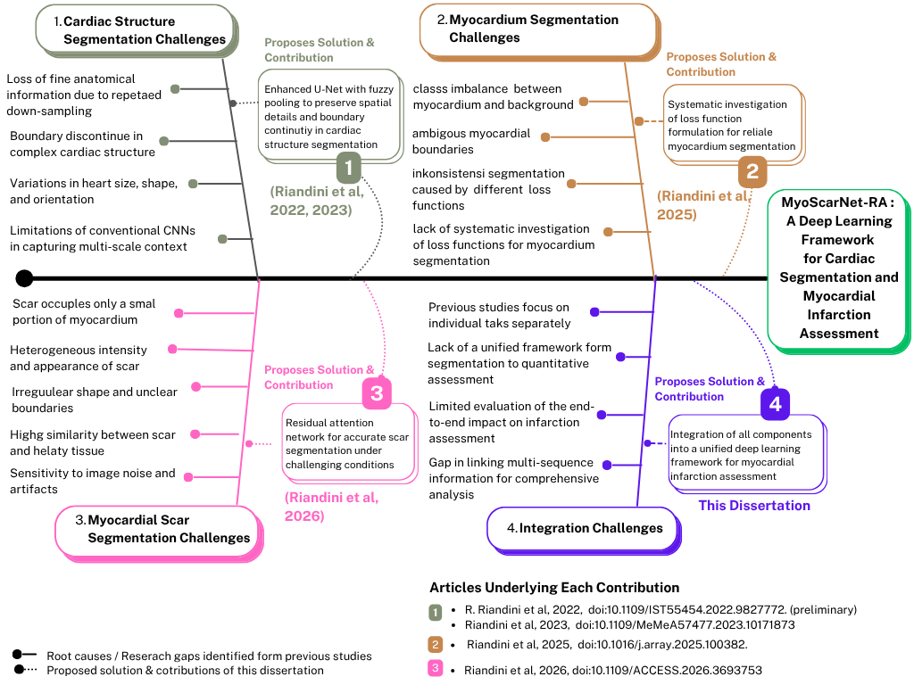
\includegraphics[width=0.86\textwidth]{bab1/ch1-fishbone.png}
	\caption{Fishbone analysis of research challenges in CMR analysis for MI assessment and the proposed solutions with corresponding contributions of this dissertation}
	\label{fig:ch1-fishbone}
\end{figure}

Table 1.1. Research Gap Analysis and Positioning of the Proposed
Dissertation

\begin{longtable}[]{@{}
		>{\raggedright\arraybackslash}p{(\columnwidth - 4\tabcolsep) * \real{0.2444}}
		>{\raggedright\arraybackslash}p{(\columnwidth - 4\tabcolsep) * \real{0.2782}}
		>{\raggedright\arraybackslash}p{(\columnwidth - 4\tabcolsep) * \real{0.4774}}@{}}
	\toprule
	\textbf{Previous Studies} & \textbf{Remaining Limitation} & \textbf{Position of This Dissertation} \\
	\midrule
	\endhead
	
	Cardiac structure segmentation & Focused on anatomical segmentation & Enhanced U-Net with fuzzy pooling \\
	Myocardium segmentation & Investigated independently & Reliable myocardium segmentation through loss function investigation \\
	Myocardial scar segmentation & Focused only on scar segmentation & Residual attention-based scar segmentation with quantitative assessment \\
	Individual image analysis tasks & Conducted separately & Integrated deep learning framework for myocardial infarction assessment \\
	\bottomrule
	\label{tab:ch1-tab1_1}
\end{longtable}

Motivated by these challenges, this dissertation develops an integrated
deep learning framework for CMR image analysis. The proposed framework
consists of four complementary stages: \textbf{(1)} cardiac structure
segmentation using an enhanced U-Net incorporating fuzzy pooling,
\textbf{(2)} reliable myocardium segmentation through systematic
investigation of different loss function formulations, \textbf{(3)}
residual attention-based myocardial scar segmentation followed by
quantitative scar assessment, and \textbf{(4)} integration of these
methodological developments into a unified framework for automated
myocardial infarction assessment. Through this integrated approach, the
dissertation establishes a coherent methodological pathway from
anatomical cardiac representation to quantitative myocardial scar
assessment, providing a comprehensive approach for CMR image analysis.

\section{Research Problems}
\label{sec:research-problems}

Based on the background presented in the previous section, several
research problems remain to be addressed in CMR image analysis for
myocardial infarction assessment. These research problems are formulated
as follows.

\begin{enumerate}
	\def\labelenumi{\arabic{enumi}.}
	\item
	How can cardiac structure segmentation be improved while preserving
	important anatomical information from CMR images?
	\item
	How can reliable myocardium segmentation be achieved under class
	imbalance and ambiguous myocardial boundaries?
	\item
	How can myocardial scar be accurately segmented and quantitatively
	assessed from CMR images?
\end{enumerate}

How can cardiac structure segmentation, reliable myocardium
segmentation, myocardial scar segmentation, and quantitative scar
assessment be integrated into a unified deep learning framework for
myocardial infarction assessment?

\section{Research Objectives}
\label{sec:research-objectives}

The main objective of this dissertation is to develop a deep
learning-based framework for CMR image analysis for myocardial
infarction assessment.

To achieve this objective, the following specific objectives are
established.

\begin{enumerate}
	\def\labelenumi{\arabic{enumi}.}
	\item
	To develop an enhanced U-Net incorporating fuzzy pooling for accurate
	cardiac structure segmentation from CMR images.
	\item
	To investigate different loss function formulations in order to obtain
	reliable myocardium segmentation.
	\item
	To develop a residual attention-based framework for myocardial scar
	segmentation and quantitative scar assessment.
	\item
	To integrate the proposed methods into a unified deep learning
	framework for myocardial infarction assessment.
\end{enumerate}

\section{Scientific Contributions}
\label{sec:scientific-contributions}

This dissertation makes four principal scientific contributions to the
development of deep learning methods for CMR image analysis for
myocardial infarction assessment.

\textbf{Contribution 1}

An enhanced U-Net incorporating fuzzy pooling is developed to improve
cardiac structure segmentation while preserving important anatomical
information from CMR images.

\textbf{Contribution 2}

A systematic investigation of different loss function formulations is
conducted to identify an effective approach for reliable myocardium
segmentation under class imbalance and ambiguous myocardial boundaries.
The investigation identified the combination of Cross-Entropy and
Lovász-Softmax as the most effective loss formulation among the
evaluated loss functions.

\textbf{Contribution 3}

A residual attention-based framework is developed for myocardial scar
segmentation and quantitative scar assessment, enabling automatic
estimation of myocardial scar area from CMR images.

\textbf{Contribution 4}

An integrated deep learning framework that supports objective myocardial
infarction assessment by combining cardiac structure segmentation,
myocardium segmentation, myocardial scar segmentation, and quantitative
scar area assessment.

\section{Research Novelty}
\label{sec:research-novelty}

Previous studies have generally investigated cardiac structure
segmentation, myocardium segmentation, myocardial scar segmentation, and
quantitative scar assessment as separate research problems. In contrast,
this dissertation develops a unified deep learning framework that
integrates these methodological components into a coherent workflow for
myocardial infarction assessment using cardiac magnetic resonance (CMR)
images.

\textbf{The principal novelties of this dissertation are summarized as
	follows.}

\begin{enumerate}
	\def\labelenumi{\arabic{enumi}.}
	\item
	\textbf{Development of an enhanced U-Net architecture incorporating
		fuzzy pooling} for cardiac structure segmentation from cine CMR
	images.
	\item
	\textbf{Systematic investigation of multiple loss function
		formulations, including the proposed CrossLov loss}, for myocardium
	segmentation under identical experimental conditions.
	\item
	\textbf{Development of MyoScarNet-RA}, a residual attention-based
	framework for myocardial scar segmentation and quantitative scar area
	assessment using multi-sequence CMR images.
	\item
	\textbf{Integration of the above methodological developments into a
		unified deep learning framework} for myocardial infarction
	assessment.''
\end{enumerate}

\section{Research Significance}
\label{sec:research-significance}

The outcomes of this dissertation are expected to provide academic,
clinical, and practical significance in the field of CMR image analysis
for myocardial infarction assessment.

\textbf{Scientific Significance}

This dissertation contributes to the advancement of deep learning
research in CMR image analysis by providing an integrated framework that
combines cardiac structure segmentation, reliable myocardium
segmentation, myocardial scar segmentation, and quantitative scar
assessment. The proposed framework also provides a systematic reference
for future studies involving automated myocardial infarction assessment
using CMR images.

\textbf{Clinical Significance}

The proposed framework is expected to support more objective,
consistent, and efficient analysis of CMR images. By reducing dependence
on manual image interpretation, the proposed methods may assist
clinicians in evaluating myocardial infarction through more reliable
assessment of cardiac structures and myocardial scar characteristics.

\textbf{Practical Significance}

The proposed framework may serve as a foundation for developing
computer-aided CMR image analysis systems. In addition, the
methodological developments presented in this dissertation may
facilitate future research on automated cardiac image analysis and
support the development of intelligent clinical decision-support
systems.

\section{Research Scope and Limitations}
\label{sec:research-scope}

The scope and limitations of this dissertation are defined to establish
the research boundaries and clarify the applicability of the proposed
framework. The scope and limitations of this study are summarized as
follows.

\begin{enumerate}
	\def\labelenumi{\arabic{enumi}.}
	\item
	This dissertation focuses exclusively on myocardial infarction
	assessment using CMR images.
	\item
	Cardiac structure segmentation is developed and evaluated using the
	Automated Cardiac Diagnosis Challenge (ACDC) dataset, whereas
	myocardial scar segmentation and quantitative scar assessment are
	performed using the Myocardial Pathology Segmentation (MyoPS2020)
	dataset.
	\item
	The investigated cardiac structures are limited to the left ventricle,
	right ventricle, and myocardium.
	\item
	The proposed framework consists of four sequential image analysis
	stages: cardiac structure segmentation, reliable myocardium
	segmentation, myocardial scar segmentation, and quantitative scar
	assessment.
	\item
	This study focuses on automated CMR image analysis and does not
	include clinical diagnosis, prognosis prediction, treatment
	recommendation, or longitudinal patient monitoring.
	\item
	Performance evaluation is limited to image segmentation accuracy,
	quantitative scar measurement, and statistical agreement using the
	evaluation metrics presented in this dissertation.
\end{enumerate}

\section{Dissertation Organization}
\label{sec:dissertation-organization}

This dissertation is organized into seven chapters.

\textbf{Chapter I}, entitled "Introduction" introduces the research background, research
problems, research objectives, scientific contributions, research
significance, research novelty, research scope and limitations, and the
overall organization of the dissertation.

\textbf{Chapter II}, entitled "Literature Review" reviews the theoretical background and related studies on CMR imaging, deep learning, cardiac structure segmentation, myocardium segmentation, myocardial scar segmentation, quantitative scar assessment, and previous studies relevant to this dissertation.

\textbf{Chapter III}, entitled "Research Methodology" presents the overall research methodology, including research datasets, dataset preparation, cardiac structure segmentation, anatomical myocardium prior generation, myocardial scar segmentation, quantitative scar assessment, performance evaluation, and agreement analysis. 

\textbf{Chapter IV}, entitled "Cardiac Structure Segmentation Using an Enhanced U-Net with Fuzzy Pooling," presents the development and evaluation of the proposed enhanced U-Net for cardiac structure segmentation.

\textbf{Chapter V}, entitled "Loss Function Investigation for Reliable Myocardium Segmentation," presents a systematic investigation of different loss function formulations to identify the most effective approach for reliable myocardium segmentation.

\textbf{Chapter VI}, entitled "Residual Attention-Based Myocardial Scar Segmentation and Quantitative Scar Assessment," presents the proposed residual attention-based framework for myocardial scar segmentation and quantitative scar assessment.

\textbf{Chapter VII}, entitled "General Conclusions and Future Work," summarizes the principal findings of the dissertation, highlights the overall scientific contributions, and discusses recommendations for future research. 

		%\cleardoublepage
		\clearpage
		
		\chapter{LITERATURE REVIEW}
\label{chap:2}

\section{Myocardial Infarction}
\label{sec:mi}

Myocardial infarction (MI), commonly known as a heart attack, is one of the leading causes of morbidity and mortality worldwide. It occurs when blood flow through a coronary artery is partially or completely blocked, resulting in prolonged oxygen deprivation of the heart muscle. If blood supply is not restored promptly, irreversible damage to the myocardium occurs, leading to the formation of non-contractile scar tissue and permanent impairment of cardiac function \citep{Thygesen2019}.

Following myocardial infarction, the damaged myocardium undergoes a healing process in which necrotic tissue is gradually replaced by fibrotic scar tissue. Unlike healthy myocardium, scar tissue has little or no contractile capability, reducing the pumping efficiency of the left ventricle. Extensive myocardial scarring has been associated with ventricular remodeling, heart failure, life-threatening arrhythmias, and an increased risk of sudden cardiac death \citep{Thygesen2019,Ibanez2018}.

\begin{figure}[htbp]
	\centering
	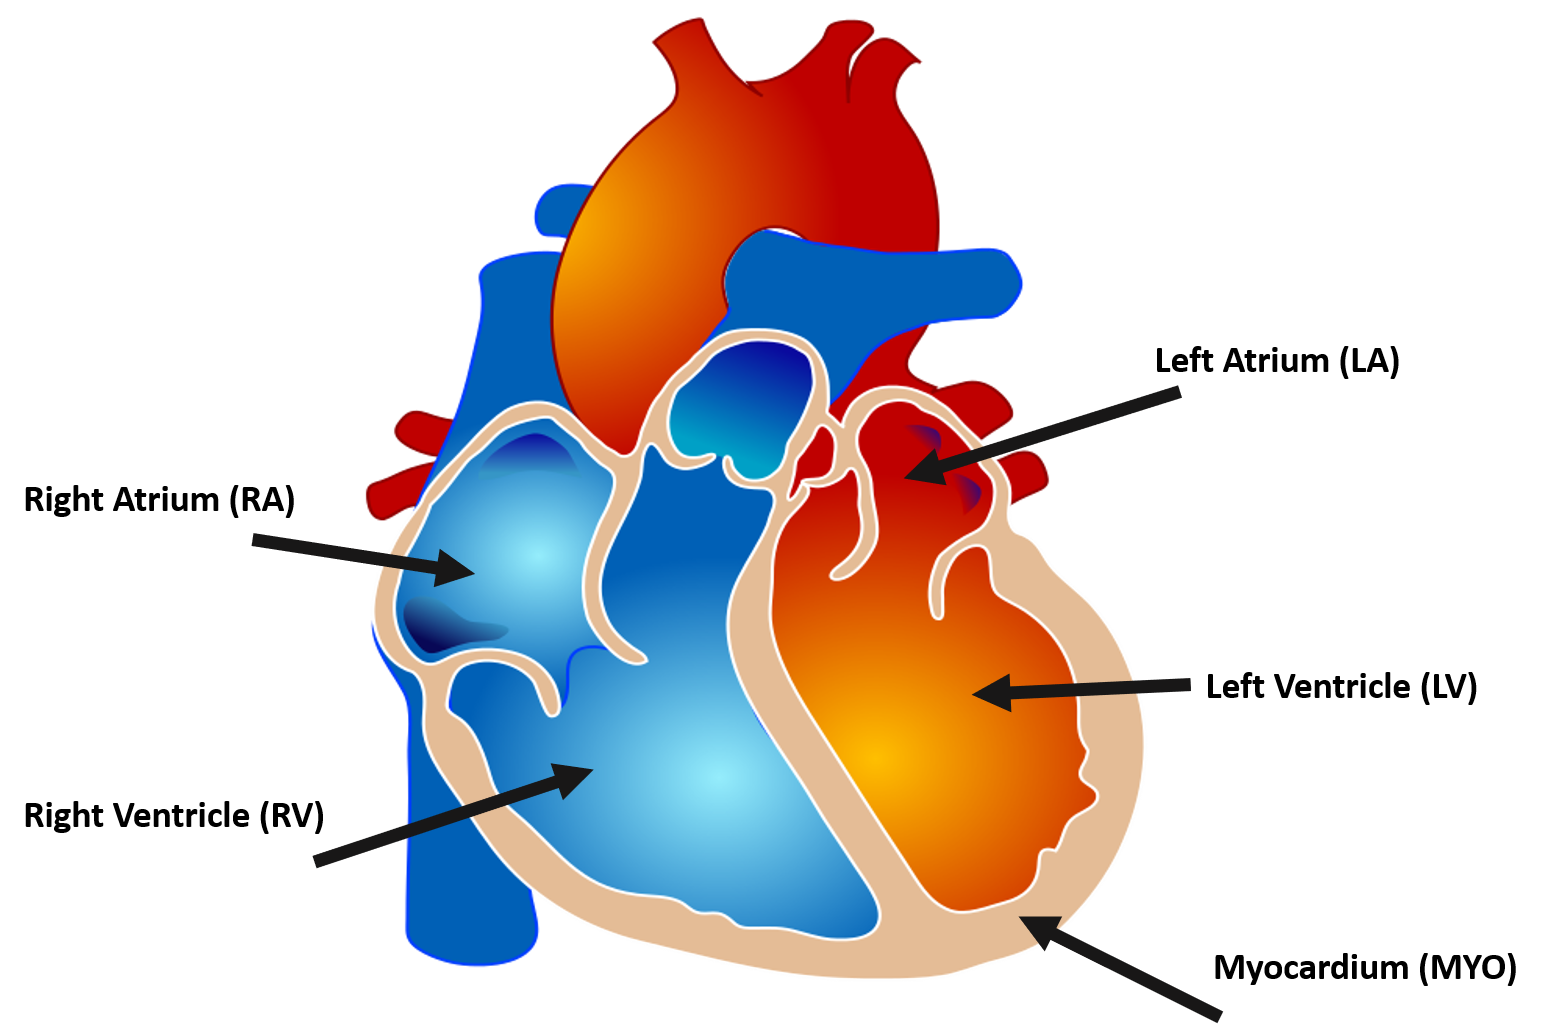
\includegraphics[width=0.86\textwidth]{bab2/ch2-heart-anatomy.png}
	\caption{Anatomy of the human heart \citep{Shade2013}}
	\label{fig:ch2-heart-anatomy}
\end{figure}

Figure~\ref{fig:ch2-heart-anatomy} illustrates the basic anatomy of the heart, including the left ventricle, right ventricle, atria, and myocardium. Among these structures, the myocardium is the primary region affected by myocardial infarction and therefore becomes the main focus of this dissertation.

\begin{figure}[htbp]
	\centering
	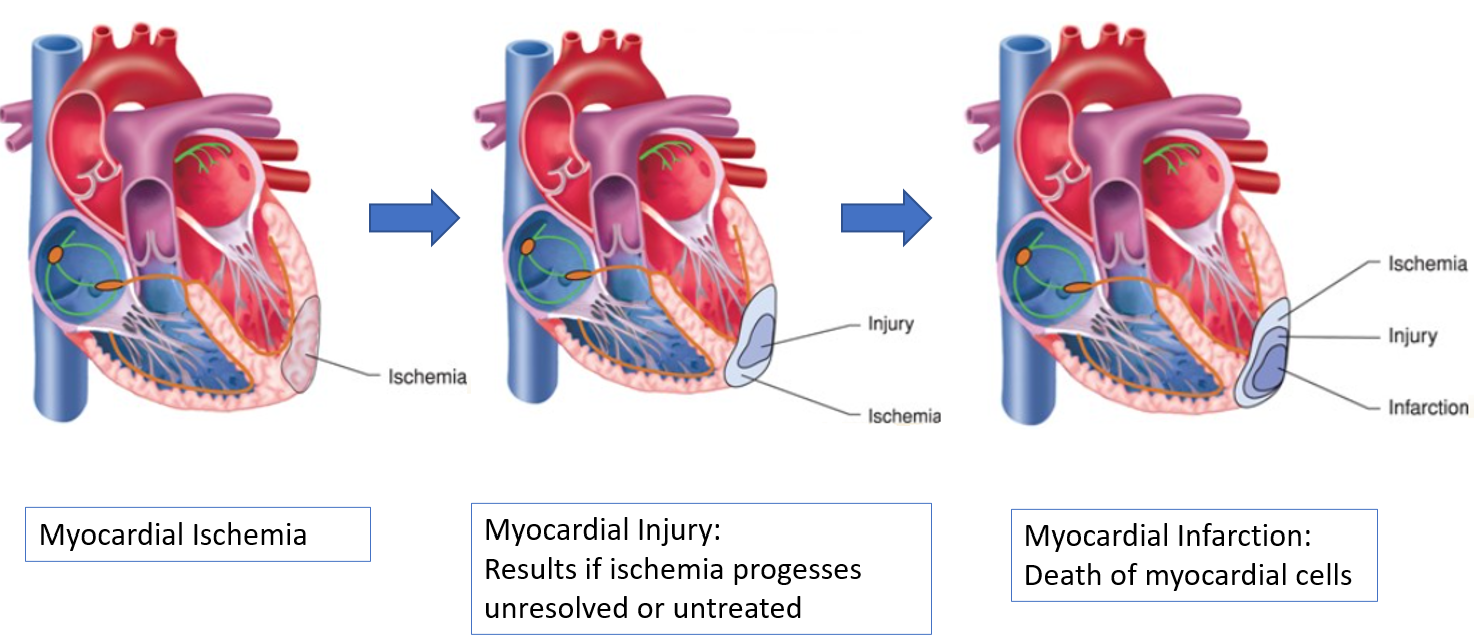
\includegraphics[width=0.86\textwidth]{bab2/ch2-mi-development.png}
	\caption{Development of myocardial infarction following prolonged coronary artery obstruction \citep{Shade2013}}
	\label{fig:ch2-mi-development}
\end{figure}

As illustrated in Figure~\ref{fig:ch2-mi-development}, prolonged interruption of blood supply causes myocardial cells to lose oxygen and nutrients, eventually resulting in irreversible tissue injury. During the healing process, the damaged myocardium is replaced by fibrotic scar tissue, which permanently alters the mechanical function of the heart.

\begin{figure}[htbp]
	\centering
	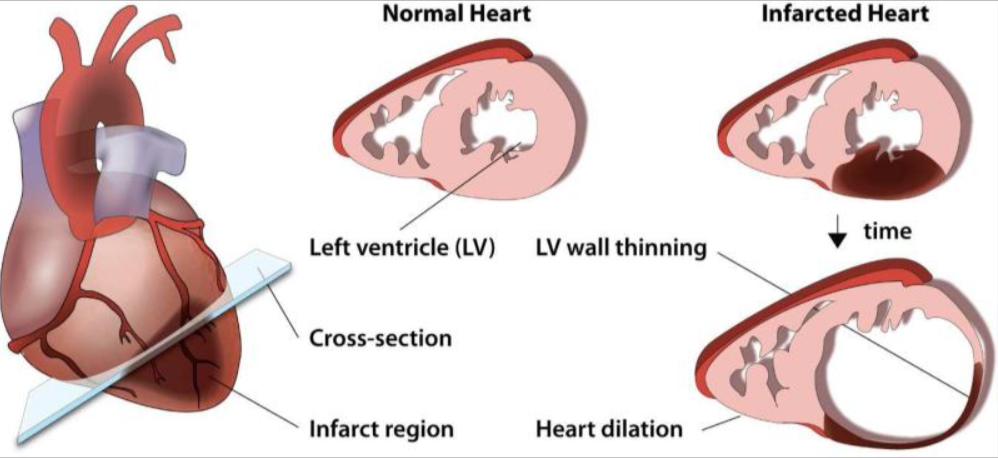
\includegraphics[width=0.86\textwidth]{bab2/ch2-healthy-infarcted.png}
	\caption{Comparison of healthy and infarcted myocardium \citep{Awada2016}}
	\label{fig:ch2-healthy-infarcted}
\end{figure}

The extent and location of myocardial scar are closely related to cardiac function and clinical outcome. Consequently, accurate assessment of myocardial scar has become an essential component in the diagnosis, treatment planning, and follow-up of patients with myocardial infarction. Reliable scar quantification provides valuable information for evaluating infarct severity, predicting functional recovery, and supporting therapeutic decision-making \citep{Kim2000,Ibanez2018}.

Although several imaging modalities are available for cardiac assessment, each has different strengths and limitations in visualizing myocardial tissue. Among these modalities, CMR has emerged as the reference standard because it enables comprehensive evaluation of cardiac anatomy, ventricular function, and myocardial tissue characteristics within a single examination. Therefore, the following section reviews the principles and clinical advantages of CMR for myocardial infarction assessment.

\section{Cardiac Magnetic Resonance Imaging}
\label{sec:cmr}

Cardiac Magnetic Resonance (CMR) has become one of the most important imaging modalities for the evaluation of cardiovascular diseases because it provides comprehensive information on cardiac anatomy, ventricular function, tissue characterization, and myocardial viability without exposing patients to ionizing radiation. Compared with echocardiography, computed tomography (CT), and nuclear imaging, CMR offers superior soft tissue contrast and high spatial resolution, making it particularly suitable for myocardial infarction assessment \citep{Kramer2020,Pennell2010}.

CMR examinations can be performed using different imaging sequences, each providing complementary clinical information. Among these, cine CMR is widely used to evaluate cardiac morphology and ventricular function, whereas Late Gadolinium Enhancement (LGE) imaging is considered the clinical reference for detecting myocardial scar. The combination of these imaging sequences enables both functional and structural assessment of the myocardium within a single examination \citep{Kramer2020}.

\begin{figure}[htbp]
	\centering
	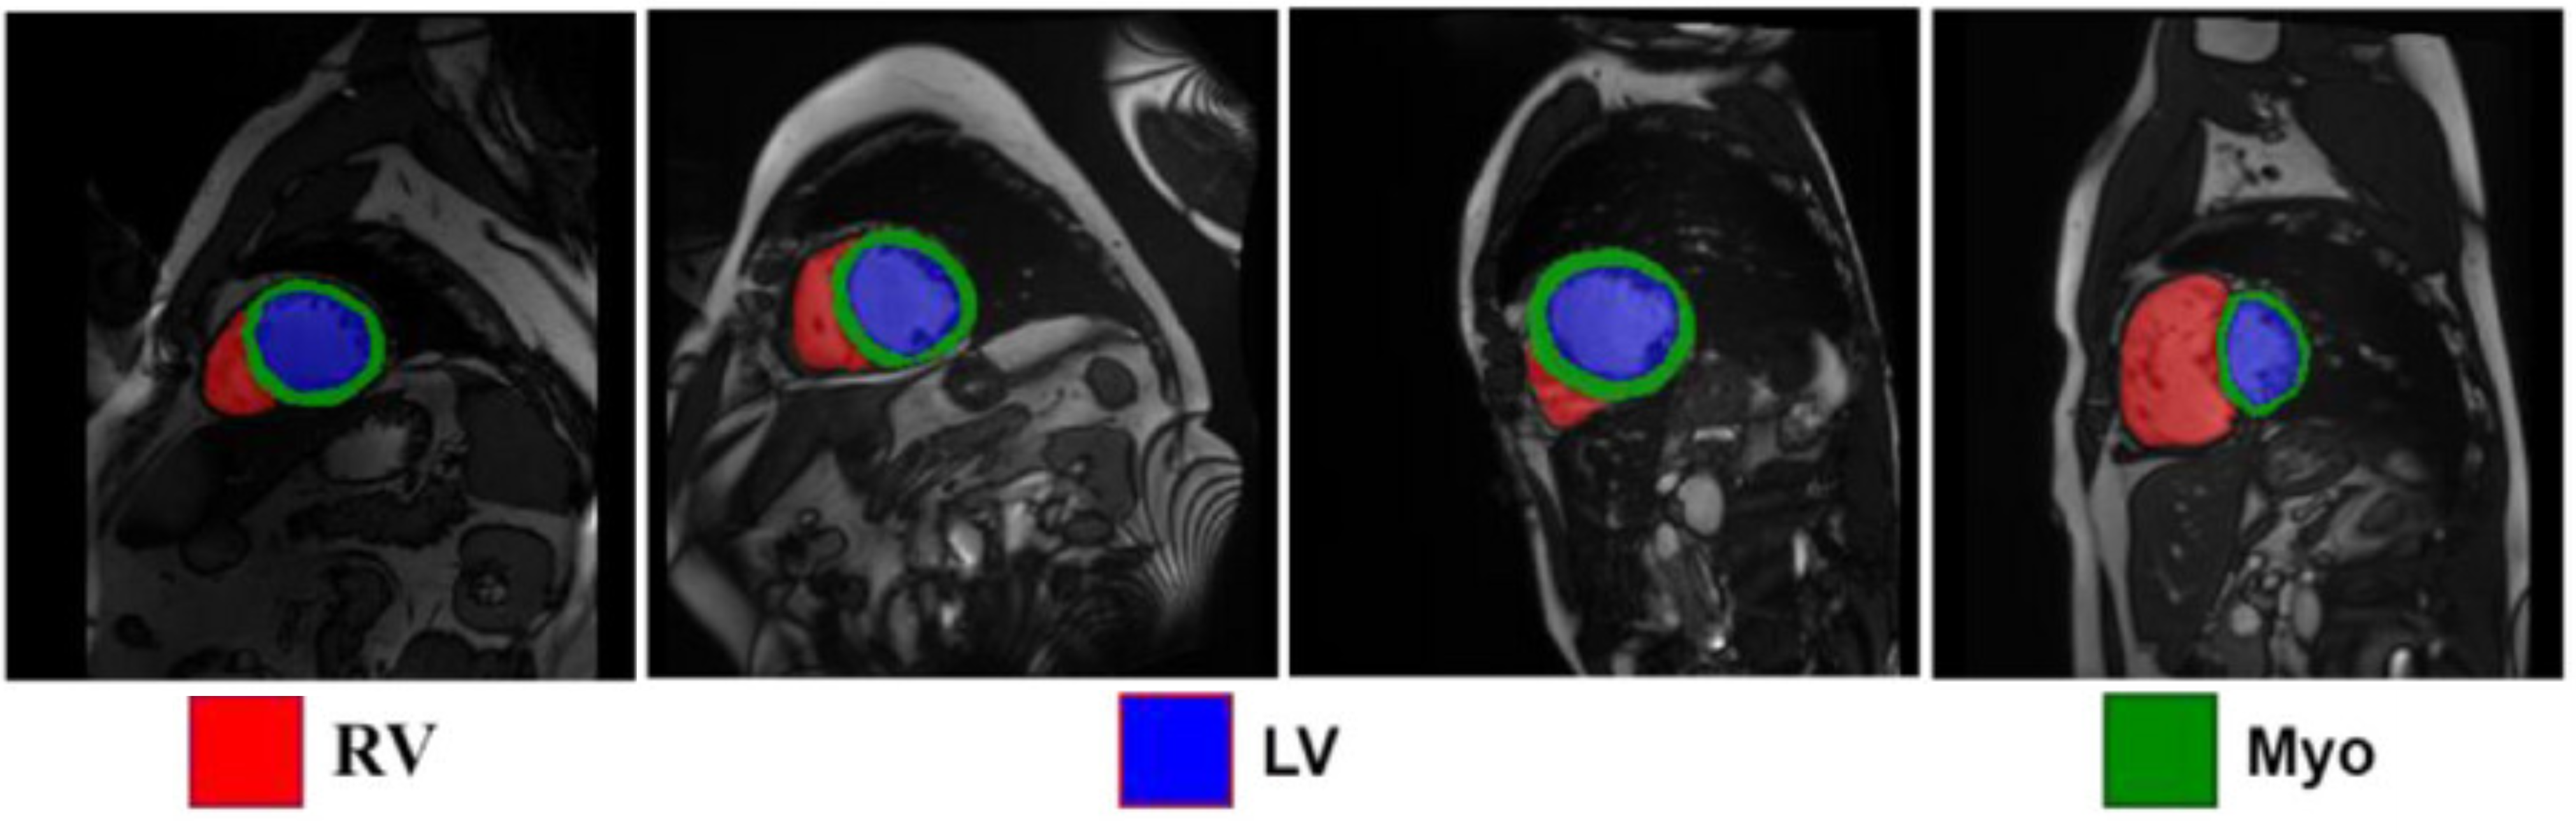
\includegraphics[width=0.86\textwidth]{bab2/ch2-cmr-sequences.png}
	\caption{Representative CMR imaging sequences used for myocardial infarction assessment \citep{Xie2024}}
	\label{fig:ch2-cmr-sequences}
\end{figure}

Figure~\ref{fig:ch2-cmr-sequences} illustrates the complementary information provided by different CMR sequences. Cine CMR clearly visualizes cardiac chambers and myocardial motion throughout the cardiac cycle, whereas LGE highlights infarcted myocardium by exploiting differences in gadolinium contrast uptake between healthy and damaged tissues. Consequently, both sequences provide essential information for comprehensive myocardial infarction assessment.

\subsection{Cine Cardiac Magnetic Resonance Imaging}
\label{subsec:cine-cmr}

Cine CMR produces a series of images acquired throughout the cardiac cycle, allowing dynamic visualization of cardiac motion. It is widely used to evaluate ventricular size, myocardial thickness, wall motion, and global cardiac function. Because of its excellent contrast between the blood pool and myocardium, cine CMR has become the standard imaging modality for automatic segmentation of the left ventricle, right ventricle, and myocardium \citep{Petitjean2011,Bernard2018}.

The availability of publicly accessible datasets has further accelerated the development of automated cardiac structure segmentation. One of the most widely used benchmark datasets is the Automated Cardiac Diagnosis Challenge (ACDC) dataset, which provides cine CMR images together with expert annotations of the left ventricle, right ventricle, and myocardium at end-diastole and end-systole. This dataset has become a standard benchmark for evaluating deep learning algorithms in cardiac image segmentation \citep{Bernard2018}.

\subsection{Multi-Sequence Cardiac Magnetic Resonance Imaging}
\label{subsec:multi-sequence}

While cine CMR primarily provides anatomical and functional information, myocardial infarction assessment also requires characterization of pathological changes within the myocardial tissue. Late Gadolinium Enhancement (LGE) imaging is particularly important for this purpose. Following intravenous administration of a gadolinium-based contrast agent, normal myocardium rapidly washes out the contrast material, whereas infarcted or fibrotic tissue retains gadolinium for a longer period. Consequently, damaged myocardial tissue appears hyperintense relative to healthy myocardium, making LGE an established imaging technique for myocardial scar visualization (Kim et al., 1999; Kramer et al., 2020).

For more comprehensive myocardial tissue characterization, multiple CMR sequences can be combined to provide complementary information. Multi-sequence CMR commonly integrates balanced steady-state free precession (bSSFP), T2-weighted imaging (T2WI), and LGE. The bSSFP sequence provides anatomical and functional information, T2WI is sensitive to myocardial edema, whereas LGE highlights irreversible myocardial injury and fibrotic scar tissue. Combining these sequences therefore provides richer information for myocardial pathology assessment than relying on a single sequence alone (Zhuang, 2019).

The Myocardial Pathology Segmentation (MyoPS) dataset provides an important benchmark for this type of analysis. It contains co-registered bSSFP, T2-weighted, and LGE images together with expert annotations of myocardial structures and pathological regions, including myocardial scar. 
This multi-sequence representation enables automated methods to exploit complementary anatomical and tissue-characterization information for myocardial pathology segmentation (Zhuang, 2019).

Overall, cine and multi-sequence CMR serve complementary roles in the analysis performed in this dissertation. Cine CMR provides the anatomical information required for cardiac structure segmentation, whereas multi-sequence CMR, particularly LGE, provides the tissue information 
required for myocardial scar assessment. The characteristics and clinical significance of myocardial scar are discussed in the following section.

\section{Myocardial Scar Assessment}
\label{sec:scar-assessment}

Myocardial scar assessment plays an important role in the clinical management of myocardial infarction because the extent and distribution of scar tissue are closely associated with cardiac function and patient prognosis. Following myocardial infarction, damaged myocardial cells are gradually replaced by fibrotic tissue that permanently alters the mechanical and electrical properties of the heart. Consequently, accurate identification and quantification of myocardial scar provide valuable information for evaluating infarct severity, predicting ventricular remodeling, and supporting therapeutic decision-making \citep{Kim1999,Kramer2020}.

\subsection{Myocardial Scar}
\label{subsec:myocardial-scar}

Myocardial scar is formed as part of the natural healing process after irreversible injury to the heart muscle. Unlike healthy myocardium, scar tissue has little or no contractile capability because it consists primarily of fibrotic tissue rather than functional cardiac muscle cells. The presence of myocardial scar reduces ventricular contractility and may contribute to impaired cardiac performance, heart failure, and ventricular arrhythmias \citep{Ibanez2018}.

The appearance of myocardial scar on CMR depends on the imaging sequence used. In Late Gadolinium Enhancement (LGE) images, example from MyoPS dataset, scar tissue appears brighter than healthy myocardium because fibrotic tissue retains gadolinium contrast agents for a longer period. This difference in signal intensity enables myocardial scar to be identified with high sensitivity and has established LGE as the clinical reference standard for infarct visualization \citep{Kim1999}.

\begin{figure}[htbp]
	\centering
	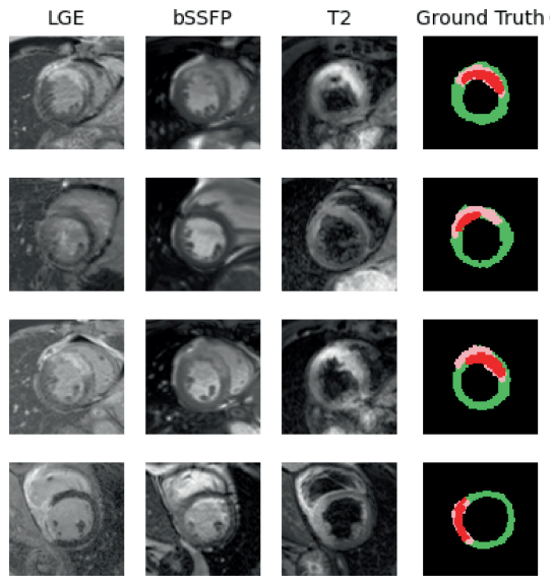
\includegraphics[width=0.86\textwidth]{bab2/ch2-lge-scar.png}
	\caption{Representative LGE-CMR image showing myocardial scar \citep{Margolis2025}}
	\label{fig:ch2-lge-scar}
\end{figure}

Figure~\ref{fig:ch2-lge-scar} illustrates the appearance of myocardial scar in an LGE-CMR image. The hyperenhanced region corresponds to infarcted myocardium, whereas the surrounding darker region represents healthy myocardial tissue. Accurate identification of these regions is essential for reliable myocardial infarction assessment.

\subsection{Clinical Significance of Myocardial Scar Assessment}
\label{subsec:clinical-scar}

Beyond identifying the presence of infarction, myocardial scar assessment provides clinically important information regarding the severity of myocardial damage. Previous studies have demonstrated that larger scar burden is associated with poorer ventricular function, lower recovery potential after revascularization, and an increased risk of adverse cardiac events \citep{Kim2000,Ibanez2018}.

In clinical practice, scar assessment is generally performed by manually outlining infarcted regions on LGE images. Although manual analysis is widely accepted, it is labor-intensive, requires experienced clinicians, and is subject to inter- and intra-observer variability. These limitations become more pronounced when scar boundaries are indistinct or when infarct morphology varies considerably among patients.

\subsection{Automated Myocardial Scar Segmentation}
\label{subsec:auto-scar}

To overcome the limitations of manual analysis, numerous automated and deep learning-based segmentation methods have been proposed. Recent studies have shown that convolutional neural networks, particularly U-Net-based architectures, can accurately identify myocardial scar while substantially reducing analysis time \citep{Oktay2018,Isensee2018}.

The availability of public benchmark datasets has further accelerated research in this area. In particular, the Myocardial Pathology Segmentation (MyoPS) dataset provides standardized multi-sequence CMR images with expert annotations, enabling objective comparison of automated segmentation algorithms under consistent evaluation protocols \citep{Zhuang2019}.

Although considerable progress has been achieved, automated myocardial scar segmentation remains a challenging task. Scar regions often exhibit large variations in size, shape, and image intensity, while the contrast between scar tissue and surrounding myocardium may be weak in some patients. These challenges continue to motivate the development of more reliable deep learning approaches for CMR image analysis.

Besides accurate scar segmentation, effective myocardial infarction assessment also depends on the ability of deep learning models to learn robust image representations. Therefore, the following section reviews the development of artificial intelligence and deep learning techniques for medical image analysis before discussing the segmentation architectures adopted in this dissertation.

\section{Deep Learning in Cardiac Magnetic Resonance Imaging}
\label{sec:dl-cmr}

The growing use of CMR imaging has generated a large amount of imaging data that requires accurate and efficient analysis. Traditionally, cardiac structures and myocardial abnormalities were identified manually by experienced clinicians. Although manual interpretation remains the clinical reference, it is time-consuming, requires substantial expertise, and may produce variations between observers, particularly when image quality is poor or tissue boundaries are difficult to identify \citep{Petitjean2011,Kramer2020}.

To improve efficiency and consistency, researchers initially developed computer-assisted image analysis based on conventional image processing and machine learning techniques. These approaches relied on manually designed features such as image intensity, texture, shape, and edge information before classification or segmentation could be performed. While these methods showed promising results, their performance depended heavily on feature selection and often struggled to handle the large variability found in cardiac MR images \citep{Litjens2017}.

The rapid development of deep learning has significantly changed the way medical images are analyzed. Unlike conventional machine learning, deep learning automatically learns relevant image features directly from training data without requiring manual feature engineering. This capability enables the model to recognize complex anatomical structures and tissue characteristics more effectively, leading to substantial improvements in medical image segmentation performance \citep{LeCun2015,Litjens2017}.

Among various deep learning approaches, Convolutional Neural Networks (CNNs) have become the foundation of most medical image analysis systems. CNNs learn hierarchical image features through convolutional operations, allowing both low-level image patterns and high-level anatomical structures to be represented automatically. As a result, CNN-based methods have demonstrated superior performance in many medical imaging applications, including organ segmentation, lesion detection, disease classification, and image reconstruction \citep{LeCun2015,Shen2017}.

The success of CNNs also accelerated the development of semantic segmentation networks specifically designed for pixel-level image analysis. One important milestone was the introduction of Fully Convolutional Networks (FCNs), which replaced fully connected layers with convolutional layers to generate dense segmentation maps directly from input images. FCNs demonstrated that deep learning could perform end-to-end image segmentation without requiring handcrafted post-processing, opening new opportunities for automated medical image analysis \citep{Long2015}.

Building upon the FCN concept, U-Net was specifically designed for biomedical image segmentation by integrating an encoder--decoder structure with skip connections to preserve fine spatial and anatomical details during feature reconstruction. Owing to its high segmentation accuracy and relatively simple architecture, U-Net has become the most widely adopted backbone for cardiac MR image segmentation and has inspired numerous architectural improvements for different clinical applications \citep{Ronneberger2015,Siddique2021}.

Given its extensive use in cardiac image analysis, understanding the architecture and characteristics of U-Net is essential before discussing more specific components, such as activation functions, pooling strategies, loss functions, residual learning, and attention mechanisms. Therefore, the following section reviews the U-Net architecture as the foundation of many deep learning-based cardiac image segmentation methods.

\section{U-Net Architecture}
\label{sec:unet}

Among various deep learning architectures developed for image segmentation, U-Net has become one of the most widely adopted models in biomedical image analysis. Proposed by \citep{Ronneberger2015}, U-Net was specifically designed to perform accurate pixel-level segmentation using relatively limited training data. Owing to its simple architecture and robust performance, U-Net has been successfully applied to numerous medical imaging applications, including organ segmentation, tumor detection, retinal vessel extraction, brain lesion analysis, and CMR image segmentation \citep{Ronneberger2015,Siddique2021}.

The U-Net architecture consists of two main components, namely an encoder and a decoder, which are connected through skip connections. The encoder progressively extracts increasingly abstract image features while reducing the spatial resolution through convolution and pooling operations. In contrast, the decoder gradually restores the spatial resolution using upsampling operations to generate a pixel-wise segmentation map. Skip connections directly transfer feature information from the encoder to the corresponding decoder layers, allowing fine anatomical details to be preserved during image reconstruction \citep{Ronneberger2015}.

\begin{comment}
Figure~\ref{fig:ch2-unet-architecture} illustrates the overall architecture of U-Net. The encoder learns hierarchical image features from low-level visual patterns to high-level semantic representations, whereas the decoder reconstructs these features into a segmentation map with the same spatial resolution as the input image. The skip connections play an important role in preserving spatial information by combining low-level and high-level features, enabling accurate localization of anatomical structures.

\begin{figure}[htbp]
	\centering
	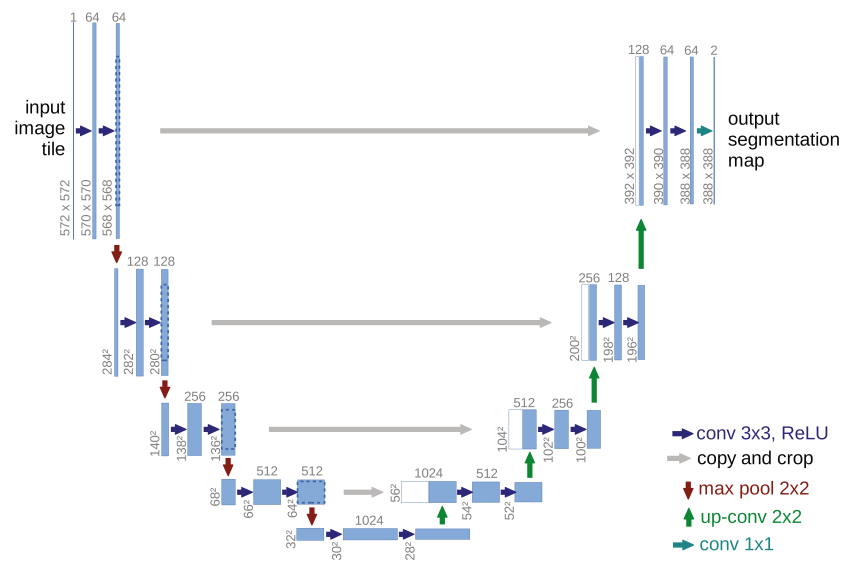
\includegraphics[width=0.75\textwidth]{bab2/ch2-unet-architecture.png}
	\caption{General architecture of U-Net for biomedical image segmentation \citep{Ronneberger2015}}
	\label{fig:ch2-unet-architecture}
\end{figure}
\end{comment}

Because of these advantages, U-Net has become the baseline architecture for many CMR image segmentation studies. It has demonstrated excellent performance in segmenting the left ventricle, right ventricle, and myocardium from cine CMR images, making it one of the most widely adopted architectures in cardiovascular image analysis \citep{Petitjean2011,Bernard2018}.

Despite its success, the segmentation performance of U-Net is still influenced by several components within the network architecture. Previous studies have shown that activation functions affect nonlinear feature learning, pooling mechanisms influence spatial information preservation, and loss functions determine how the network learns from prediction errors during training. In addition, more advanced feature learning strategies have been introduced to further improve segmentation accuracy in challenging medical images. Therefore, these architectural components are reviewed in the following sections as the theoretical foundation for the methods developed in this dissertation.

\section{Activation Functions for Medical Image Segmentation}
\label{sec:activation-functions}

Activation functions are fundamental components of deep neural networks because they introduce nonlinear transformations that enable the network to learn complex feature representations from image data. Without nonlinear activation functions, multiple convolutional layers would behave as a linear transformation, substantially limiting the representational capability of deep neural networks. Consequently, activation functions play an important role in feature extraction, training stability, gradient propagation, and convergence behaviour during network training \citep{Nair2010,Nwankpa2018}.

In medical image segmentation, the influence of activation functions becomes increasingly important because anatomical structures often exhibit low contrast, indistinct boundaries, and considerable morphological variability. These characteristics are particularly evident in CMR images, where accurate segmentation of the left ventricle, right ventricle, and myocardium depends on the network's ability to learn discriminative image features while maintaining stable learning throughout training \citep{Chen2020Review,Hesamian2019}.

Among the numerous activation functions proposed for deep learning, the Rectified Linear Unit (ReLU) has become the most widely adopted because of its computational simplicity and effective mitigation of the vanishing-gradient problem. ReLU preserves positive activation values while suppressing negative responses, thereby facilitating efficient gradient propagation and accelerating network convergence \citep{Nair2010}. The ReLU activation function is defined as

\begin{equation}
	f(x)=\max(0,x)
	\label{eq:relu}
\end{equation}

where $x$ denotes the input activation.

Despite its widespread adoption, ReLU is not without limitations. Since all negative input values are mapped to zero, neurons receiving predominantly negative activations may become permanently inactive during training, a phenomenon commonly referred to as the dying ReLU problem. This limitation may reduce feature diversity and affect segmentation performance, particularly when anatomical boundaries are weak or tissue contrast is limited.

To overcome these limitations, several alternative activation functions have been proposed. One of the most promising is Mish, a smooth self-regularized non-monotonic activation function that preserves a portion of negative activation values while maintaining continuous gradient propagation \citep{Misra2020}. Compared with ReLU, Mish is expected to provide richer feature representation and smoother training behaviour in deep neural networks.

The Mish activation function is expressed as
\begin{equation}
	f(x) = x \tanh\left(\operatorname{softplus}(x)\right),
	\label{eq:mish}
\end{equation}%
where
\begin{equation}
	\operatorname{softplus}(x) = \ln(1+e^x).
	\label{eq:softplus}
\end{equation}

Figure~\ref{fig:ch2-activation-comparison} illustrates the characteristics of the ReLU and Mish activation functions. ReLU generates zero output for all negative inputs while maintaining a linear response for positive values. In contrast, Mish produces a smooth nonlinear response that preserves a portion of negative activations, allowing richer information flow during feature learning. These different characteristics may influence feature representation capability and segmentation performance in deep neural networks.

\begin{figure}[htbp]
	\centering
	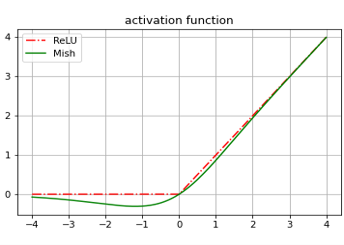
\includegraphics[width=0.62\textwidth]{bab2/ch2-activation-comparison.png}
	\caption{Comparison of the ReLU and Mish activation functions \citep{Riandini2022IST}}
	\label{fig:ch2-activation-comparison}
\end{figure}

Overall, activation functions directly influence how discriminative image features are learned throughout the training process. Since CMR segmentation requires accurate delineation of complex cardiac structures with subtle anatomical boundaries, selecting an appropriate activation function represents an important consideration in improving segmentation performance. Besides activation functions, another fundamental component that strongly influences feature representation is the pooling mechanism used during feature downsampling. Therefore, the following section reviews pooling mechanisms commonly employed in deep learning-based medical image segmentation.

\section{Pooling Mechanisms for Medical Image Segmentation}
\label{sec:pooling}

Pooling is an essential operation in convolutional neural networks because it reduces the spatial dimensions of feature maps while preserving representative image information. By progressively reducing the feature map size, pooling decreases computational complexity, enlarges the receptive field, and improves computational efficiency. Consequently, pooling has become a fundamental component of deep learning models for medical image segmentation \citep{Goodfellow2016,Chen2020Review}.

Among the available pooling strategies, Max Pooling is the most widely adopted because of its simple implementation and computational efficiency. During the pooling process, only the largest activation value within a local neighborhood is retained, while the remaining activation values are discarded. This operation effectively preserves the most dominant feature response and is mathematically defined as

\begin{equation}
	P_{\max}=\max(x_1,x_2,\ldots,x_n)
	\label{eq:max-pooling}
\end{equation}

where $x_i$ represents the activation values within a pooling window.

Although Max Pooling has demonstrated satisfactory performance in many segmentation tasks, retaining only the maximum activation may discard useful local information. This limitation becomes particularly important in CMR image segmentation because the myocardium appears as a relatively thin structure with subtle anatomical boundaries. As a result, repeated downsampling may gradually reduce boundary information and affect segmentation accuracy.

To overcome this limitation, several alternative pooling strategies have been proposed. One of these is Fuzzy Logic-Based Pooling, which incorporates fuzzy set theory into the pooling process by assigning a membership value to each activation before computing the pooled feature. Instead of selecting only the strongest activation, fuzzy pooling allows information from all activation values to contribute to the pooled representation according to their corresponding membership coefficients. This strategy preserves richer local contextual information while reducing information loss during feature downsampling \citep{Zadeh1965,Diamantis2020}.

The generalized fuzzy pooling operation is expressed as

\begin{equation}
	P_{\mathrm{fuzzy}}=\frac{\sum_{i=1}^{n}\mu_i x_i}{\sum_{i=1}^{n}\mu_i}
	\label{eq:fuzzy-pooling}
\end{equation}

where $x_i$ denotes the activation value, $\mu_i$ represents the corresponding fuzzy membership coefficient, and $n$ denotes the number of activation values within the pooling window.

\begin{comment}
\begin{figure}[htbp]
	\centering
	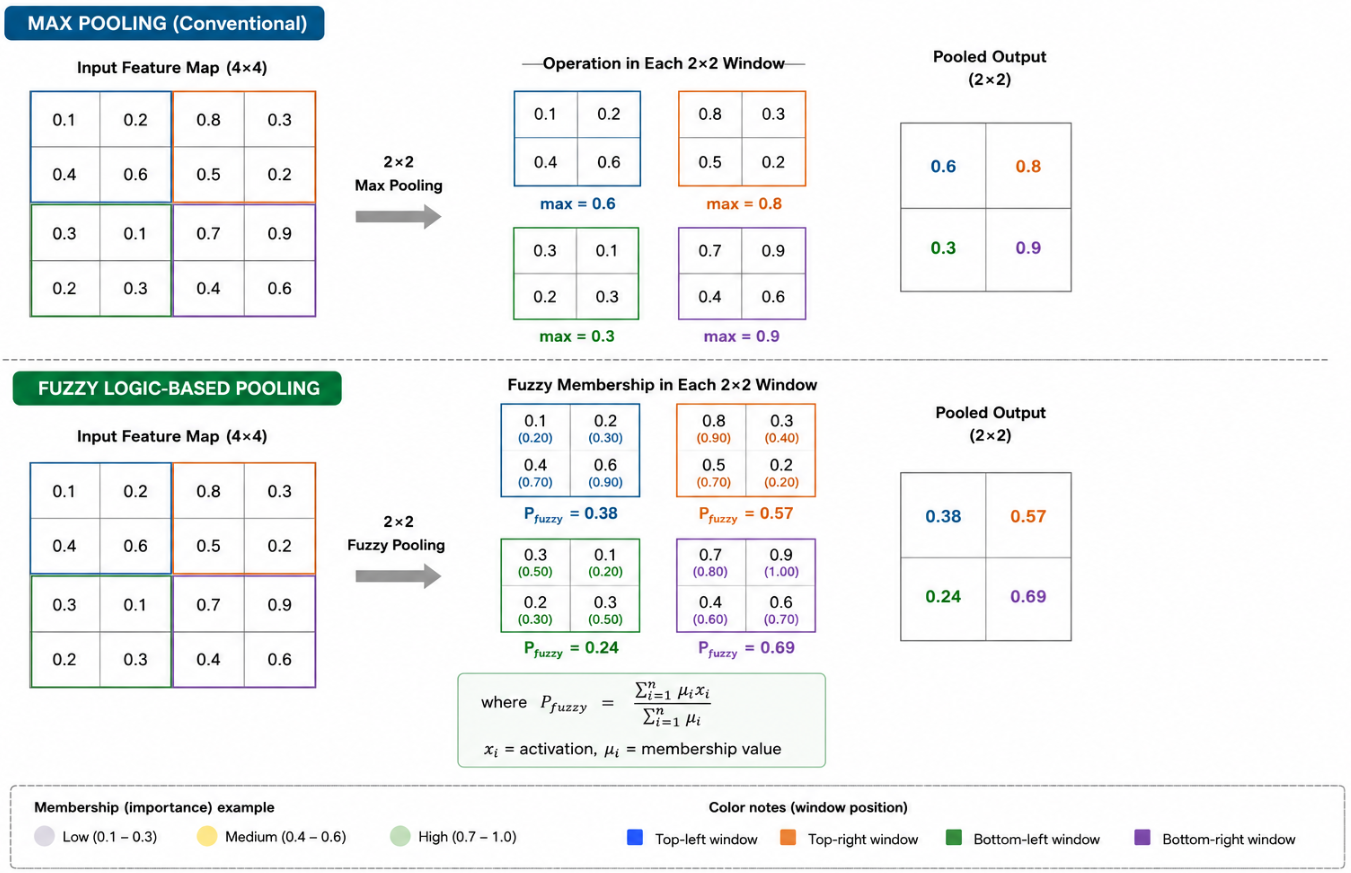
\includegraphics[width=0.86\textwidth]{bab2/ch2-pooling-comparison.png}
	\caption{Example of comparison between conventional max pooling and fuzzy logic-based pooling}
	\label{fig:ch2-pooling-comparison}
\end{figure}

Figure~\ref{fig:ch2-pooling-comparison} illustrates the conceptual difference between the two pooling strategies. Max Pooling preserves only the strongest activation within each pooling window, whereas Fuzzy Logic-Based Pooling aggregates information from all activation values according to their membership coefficients. Consequently, fuzzy pooling is able to preserve richer spatial information and better maintain anatomical continuity during feature extraction.
\end{comment}

Overall, the pooling mechanism has a direct influence on feature representation learned by deep neural networks. Since accurate CMR segmentation depends on preserving thin myocardial boundaries and subtle anatomical structures, selecting an appropriate pooling strategy remains an important consideration for improving segmentation performance. Besides feature extraction, segmentation performance is also influenced by the learning objective used during network training. Therefore, the following section reviews the loss functions commonly employed in deep learning-based medical image segmentation.

\section{Loss Functions for Medical Image Segmentation}
\label{sec:loss-functions}

Loss functions play a fundamental role in deep learning because they measure the discrepancy between the predicted output and the corresponding ground-truth annotation during network training. The computed loss is subsequently minimized through backpropagation, enabling the network to progressively improve its segmentation performance. Consequently, the choice of an appropriate loss function directly influences learning behaviour, convergence stability, and the final segmentation accuracy \citep{Jadon2020,Ma2021}.

In medical image segmentation, selecting an appropriate loss function is particularly important because the target anatomy often occupies only a small portion of the image. Under such conditions, conventional loss functions may become dominated by background pixels, making it difficult for the network to accurately learn small anatomical structures and object boundaries. To address this challenge, various loss functions have been developed, each emphasizing different learning objectives.

One of the most widely used objective functions is Cross-Entropy Loss, which evaluates the difference between the predicted class probabilities and the corresponding ground-truth labels. Because of its simple formulation and stable training behaviour, Cross-Entropy Loss has become the standard objective function for many image classification and segmentation tasks.

The Cross-Entropy Loss is defined as

\begin{equation}
	\mathcal{L}_{\mathrm{CE}}=-\sum_{i=1}^{C} y_i\log(\hat{y}_i)
	\label{eq:cross-entropy}
\end{equation}

where $y_i$ denotes the ground-truth label, $\hat{y}_i$ represents the predicted probability, and $C$ is the total number of classes.

Although Cross-Entropy Loss performs well for balanced datasets, its effectiveness may decrease when the target object occupies only a limited image area. Consequently, several overlap-based loss functions have been introduced for medical image segmentation.

Among these, Dice Loss has become one of the most commonly adopted because it directly maximizes the overlap between the predicted segmentation and the reference annotation. Since Dice Loss focuses on region similarity rather than individual pixel classification, it is generally more robust to class imbalance than Cross-Entropy Loss \citep{Milletari2016}.

Another widely adopted objective function is Focal Loss, which extends Cross-Entropy Loss by assigning greater weight to difficult training samples while reducing the contribution of easily classified pixels. This enables the network to focus more effectively on small or challenging regions that are frequently misclassified \citep{Lin2017}.

To further improve segmentation overlap, Lov\'asz-Softmax Loss was proposed as a differentiable surrogate for the Intersection over Union (IoU) metric. Unlike conventional pixel-wise loss functions, Lov\'asz-Softmax directly improves segmentation overlap, making it particularly suitable for semantic segmentation tasks in which IoU is used as the primary evaluation metric \citep{Berman2018}.

\begin{table}[htbp]
	\centering
	\caption{Comparison of representative loss functions for medical image segmentation} %\cite{Berman2018,Jadon2020,Lin2017,Milletari2016}}
	\label{tab:loss-functions}
	
	\small
	\renewcommand{\arraystretch}{1.2}
	\begin{tabular}{
			>{\raggedright\arraybackslash}p{0.18\textwidth}
			>{\raggedright\arraybackslash}p{0.27\textwidth}
			>{\raggedright\arraybackslash}p{0.27\textwidth}
			>{\raggedright\arraybackslash}p{0.20\textwidth}
		}
		\toprule
		\textbf{Loss Function} & \textbf{Main Characteristic} & \textbf{Strength} & \textbf{Limitation} \\ \midrule
		Cross-Entropy & Pixel-wise classification & Stable training and simple implementation & Sensitive to class imbalance \\
		Dice Loss & Region overlap & Effective for imbalanced segmentation tasks & May be less stable during early training \\
		Focal Loss & Weighted learning of difficult samples & Improves learning of small target regions & Requires additional parameter tuning \\
		Lov\'asz-Softmax & Direct optimization of IoU & Improves region overlap & Higher computational complexity \\ \bottomrule
	\end{tabular}
	
	\vspace{4pt}
	{\raggedright \footnotesize \textit{Source:} Adapted from \cite{Milletari2016}, \cite{Lin2017}, \cite{Berman2018}, and \cite{Jadon2020}.\par}
\end{table}

Table~\ref{tab:loss-functions} summarizes the characteristics of the most widely used loss functions for medical image segmentation. Each loss function emphasizes a different learning objective and therefore exhibits different training behaviour. Consequently, selecting an appropriate loss function should consider the characteristics of the segmentation task, including class imbalance, object size, boundary complexity, and the evaluation metric used.

Overall, previous studies demonstrate that no single loss function consistently achieves the best performance across all segmentation tasks. Instead, the effectiveness of a loss function depends on the characteristics of the image data and the anatomical structures being segmented. Therefore, investigating suitable loss functions remains an important aspect of improving CMR image segmentation. Besides the learning objective, segmentation performance can also be enhanced through more effective feature extraction and feature refinement. These aspects are discussed in the following section on residual learning and attention mechanisms.

\section{Residual Learning and Attention Mechanisms}
\label{sec:residual-attention}

Residual learning and attention mechanisms have become important architectural components in modern deep learning models for medical image segmentation. Although U-Net has demonstrated excellent performance in various segmentation tasks, accurately identifying small anatomical structures and preserving fine boundaries remain challenging, particularly in CMR images. Consequently, many recent studies have incorporated residual learning and attention mechanisms to improve feature representation and segmentation accuracy \citep{He2016,Oktay2018,Schlemper2019}.

Residual learning was introduced to address the degradation problem encountered when neural networks become deeper. Instead of learning the complete feature transformation, shortcut connections allow feature information from earlier layers to be directly propagated to deeper layers. This mechanism facilitates gradient propagation, improves learning stability, and enables the network to learn more discriminative image features without substantially increasing training difficulty \citep{He2016}.

Attention mechanisms complement residual learning by enabling the network to focus on the most informative image regions while suppressing irrelevant background information. Rather than treating every feature equally, attention mechanisms assign different levels of importance to feature maps according to their relevance to the segmentation task. This selective feature learning improves the network's ability to identify anatomical structures and pathological regions with greater accuracy \citep{Oktay2018,Woo2018}.

The combination of residual learning and attention mechanisms has been successfully applied to various medical image segmentation tasks because they address different aspects of feature learning. Residual learning improves information propagation and learning stability, whereas attention mechanisms enhance the network's ability to emphasize diagnostically important regions. These complementary characteristics have made both approaches widely adopted in recent deep learning-based medical image segmentation studies, including CMR image analysis.

\section{Evaluation Metrics}
\label{sec:evaluation-metrics}

Objective performance evaluation is essential for assessing the reliability of deep learning models in medical image segmentation. Since no single metric can comprehensively represent segmentation quality, multiple complementary evaluation metrics are commonly employed to assess region overlap, boundary accuracy, and quantitative agreement. Accordingly, this dissertation evaluates the proposed framework using the Dice Similarity Coefficient (DSC), Intersection over Union (IoU), Hausdorff Distance (HD), Mean Absolute Error (MAE), Pearson Correlation Coefficient (PCC), and Bland--Altman analysis, which are widely adopted in medical image analysis \citep{Taha2015,Zou2004}.

Among these metrics, the Dice Similarity Coefficient (DSC) and Intersection over Union (IoU) are the most frequently used to evaluate segmentation accuracy because they quantify the degree of overlap between the predicted segmentation and the corresponding ground-truth annotation. A higher value indicates better agreement between the two segmentation results \citep{Milletari2016,Taha2015}.

The Dice Similarity Coefficient is defined as

\begin{equation}
	\mathrm{DSC}=\frac{2|P\cap G|}{|P|+|G|}
	\label{eq:dsc}
\end{equation}

where $P$ and $G$ denote the predicted segmentation and the corresponding ground-truth annotation.

Similarly, the Intersection over Union is calculated as

\begin{equation}
	\mathrm{IoU}=\frac{|P\cap G|}{|P\cup G|}
	\label{eq:iou}
\end{equation}

where a larger IoU value indicates greater segmentation consistency.

Besides evaluating region overlap, accurate boundary localization is also important in CMR image segmentation. Therefore, the Hausdorff Distance (HD) is used to measure the maximum distance between the predicted and reference boundaries, providing complementary information regarding boundary accuracy that cannot be captured by overlap-based metrics alone \citep{Taha2015}.

Structural Similarity Index (SSIM) evaluates the similarity between the predicted and reference images by considering luminance, contrast, and structural information. An SSIM value closer to 1 indicates greater structural similarity. In this dissertation, SSIM is used as an additional indicator of structural consistency in the generated segmentation results.

For quantitative myocardial scar assessment, the agreement between the estimated and reference scar measurements is evaluated using the Mean Absolute Error (MAE), Pearson Correlation Coefficient (PCC), and Bland--Altman analysis. MAE measures the average estimation error, PCC evaluates the strength of the linear relationship between two measurements, whereas Bland--Altman analysis assesses their level of agreement by examining the measurement bias and the corresponding limits of agreement. These complementary metrics are widely used to determine the reliability and clinical applicability of quantitative measurement methods \citep{Bland1986,Giavarina2015}.

\begin{table}[htbp]
	\centering
	\caption{Commonly used evaluation metrics for medical image segmentation and quantitative scar assessment}
	\label{tab:evaluation-metrics}
	\begin{tabularx}{\textwidth}{
			>{\raggedright\arraybackslash}p{0.35\textwidth}
			>{\raggedright\arraybackslash}X
			>{\raggedright\arraybackslash}p{0.18\textwidth}
		}
		\toprule
		\textbf{Metric} & \textbf{Purpose} & \textbf{Ideal Value} \\
		\midrule
		Dice Similarity Coefficient (DSC) & Measures region overlap & 1.0 \\
		Intersection over Union (IoU) & Measures segmentation overlap & 1.0 \\
		Hausdorff Distance (HD) & Measures boundary discrepancy & 0 \\
		Structural Similarity Index (SSIM) & Measures structural similarity & 1.0 \\
		Mean Absolute Error (MAE) & Measures quantitative estimation error & 0 \\
		Pearson Correlation Coefficient (PCC) & Measures linear correlation & 1.0 \\
		Bland--Altman analysis & Assesses agreement between measurements & Small bias and narrow limits of agreement \\
		\bottomrule
	\end{tabularx}
	
	\vspace{4pt}
	{\raggedright \footnotesize \textit{Source:} Adapted from \cite{Bland1986}, \cite{Taha2015}, and \cite{Giavarina2015}.\par}
\end{table}

Table~\ref{tab:evaluation-metrics} summarizes the evaluation metrics utilized in this dissertation. While DSC, IoU, and HD evaluate segmentation quality from different perspectives, MAE, PCC, and Bland--Altman analysis assess the reliability of quantitative myocardial scar measurements. Together, these metrics provide a comprehensive evaluation framework for the deep learning models developed in Chapters IV, V, and VI.

\section{Related Works and Research Gap}
\label{sec:related-work}

Deep learning has significantly advanced the analysis of CMR images, particularly for cardiac structure segmentation and myocardial scar assessment. Numerous studies have demonstrated that convolutional neural networks, especially U-Net and its variants, are capable of producing accurate segmentation of the left ventricle, right ventricle, myocardium, and myocardial scar regions. These developments have substantially improved the efficiency and reproducibility of cardiac image analysis compared with conventional manual delineation methods \citep{Ronneberger2015,Bernard2018,Chen2020Review}.

Recent studies have also investigated various strategies to improve segmentation performance. These include the selection of appropriate activation functions, the development of alternative pooling mechanisms, the investigation of different loss functions to address class imbalance, and the incorporation of residual learning and attention mechanisms to enhance feature representation. Although these approaches have individually demonstrated promising results, most previous studies focused on improving only a single component of the segmentation framework, while relatively few have investigated how these complementary components can be systematically integrated into a unified workflow for myocardial infarction assessment.

\begin{landscape}
	\begin{table}[htbp]
		\centering
		\caption{Summary of representative studies on deep learning-based CMR image analysis}
		\label{tab:related-studies}
		
		\small
		\renewcommand{\arraystretch}{1.3}
		\begin{tabular}{
				>{\raggedright\arraybackslash}p{0.20\linewidth}
				>{\raggedright\arraybackslash}p{0.22\linewidth}
				>{\raggedright\arraybackslash}p{0.28\linewidth}
				>{\raggedright\arraybackslash}p{0.26\linewidth}
			}
			\toprule
			\textbf{Reference} & \textbf{Research Focus} & \textbf{Main Contribution} & \textbf{Main Limitation} \\ \midrule
			
			\cite{Ronneberger2015} & 
			U-Net & 
			Encoder--decoder architecture for biomedical image segmentation & 
			Uses standard network components without investigating architectural variants \\ \addlinespace
			
			\cite{Bernard2018} & 
			Cardiac MRI segmentation & 
			Benchmark evaluation for cardiac structure segmentation & 
			Focused primarily on cardiac structure segmentation \\ \addlinespace
			
			\cite{Oktay2018} & 
			Attention U-Net & 
			Attention mechanism for improved feature localization & 
			Did not address myocardial scar quantification \\ \addlinespace
			
			\cite{Ma2021} & 
			Residual learning & 
			Improved feature propagation using shortcut connections & 
			Developed for general computer vision applications \\ \addlinespace
			
			\cite{Lin2017} & 
			Focal Loss & 
			Improved learning from class-imbalanced data & 
			Focused for object detection rather than medical image segmentation \\ \addlinespace
			
			\cite{Berman2018} & 
			Lov\'asz-Softmax Loss & 
			Direct optimization of the IoU metric & 
			Focused on general semantic segmentation problems \\ \addlinespace
			
			Recent CMR studies & 
			Myocardial scar segmentation & 
			Improved automatic scar segmentation & 
			Most studies improve individual components independently \\
			\bottomrule
		\end{tabular}
	\end{table}
\end{landscape}

Table~\ref{tab:related-studies} shows that previous studies have achieved considerable progress in individual aspects of CMR image analysis. Nevertheless, most investigations focus on a single methodological component, such as network architecture, feature extraction, pooling strategy, loss function, or attention mechanism. As a result, the potential benefits of combining these complementary approaches within a unified analysis framework have not been fully explored.

Based on the reviewed literature, several research gaps can be identified. First, many studies emphasize improvements in cardiac structure segmentation but provide limited investigation into how segmentation quality influences subsequent myocardial scar analysis. Second, although various loss functions have been proposed to address class imbalance, comprehensive comparative investigations under identical experimental conditions remain limited. Third, residual learning and attention mechanisms have demonstrated promising performance for medical image segmentation, yet their application to quantitative myocardial scar assessment has received relatively limited attention. Finally, relatively few studies have presented an integrated deep learning framework that combines accurate cardiac structure segmentation, reliable myocardium segmentation, and myocardial scar quantification within a single workflow for myocardial infarction assessment.

These research gaps form the scientific basis of this dissertation. Accordingly, the research presented in the following chapters is organized into three complementary stages. Chapter IV investigates cardiac structure segmentation using an enhanced U-Net with an improved pooling strategy. Chapter V evaluates different loss functions to achieve more reliable myocardium segmentation. Finally, Chapter VI develops a residual attention-based framework for myocardial scar segmentation and quantitative scar assessment. Collectively, these studies establish an integrated deep learning framework for CMR image analysis to support myocardial infarction assessment.

		%\cleardoublepage
		\clearpage
		
		\chapter{RESEARCH METHODOLOGY}
\label{chap:3}

\section{Research Framework}
\label{sec:research-framework}

This research proposes a deep learning-based framework for automated analysis of CMR images to support myocardial infarction assessment. The network integrates cardiac structure segmentation, myocardial scar assessment, and quantitative scar area measurement into a unified workflow. Instead of treating these tasks as independent processes, the output generated at each stage serves as the input for the subsequent stage, establishing a systematic framework for myocardial infarction assessment. The overall research method is presented in Figure~\ref{fig:ch3-research-stages} \citep{Ronneberger2015,Bernard2018,Zhuang2020}.

The proposed framework utilizes two publicly available CMR datasets with different roles. The Automated Cardiac Diagnosis Challenge (ACDC) dataset is used for cardiac structure segmentation because it provides expert annotations of the left ventricle, right ventricle, and myocardium at both End-Diastole (ED) and End-Systole (ES). Subsequently, the Myocardial Pathology Segmentation (MyoPS2020) dataset is used for myocardial scar assessment based on complementary multi-sequence CMR images, including balanced steady-state free precession (bSSFP), T2-weighted imaging (T2WI), and Late Gadolinium Enhancement (LGE). The use of these two datasets enables each stage of the proposed framework to be developed using data that are specifically designed for its corresponding objective \citep{Bernard2018,Zhuang2020}.

The framework begins with cardiac structure segmentation using a U-Net-based architecture to identify the left ventricle, right ventricle, and myocardium from cine CMR images. To establish a reliable segmentation framework, the proposed method investigates the activation function, pooling strategy, and loss function while maintaining a consistent network architecture throughout the experiments. The resulting myocardium segmentation subsequently defines the anatomical region used for myocardial scar assessment, thereby establishing the anatomical foundation for the subsequent scar analysis \citep{Ronneberger2015,Diamantis2020,Riandini2025Array}.

Following cardiac structure segmentation, myocardial scar assessment is performed using the MyoPS2020 dataset. Rather than transferring segmentation masks between datasets, the anatomical knowledge established through the cardiac structure segmentation framework is independently applied to define the myocardium region for myocardial scar assessment within the MyoPS2020 dataset, thereby providing the anatomical region used for subsequent myocardial scar analysis.

Finally, the proposed framework is evaluated using quantitative performance metrics appropriate for both segmentation and scar area quantification. The methodology presented in this chapter provides the foundation for the implementation and experimental investigations described in Chapters IV, V, and VI.

\begin{figure}[htbp]
	\centering
	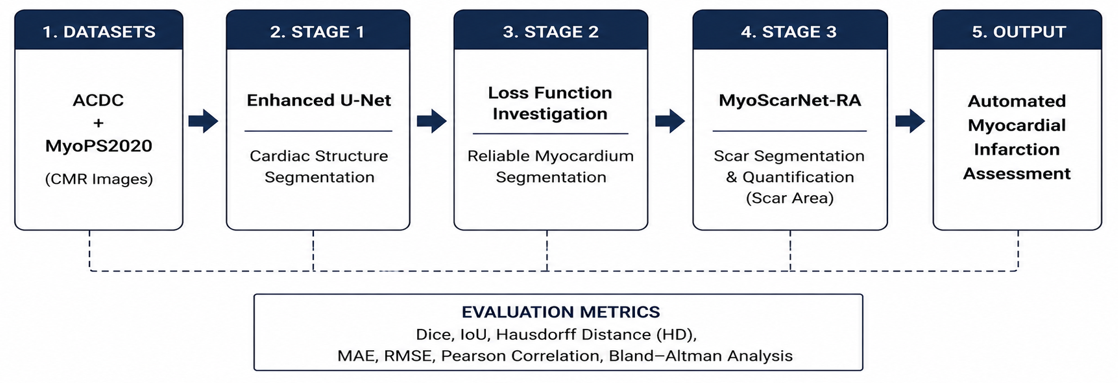
\includegraphics[width=0.86\textwidth]{bab3/ch3-research-stages.png}
	\caption{Overall Research Framework of the Proposed Deep Learning-Based CMR Image Analysis for Myocardial Infarction Assessment}
	\label{fig:ch3-research-stages}
\end{figure}

\section{Research Dataset and Dataset Preparation}
\label{sec:dataset-preparation}

This research utilizes two publicly available CMR datasets, namely the Automated Cardiac Diagnosis Challenge (ACDC) dataset and the Myocardial Pathology Segmentation (MyoPS2020) dataset. Before model development, each dataset was prepared according to the requirements of its respective study. The ACDC dataset was prepared for cardiac structure segmentation in Chapters IV and V, whereas the MyoPS2020 dataset underwent an independent preparation procedure for myocardial scar segmentation and quantitative scar assessment in Chapter VI.

\subsection{Automated Cardiac Diagnosis Challenge (ACDC) Dataset}
\label{subsec:acdc-dataset}

The Automated Cardiac Diagnosis Challenge (ACDC) dataset was used for cardiac structure segmentation. The dataset consists of cine CMR images with expert annotations of the left ventricle (LV), right ventricle (RV), and myocardium (MYO) acquired at both End-Diastole (ED) and End-Systole (ES). These reference annotations provide the ground truth required for training and evaluating the proposed segmentation framework \citep{Bernard2018}.

Representative examples of the cine CMR images and their corresponding manual annotations at End-Diastole (ED) and End-Systole (ES) phases are presented in %
% Figure~\ref{fig:ch3-acdc-examples_a} and Figure~\ref{fig:ch3-acdc-examples_b} (or 
Figure~\ref{fig:ch3-acdc-examples}, while the principal characteristics of the dataset are summarized in Table~\ref{tab:acdc-characteristics}.

\begin{figure}[htbp]
	\centering
	\begin{minipage}{0.85\textwidth}
		\centering
		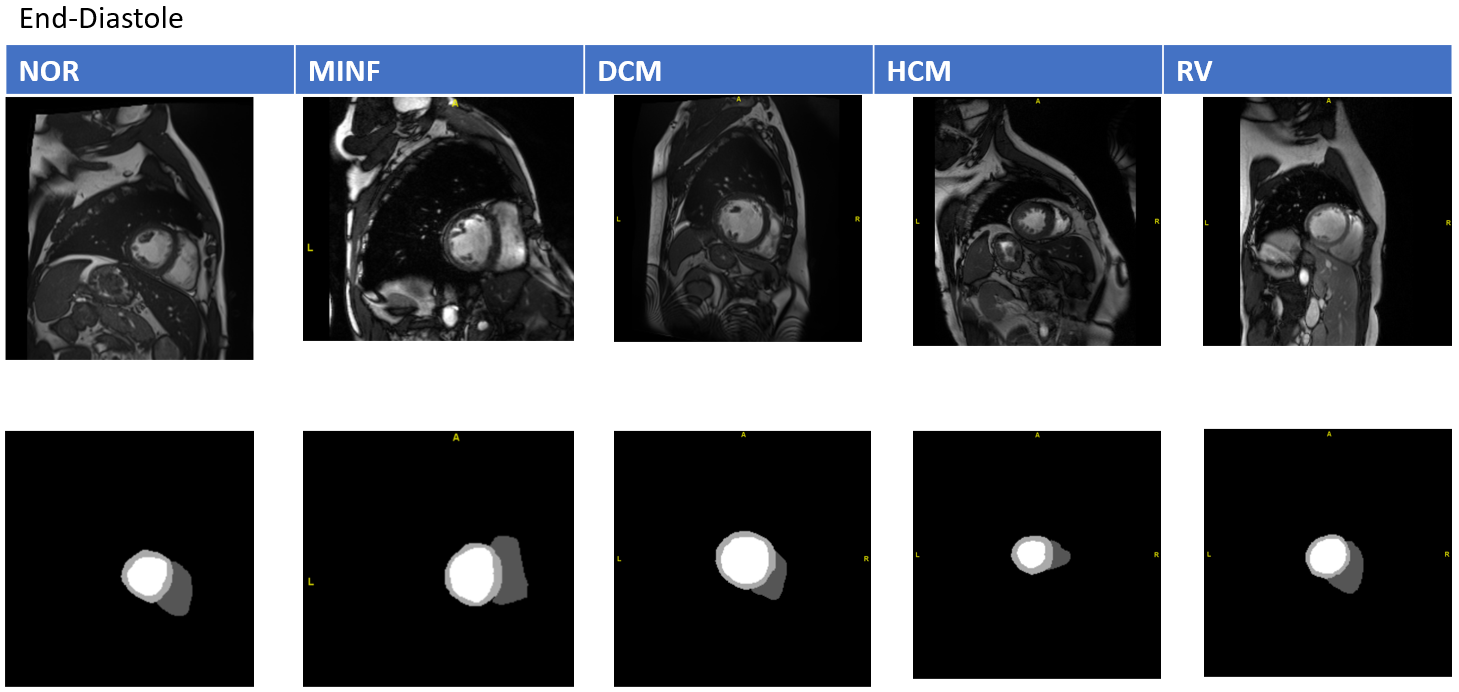
\includegraphics[width=\textwidth]{bab3/ch3-acdc-examples_a.png}
		\centerline{\small (a) End-Diastole (ED) phase}
		\label{fig:ch3-acdc-examples_a}
	\end{minipage}
	
	\vspace{1.5ex}
	
	\begin{minipage}{0.85\textwidth}
		\centering
		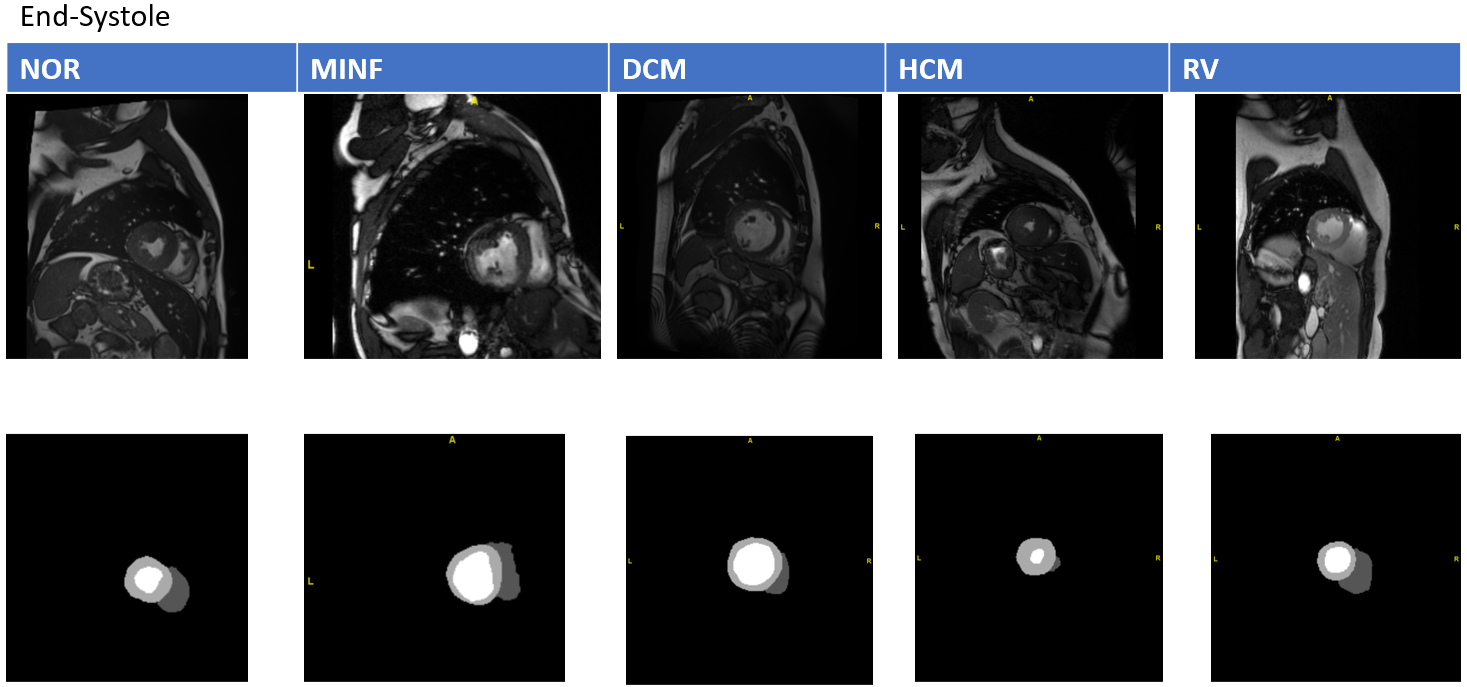
\includegraphics[width=\textwidth]{bab3/ch3-acdc-examples_b.png}
		\centerline{\small (b) End-Systole (ES) phase}
		\label{fig:ch3-acdc-examples_b}
	\end{minipage}
	
	\caption{Representative cine CMR images and corresponding manual annotations from the ACDC dataset \citep{Bernard2018}: (a) End-Diastole (ED) phase, and (b) End-Systole (ES) phase.}
	\label{fig:ch3-acdc-examples}
\end{figure}

\begin{table}[htbp]
\centering
\caption{Characteristics of the ACDC dataset}
\label{tab:acdc-characteristics}
\begin{tabularx}{\textwidth}{p{0.30\textwidth} X}
\toprule
\textbf{Characteristic} & \textbf{Description} \\
\midrule
Dataset & Automated Cardiac Diagnosis Challenge (ACDC) \\
Imaging modality & Cine CMR \\
Number of subjects & 150 \\
Cardiac phases & End-Diastole (ED) and End-Systole (ES) \\
Reference annotations & Left ventricle (LV), right ventricle (RV), and myocardium (MYO) \\
Purpose in this study & Cardiac structure segmentation (Chapters IV and V) \\
\bottomrule
\end{tabularx}

\vspace{4pt}
{\raggedright \footnotesize \textit{Source:} Adapted from \citet{Bernard2018}.\par}
\end{table}

\subsection{Myocardial Pathology Segmentation (MyoPS2020) Dataset}
\label{subsec:myops-dataset}

The Myocardial Pathology Segmentation (MyoPS2020) dataset was used for myocardial scar assessment. Unlike the ACDC dataset, which focuses on cardiac structure segmentation, MyoPS2020 provides complementary multi-sequence CMR images consisting of balanced steady-state free precession (bSSFP), T2-weighted imaging (T2WI), and Late Gadolinium Enhancement (LGE), together with expert annotations of myocardial pathology. These complementary image sequences enable myocardial scar assessment using anatomical and pathological information acquired from different CMR modalities \citep{Zhuang2020}.

Representative examples of the multi-sequence CMR images are presented in Figure~\ref{fig:ch3-myops-examples}, whereas the principal characteristics of the dataset are summarized in Table~\ref{tab:myops-characteristics}.

\begin{figure}[htbp]
	\centering
	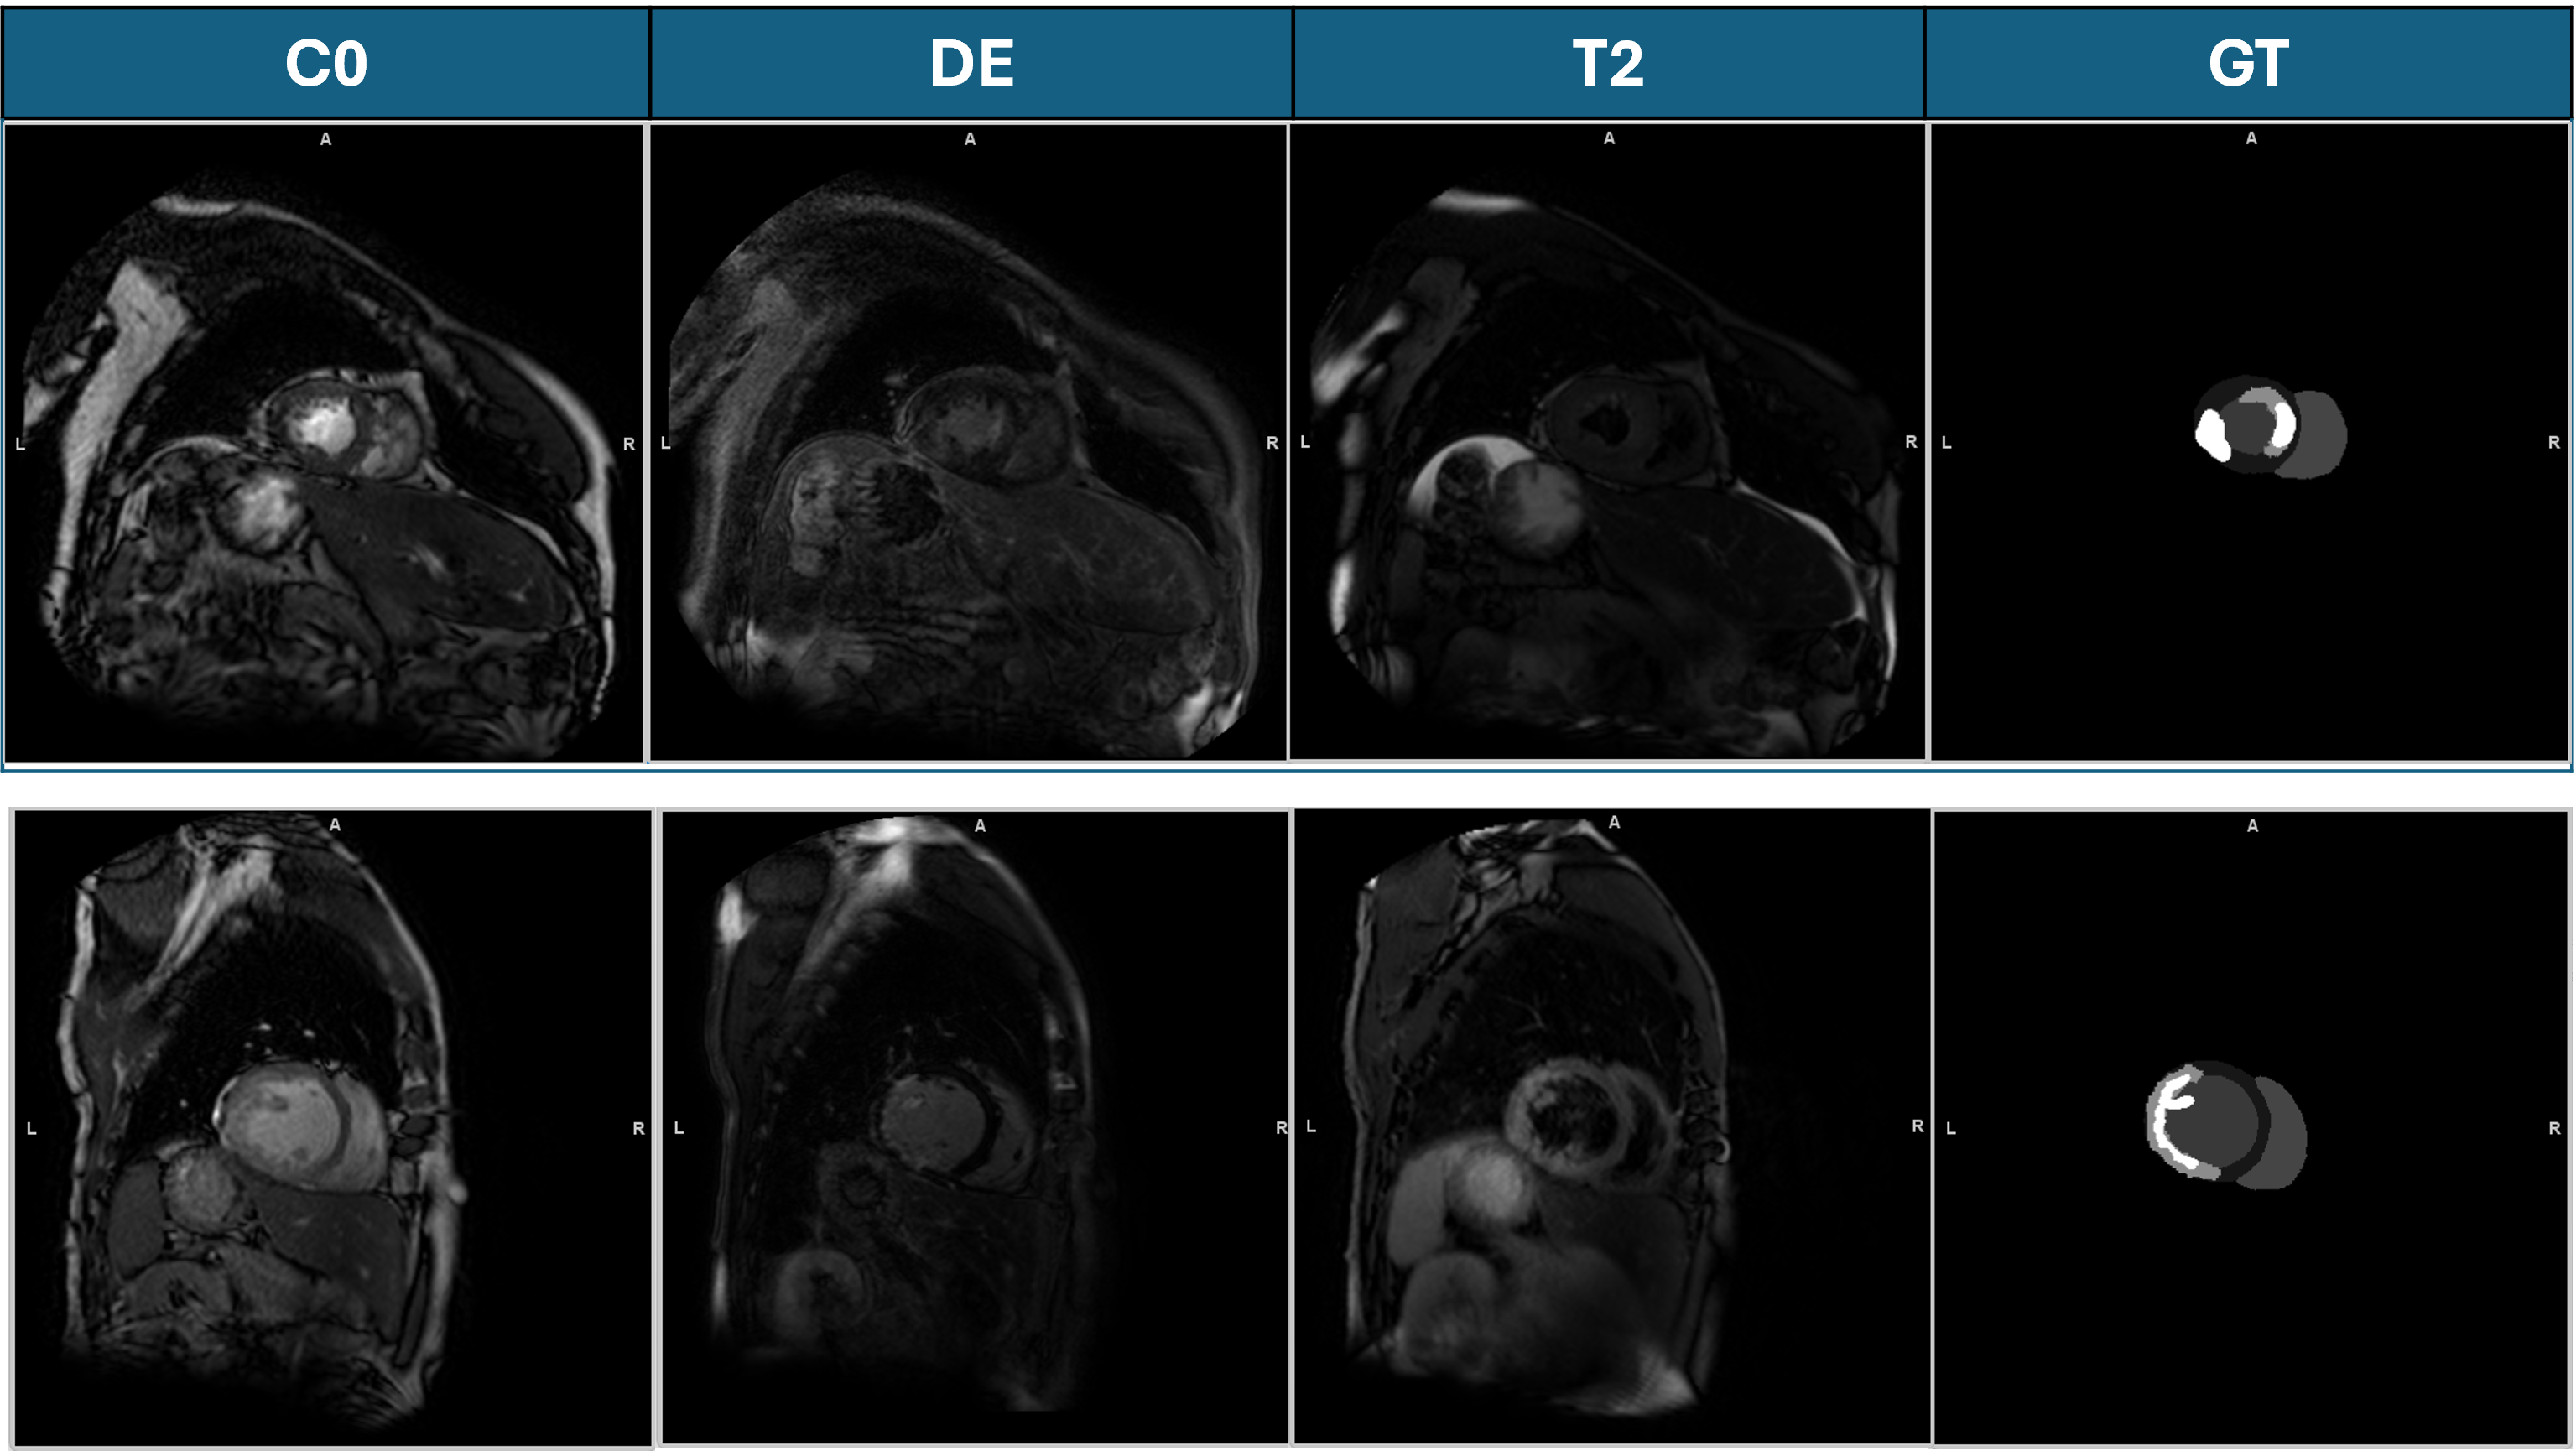
\includegraphics[width=0.86\textwidth]{bab3/ch3-myops-examples.png}
	\caption{Representative multi-sequence CMR images from the MyoPS2020 dataset \citep{Zhuang2020}}
	\label{fig:ch3-myops-examples}
\end{figure}

\begin{table}[htbp]
	\centering
	\caption{Characteristics of the MyOPS2020 dataset}
	\label{tab:myops-characteristics}
	
	% Mengubah tipe kolom X agar rata kiri tanpa membuat spasi melebar
	\begin{tabularx}{\textwidth}{p{0.30\textwidth} >{\raggedright\arraybackslash}X}
		\toprule
		\textbf{Characteristic} & \textbf{Description} \\ \midrule
		Dataset & Myocardial Pathology Segmentation (MyoPS2020) \\
		Imaging modality & Multi-sequence CMR \\
		Number of subjects & 45 \\
		Image sequences & bSSFP, T2WI, and LGE \\
		Reference annotations & Myocardium, edema, and myocardial scar \\
		Purpose in this study & Myocardial scar assessment (Chapter VI) \\ \bottomrule
	\end{tabularx}
\vspace{4pt}
{\raggedright \footnotesize \textit{Source:} Adapted from \citet{Zhuang2020}.\par}
\end{table}

\subsection{Dataset Preparation}
\label{subsec:dataset-preparation}

Before model development, images from the ACDC and MyoPS2020 datasets were prepared using a consistent procedure to ensure compatibility throughout the experiments. Although both datasets underwent image resizing and intensity normalization, the preparation procedure was performed independently according to the objective of each study. The ACDC dataset was prepared for cardiac structure segmentation, whereas the MyoPS2020 dataset was independently prepared for myocardial scar assessment.

Image resizing was first performed to produce a uniform input size for all experiments. Subsequently, intensity normalization was applied to reduce image intensity variations among CMR images acquired from different subjects and imaging conditions. Finally, each dataset was partitioned into training, validation, and testing subsets according to the experimental protocol adopted in this study. The overall dataset preparation procedure is illustrated in Figure~\ref{fig:ch3-dataset-preparation}.

\begin{figure}[htbp]
	\centering
	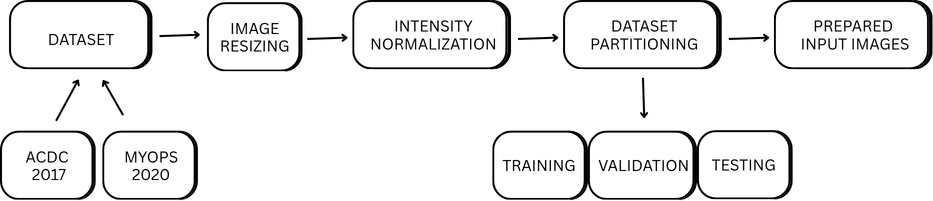
\includegraphics[width=0.86\textwidth]{bab3/ch3-dataset-preparation.png}
	\caption{Overview of the dataset preparation procedure}
	\label{fig:ch3-dataset-preparation}
\end{figure}

As illustrated in Figure~\ref{fig:ch3-dataset-preparation}, both datasets underwent the same general preprocessing stages, including image resizing, intensity normalization, and dataset partitioning. However, each dataset was prepared independently according to its respective research objective, thereby providing standardized inputs for cardiac structure segmentation and myocardial scar assessment.

\section{Cardiac Structure Segmentation}
\label{sec:cardiac-structure-segmentation}

Cardiac structure segmentation represents the first stage of the proposed framework. The objective of this stage is to automatically identify the left ventricle (LV), right ventricle (RV), and myocardium (MYO) from cine CMR images. The resulting myocardium segmentation provides the anatomical information required for the subsequent myocardial scar assessment. Consequently, reliable cardiac structure segmentation establishes the foundation for the overall myocardial infarction assessment framework proposed in this dissertation.

To accomplish this objective, a U-Net-based architecture was adopted as the baseline segmentation framework. Rather than introducing a new network architecture, this study systematically investigates several methodological components that may influence segmentation performance while maintaining the same baseline architecture throughout the experiments. These investigations include activation function selection, fuzzy pooling integration, and loss function investigation. The overall workflow of the cardiac structure segmentation stage is illustrated in Figure~\ref{fig:ch3-cardiac-framework}.

\begin{figure}[htbp]
	\centering
	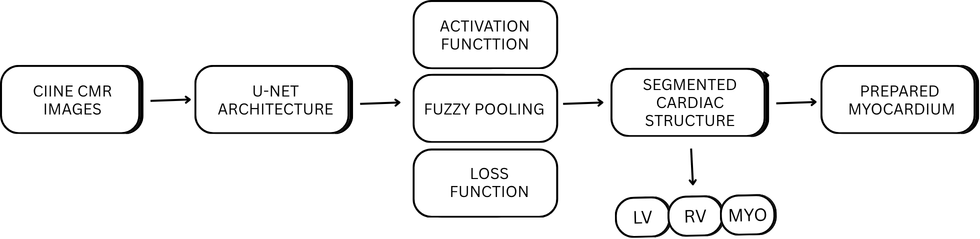
\includegraphics[width=0.86\textwidth]{bab3/ch3-cardiac-framework.png}
	\caption{Overview of the cardiac structure segmentation framework}
	\label{fig:ch3-cardiac-framework}
\end{figure}

\subsection{U-Net Architecture}
\label{subsec:unet-method}

A U-Net architecture was adopted as the baseline segmentation framework for cardiac structure segmentation in this study. Owing to its encoder--decoder architecture with skip connections, U-Net has been widely applied in medical image segmentation for preserving both contextual information and anatomical details \citep{Ronneberger2015}. The theoretical background of the U-Net architecture has been discussed in Chapter~\ref{chap:2} and is therefore not repeated in this chapter.

In this study, the U-Net architecture was applied to segment the left ventricle (LV), right ventricle (RV), and myocardium (MYO) from cine CMR images. To ensure a fair comparison throughout the investigations, the same baseline architecture was consistently maintained in all experiments. Consequently, the methodological investigations presented in this dissertation focus on evaluating different activation functions, pooling strategies, and loss functions without modifying the underlying segmentation network.

The resulting segmentation masks provide the anatomical information required for the subsequent myocardial scar assessment. In particular, the segmented myocardium defines the anatomical region used for myocardial scar analysis, thereby establishing the connection between cardiac structure segmentation and myocardial scar assessment within the proposed framework.

\subsection{Activation Function Selection}
\label{subsec:activation-selection}

The activation function is one of the components that influences how a segmentation network learns from training images. Since different activation functions may produce different learning characteristics, a preliminary investigation was conducted to compare the Rectified Linear Unit (ReLU) and Mish activation functions under the same experimental conditions \citep{Riandini2022IST,Nwankpa2018,Misra2020}.

The objective of this preliminary investigation was to establish the baseline configuration for the proposed cardiac structure segmentation framework. Based on the findings of the preliminary study, the ReLU activation function was selected and subsequently adopted throughout the remaining stages of this dissertation. Consequently, the investigations of fuzzy pooling integration, loss function investigation, and myocardial scar assessment were all performed using the same activation function.

The detailed implementation of the activation function selection is presented in Chapter IV. The selected activation function subsequently serves as the baseline configuration for the methodological investigations presented in Chapters V and VI.

\subsection{Fuzzy Pooling Integration}
\label{subsec:fuzzy-pooling}

Following the establishment of the baseline segmentation framework, the next investigation focused on the pooling strategy used in the U-Net architecture. The pooling strategy influences how image information is preserved when the feature maps are progressively reduced during the learning process. In this study, conventional max pooling and fuzzy pooling were investigated using the same network architecture and experimental configuration \citep{Diamantis2020,Nirthika2022}.

To ensure a fair comparison, only the pooling strategy was changed during this investigation. All principal training settings were maintained consistently throughout the investigation, except for the batch size, which was adjusted to accommodate GPU memory requirements. This experimental design enables the influence of the pooling strategy on cardiac structure segmentation to be evaluated independently.

The detailed implementation of the investigated pooling strategies is presented in Chapter IV. The segmentation framework established through this investigation was subsequently adopted for the loss function investigation described in Section~\ref{subsec:loss-investigation}, thereby maintaining a consistent methodological framework throughout this study.

\subsection{Loss Function Investigation}
\label{subsec:loss-investigation}

Following the investigation of the pooling strategy, the proposed cardiac structure segmentation framework was further developed by investigating different loss functions. The loss function determines how the segmentation network measures the difference between the predicted segmentation and the corresponding reference annotation during training. Since different loss functions emphasize different segmentation characteristics, their selection may influence the final segmentation performance \citep{Ma2021,Azad2023}.

Five representative loss functions were investigated, comprising four established loss functions (Cross-Entropy, Dice, Focal, and Lov\'asz-Softmax) together with the proposed CrossLov Loss. Among these, CrossLov Loss combines Cross-Entropy Loss and Lov\'asz-Softmax Loss into a unified loss formulation to utilize the complementary characteristics of the two loss functions during myocardium segmentation. The proposed CrossLov Loss is mathematically expressed as follows:

\begin{equation}
\mathcal{L}_{\mathrm{CrossLov}}
=
\mathcal{L}_{\mathrm{CE}}
+
\lambda\mathcal{L}_{\mathrm{Lovasz}}
\label{eq:crosslov}
\end{equation}

where $\mathcal{L}_{\mathrm{CE}}$ denotes the Cross-Entropy Loss, $\mathcal{L}_{\mathrm{Lovasz}}$ represents the Lov\'asz-Softmax Loss, and $\lambda$ is the weighting coefficient used to balance the contribution of the two loss components.

To ensure a fair comparison, only the loss function was changed throughout this investigation. The U-Net architecture, activation function, pooling strategy, training dataset, optimizer, learning rate, batch size, and evaluation protocol were maintained unchanged. Consequently, the influence of each investigated loss function could be evaluated independently under the same experimental conditions.

The detailed implementation of the investigated loss functions is presented in Chapter V. The segmentation framework established through this investigation was subsequently incorporated to generate the myocardium segmentation required for myocardial scar assessment, as described in Section~\ref{subsec:scar-preparation}.

\subsection{Preparation for Myocardial Scar Assessment}
\label{subsec:scar-preparation}

The final stage of cardiac structure segmentation prepares the segmented myocardium for myocardial scar assessment. Since myocardial scar develops within the myocardium, accurate segmentation of the myocardium is essential before scar assessment can be performed. Therefore, the myocardium segmentation generated from the previous investigations provides the anatomical information required for the subsequent myocardial scar assessment \citep{Zhuang2020}.

The segmented myocardium is subsequently utilized together with the corresponding multi-sequence CMR images, including balanced steady-state free precession (bSSFP), T2-weighted imaging (T2WI), and Late Gadolinium Enhancement (LGE), to prepare the input for myocardial scar assessment. As illustrated in Figure~\ref{fig:ch3-prepared-myocardium}, this preparation establishes the connection between cardiac structure segmentation and myocardial scar assessment within the proposed framework.

The prepared myocardium is subsequently processed using the myocardial scar assessment framework described in Section~\ref{sec:scar-assessment-method}.

\begin{figure}[htbp]
	\centering
	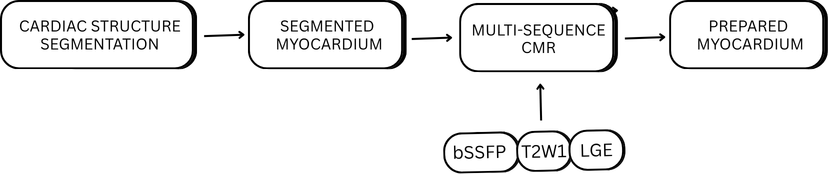
\includegraphics[width=0.86\textwidth]{bab3/ch3-prepared-myocardium.png}
	\caption{Preparation of the myocardium region for myocardial scar assessment}
	\label{fig:ch3-prepared-myocardium}
\end{figure}

\section{Myocardial Scar Assessment}
\label{sec:scar-assessment-method}

Following cardiac structure segmentation, the proposed framework proceeds to myocardial scar assessment using the MyoPS2020 dataset. The objective of this stage is to automatically identify myocardial scar from multi-sequence CMR images and subsequently estimate the corresponding myocardial scar area. Unlike the previous stage, which focuses on cardiac anatomy, this stage focuses on identifying pathological tissue within the segmented myocardium.

The segmented myocardium prepared in Section~\ref{subsec:scar-preparation} provides the anatomical information required for myocardial scar assessment. The corresponding multi-sequence CMR images are subsequently processed using a residual attention-based network to identify myocardial scar. The resulting scar segmentation is then converted into quantitative scar area measurements for myocardial infarction assessment. The overall workflow of this stage is illustrated in Figure~\ref{fig:ch3-scar-framework}.

\begin{figure}[htbp]
	\centering
	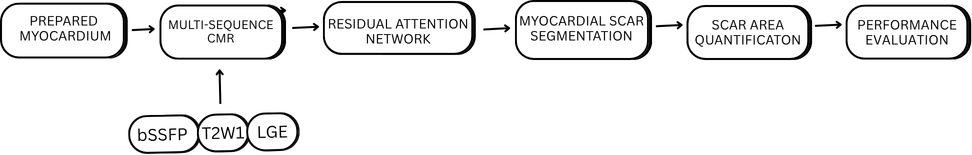
\includegraphics[width=0.86\textwidth]{bab3/ch3-scar-framework.png}
	\caption{Overview of the myocardial scar assessment framework}
	\label{fig:ch3-scar-framework}
\end{figure}

As illustrated in Figure~\ref{fig:ch3-scar-framework}, the prepared myocardium and the corresponding multi-sequence CMR images are processed by the residual attention network to identify myocardial scar. The resulting scar segmentation is subsequently converted into quantitative scar area measurements before being evaluated using the performance metrics described in Section~\ref{sec:performance-evaluation}.

\subsection{Multi-sequence Cardiac Magnetic Resonance Images}
\label{subsec:multi-sequence-method}

Myocardial scar assessment was performed using the MyoPS2020 dataset, which provides three complementary CMR image sequences, namely balanced steady-state free precession (bSSFP), T2-weighted imaging (T2WI), and Late Gadolinium Enhancement (LGE). Each image sequence provides different anatomical and pathological information, allowing the proposed framework to utilize complementary image characteristics during myocardial scar assessment \citep{Zhuang2020}.

Before myocardial scar assessment, the segmented myocardium obtained from the previous stage was associated with the corresponding multi-sequence CMR images. Next, the bSSFP, T2WI, and LGE images were prepared as the input for the proposed scar assessment framework. This preparation enables the network to analyze complementary information from the three CMR image sequences while maintaining their anatomical correspondence.

The overall preparation of the multi-sequence CMR images is illustrated in Figure~\ref{fig:ch3-multi-sequence-preparation}.

\begin{figure}[htbp]
	\centering
	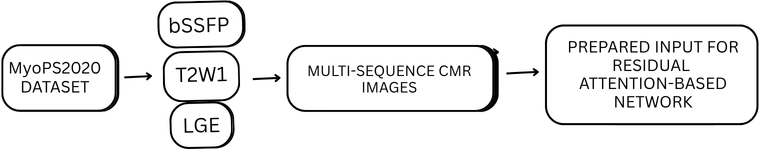
\includegraphics[width=0.86\textwidth]{bab3/ch3-multi-sequence-preparation.png}
	\caption{Preparation of multi-sequence CMR images for myocardial scar assessment}
	\label{fig:ch3-multi-sequence-preparation}
\end{figure}

As illustrated in Figure~\ref{fig:ch3-multi-sequence-preparation}, the three CMR image sequences are combined to provide complementary image information before being processed by the proposed myocardial scar assessment framework. The prepared images are subsequently analysed using the residual attention-based network described in the following section.

\subsection{Residual Attention Network}
\label{subsec:residual-attention-network}

The proposed myocardial scar assessment framework adopts a residual attention-based network to identify myocardial scar from multi-sequence CMR images. Compared with cardiac structure segmentation, myocardial scar exhibits greater variations in shape, size, and image intensity, making automatic segmentation more challenging \citep{He2016,Oktay2018}.

The network adopts an encoder--decoder architecture that integrates residual learning and attention mechanisms. Residual learning facilitates the extraction of image features across multiple network layers, while the attention mechanism guides the network to focus on image regions that are more relevant to myocardial scar. The prepared multi-sequence CMR images described in Section~\ref{subsec:multi-sequence-method} serve as the network input, whereas the corresponding scar annotations are used as the reference during network training.

The residual attention network generates a myocardial scar segmentation that is subsequently used for quantitative scar area estimation, as described in Section~\ref{subsec:scar-area}. The detailed implementation of the proposed network is presented in Chapter VI.

\subsection{Myocardial Scar Segmentation}
\label{subsec:scar-segmentation}

The residual attention network produces a pixel-level segmentation of myocardial scar within the myocardium region prepared in the previous stage. During network training, the predicted scar segmentation is compared with the corresponding reference annotation provided in the MyoPS2020 dataset, enabling the network to learn the spatial distribution of myocardial scar from multi-sequence CMR images \citep{Zhuang2020}.

To ensure that the analysis is focused on the pathological tissue of interest, myocardial scar segmentation is performed within the myocardium identified during the cardiac structure segmentation stage. The segmentation output is represented as a binary scar mask indicating the spatial distribution of myocardial scar within the myocardium.

The resulting scar segmentation serves as the basis for myocardial scar area quantification, which is described in Section~\ref{subsec:scar-area}. The implementation details and experimental evaluation of the proposed scar segmentation framework are presented in Chapter VI.

\subsection{Myocardial Scar Area Quantification}
\label{subsec:scar-area}

Following myocardial scar segmentation, the segmented scar region is converted into a quantitative measurement of myocardial scar area. Quantitative scar area measurement derived from segmentation results has been widely adopted in CMR image analysis to objectively estimate the extent of myocardial scar \citep{Karim2016,Zhuang2020}.

The myocardial scar area is calculated from the binary scar mask generated by the residual attention network. The total number of pixels classified as myocardial scar is first determined and subsequently converted into a physical area using the spatial resolution of the corresponding CMR image. The myocardial scar area is calculated as

\begin{equation}
A_{\mathrm{scar}} = N_{\mathrm{scar}} \times A_{\mathrm{pixel}}
\label{eq:scar-area}
\end{equation}

where $A_{\mathrm{scar}}$ denotes the estimated myocardial scar area (mm$^2$), $N_{\mathrm{scar}}$ is the total number of pixels classified as myocardial scar, and $A_{\mathrm{pixel}}$ represents the physical area corresponding to a single image pixel (mm$^2$/pixel).

The estimated myocardial scar area obtained from the proposed framework was subsequently compared with the corresponding reference measurements using MAE, RMSE, PCC, and Bland--Altman analysis, as described in Section~\ref{sec:performance-evaluation}.

\section{Experimental Design}
\label{sec:experimental-design}

The experimental design adopted in this dissertation was developed to systematically evaluate the contribution of each methodological component within the proposed deep learning framework for CMR image analysis. Rather than modifying several components simultaneously, each investigation focused on a single methodological component while maintaining the remaining experimental settings unchanged. This experimental strategy enables the influence of each investigated component to be evaluated independently and ensures that the observed performance differences are attributable to the investigated method.

As illustrated in Figure~\ref{fig:ch3-experimental-design}, the study was conducted through four sequential stages. A preliminary investigation was first performed to establish the baseline segmentation framework through activation function selection. Following this, the proposed framework was progressively developed through fuzzy pooling integration and loss function investigation before being applied to myocardial scar assessment and quantitative scar area estimation. The corresponding methodological components investigated at each stage are summarized in Table~\ref{tab:experimental-design}.

\begin{figure}[htbp]
\centering
\fbox{\parbox{0.86\textwidth}{\centering Insert final experimental design adopted in this study. here}}
\caption{Experimental design adopted in this study.}
\label{fig:ch3-experimental-design}
\end{figure}
%\noindent\textit{Source: Developed by the author.}

\begin{table}[htbp]
\centering
\caption{Overview of the experimental design adopted in this study}
\label{tab:experimental-design}
\begin{tabularx}{\textwidth}{
		>{\raggedright\arraybackslash}p{0.18\textwidth}
		>{\raggedright\arraybackslash}p{0.30\textwidth}
		>{\raggedright\arraybackslash}X
	}
	\toprule
	\textbf{Stage} & \textbf{Methodological Component} & \textbf{Purpose} \\
	\midrule
	Preliminary Study & Activation function selection & Establish the baseline segmentation framework \\
	Stage I & Fuzzy pooling integration & Investigate the influence of the pooling strategy on cardiac structure segmentation \\
	Stage II & Loss function investigation & Evaluate different loss functions for cardiac structure segmentation \\
	Stage III & Myocardial scar assessment & Perform myocardial scar segmentation and quantitative scar area estimation \\
	\bottomrule
\end{tabularx}
\end{table}
%\noindent\textit{Source: Developed by the author.}

As summarized in Figure~\ref{fig:ch3-experimental-design} and Table~\ref{tab:experimental-design}, the proposed framework was developed progressively, where the outcome of each stage served as the basis for the subsequent investigation. This experimental design ensures methodological consistency throughout the dissertation while enabling each investigated component to be evaluated independently.

\section{Performance Evaluation}
\label{sec:performance-evaluation}

The proposed framework was evaluated using quantitative performance metrics selected according to the objective of each stage of the study. Since this dissertation consists of cardiac structure segmentation, myocardial scar segmentation, and myocardial scar area quantification, different evaluation metrics were adopted to assess segmentation accuracy, boundary agreement, structural similarity, and quantitative measurement agreement. The mathematical formulations of these metrics have been presented in Chapter~\ref{chap:2}, whereas their application in this study is summarized in Table~\ref{tab:evaluation-metrics}.

\begin{sidewaystable}[htbp]
	\centering
	\small
	\caption{Performance evaluation metrics adopted in this study}
	\label{tab:evaluation-metrics}
	
	\renewcommand{\arraystretch}{1.3}
	\begin{tabularx}{\linewidth}{>{\raggedright\arraybackslash}p{0.20\linewidth} >{\raggedright\arraybackslash}p{0.20\linewidth} p{0.12\linewidth} >{\raggedright\arraybackslash}X}
		\toprule
		\textbf{Task} & \textbf{Output} & \textbf{Metric} & \textbf{Purpose} \\ \midrule
		
		Cardiac structure segmentation & 
		LV, RV, and myocardium & 
		IoU \newline HD & 
		Measure regional agreement \newline Assess boundary accuracy \\ \addlinespace % <-- Diganti ke \addlinespace
		
		Myocardial scar segmentation & 
		Myocardial scar segmentation & 
		DSC \newline IoU \newline HD \newline SSIM & 
		Evaluate segmentation overlap \newline Measure regional agreement \newline Assess boundary accuracy \newline Evaluate structural similarity \\ \addlinespace % <-- Diganti ke \addlinespace
		
		Myocardial scar area quantification & 
		Myocardial scar area (mm$^2$) & 
		MAE \newline RMSE \newline PCC \newline Bland--Altman & 
		Measure absolute estimation error \newline Measure the magnitude of estimation error while penalizing larger errors \newline Evaluate measurement correlation \newline Assess agreement between estimated and reference scar area \\ \bottomrule
	\end{tabularx}
\end{sidewaystable}

As summarized in Table~\ref{tab:evaluation-metrics}, segmentation performance was evaluated using overlap-based, boundary-based, and structural similarity metrics, whereas myocardial scar area quantification was evaluated using quantitative agreement analysis. The detailed experimental results obtained using these evaluation metrics are presented in Chapters IV, V, and VI.
		%\cleardoublepage
		\clearpage
		
		\chapter{CARDIAC STRUCTURE SEGMENTATION USING AN ENHANCED U-NET WITH FUZZY POOLING}
\label{chap:4}

\section{Overview}
\label{sec:ch4-intro-overview}

This chapter presents the development and evaluation of the proposed cardiac structure segmentation framework, which constitutes the first stage of the deep learning framework for myocardial infarction assessment developed in this dissertation. Specifically, this chapter investigates the effects of activation function selection and fuzzy pooling layer configuration on cardiac structure segmentation performance using cine cardiac magnetic resonance images. The resulting anatomical representations provide the foundation for the subsequent investigation of myocardium segmentation and myocardial scar assessment presented in the following chapters.

Cardiovascular disease remains one of the leading causes of mortality worldwide and continues to impose a substantial clinical and socioeconomic burden despite significant advances in diagnostic and therapeutic technologies \citep{Tsao2022,WHO2021}. Accurate assessment of cardiac morphology and function is therefore essential for early diagnosis, treatment planning, and long-term monitoring of patients with various cardiovascular disorders. Among available imaging modalities, CMR has become the clinical reference standard because it provides high spatial resolution, excellent soft tissue contrast, and comprehensive visualization of cardiac anatomy and ventricular function without ionizing radiation \citep{Agrawal2020}.

Quantitative clinical parameters derived from CMR, including ventricular volume, myocardial mass, stroke volume, and ejection fraction, are obtained through the segmentation of the left ventricle (LV), right ventricle (RV), and myocardium (MYO) across the cardiac cycle. Consequently, accurate segmentation of these anatomical structures constitutes a fundamental prerequisite for reliable functional assessment and subsequent diagnosis. Any segmentation inaccuracies directly propagate into quantitative measurements, potentially affecting clinical interpretation and therapeutic decision-making \citep{Petitjean2011,Bernard2018}.

Although manual segmentation remains the clinical reference standard, numerous CMR image segmentation methods have been proposed to improve accuracy, efficiency, and reproducibility \citep{Petitjean2011}.

Recent advances in deep learning have substantially improved automatic medical image segmentation. Among various convolutional neural network architectures, U-Net has become one of the most widely adopted frameworks because its encoder--decoder structure, combined with skip connections, effectively integrates semantic information and fine spatial details, enabling accurate localization even with relatively limited annotated medical datasets \citep{Ronneberger2015,Siddique2021}. Consequently, numerous CMR image segmentation methods have been developed to overcome these limitations using deep learning techniques \citep{Ronneberger2015,Siddique2021}.

Despite its widespread success, the segmentation accuracy of conventional U-Net remains influenced by several architectural components. One critical component is the pooling operation applied during the encoder pathway. Conventional max pooling reduces feature-map resolution by retaining only the maximum activation within each pooling region. While this strategy effectively enlarges the receptive field and decreases computational complexity, repeated application may discard weaker activations that still contain important anatomical information, particularly around thin myocardial boundaries and low-contrast tissue interfaces \citep{Nirthika2022,Diamantis2020}. Such information loss may reduce boundary precision and adversely affect the delineation of anatomically complex cardiac structures.

Several alternative pooling strategies have therefore been proposed to preserve richer spatial representations during feature aggregation. Among these approaches, fuzzy pooling introduces fuzzy membership concepts to aggregate information from multiple activations rather than relying solely on the strongest response. By incorporating weighted contributions from neighboring activations, fuzzy pooling is expected to preserve local contextual information more effectively while reducing sensitivity to minor image variations and noise \citep{Diamantis2020}. Nevertheless, its effectiveness for multi-structure cardiac segmentation using cine cardiac MRI has not been comprehensively investigated.

Based on this research gap, this chapter develops an enhanced cardiac structure segmentation framework by integrating fuzzy pooling into the encoder pathway of the conventional U-Net architecture. Rather than introducing a completely new segmentation network, this study investigates whether improving the feature aggregation mechanism during down-sampling can preserve richer anatomical information and consequently improve the segmentation performance of the left ventricle (LV), right ventricle (RV), and myocardium (MYO) throughout the cardiac cycle.

The proposed framework is implemented using cine cardiac MRI obtained from the Automated Cardiac Diagnosis Challenge (ACDC) dataset. To ensure that the observed performance differences originate from the investigated pooling mechanism, the network architecture, activation function, optimizer, learning rate, training protocol, and evaluation metrics were maintained consistently across the experiments; the batch size followed the source-study configuration for each pooling strategy. Consequently, fuzzy pooling becomes the only architectural component evaluated against the conventional max pooling strategy under controlled experimental conditions.

The performance of the proposed framework is quantitatively evaluated using Intersection over Union (IoU) and Hausdorff Distance (HD), while qualitative assessment is performed through visual comparison of the generated segmentation masks. Furthermore, the experimental findings are analyzed to determine how feature preservation during the down-sampling process influences segmentation accuracy, boundary delineation, and anatomical consistency of cardiac structures.

This chapter presents an enhanced U-Net framework for cardiac structure segmentation by incorporating fuzzy pooling into the feature extraction process. The proposed modification aims to preserve richer anatomical information during down-sampling while maintaining the simplicity of the original U-Net architecture. The effectiveness of the proposed framework is evaluated through quantitative and qualitative analyses using cine cardiac MRI datasets. The enhanced cardiac structure segmentation established in this chapter subsequently provides the anatomical myocardium representation required for the investigations presented in Chapter V and Chapter VI.

\section{Proposed Cardiac Structure Segmentation Framework}
\label{sec:ch4-framework}

This chapter develops a cardiac structure segmentation framework by enhancing the conventional U-Net architecture with fuzzy pooling to improve cardiac structure segmentation through improved anatomical feature representation during encoder down-sampling. Rather than proposing a new segmentation network, this study investigates whether improving the feature aggregation mechanism alone is sufficient to enhance the delineation of the left ventricle, right ventricle, and myocardium from cine cardiac MRI.

As described in Chapter III, pooling operation is one of the architectural components that directly influences the quality of hierarchical feature representations learned by a convolutional neural network. Since all subsequent decoding and boundary reconstruction processes depend on the encoded feature maps, excessive information loss during down-sampling may propagate throughout the network and ultimately reduce segmentation accuracy. Therefore, this study focuses on improving feature aggregation during pooling while preserving the overall network architecture.

Accordingly, the proposed framework applies the original U-Net architecture as the segmentation backbone and replaces the conventional max pooling operation with fuzzy pooling in the encoder pathway. This modification aims to preserve richer anatomical information during feature down-sampling without altering the encoder--decoder topology, skip connections, or training strategy. Consequently, any performance differences observed in the experimental evaluation can be primarily attributed to the investigated pooling mechanism rather than to changes in network complexity or architectural design.

Figure~\ref{fig:ch4-workflow} illustrates the overall workflow of the proposed cardiac structure segmentation framework. Beginning with cine cardiac MRI acquisition, the framework performs image preprocessing, feature extraction using the enhanced U-Net architecture, cardiac structure segmentation, and quantitative performance evaluation.

\begin{figure}[htbp]
	\centering
	\fbox{\parbox{0.86\textwidth}{\centering Insert Overall workflow of the proposed enhanced U-Net framework for cardiac structure segmentation here}}
	\caption{Overall workflow of the proposed enhanced U-Net framework for cardiac structure segmentation}
	\label{fig:ch4-workflow}
\end{figure}
%\noindent\textit{Source: Author's illustration based on the proposed framework.}

As illustrated in Figure~\ref{fig:ch4-workflow}, cine cardiac MRI images are first preprocessed through image resizing and normalization before being forwarded into the segmentation network. The encoder progressively extracts hierarchical anatomical features while reducing spatial resolution. Unlike the conventional U-Net, each down-sampling stage incorporates fuzzy pooling to preserve contextual information that may otherwise be discarded during feature aggregation. The decoder subsequently reconstructs the segmentation masks by combining semantic representations from deeper layers with fine spatial information transferred through skip connections. The final output consists of pixel-wise segmentation masks corresponding to the left ventricle, right ventricle, and myocardium. These segmentation results are then quantitatively evaluated using IoU and HD.

The following sections describe each component of the proposed framework in greater detail.

\subsection{Baseline U-Net Architecture}
\label{subsec:ch4-unet}

U-Net has become one of the most widely adopted convolutional neural network architectures for cardiac structure segmentation because of its encoder--decoder design, which effectively combines high-level contextual information with fine spatial details through skip connections \citep{Ronneberger2015}. Unlike conventional convolutional neural networks designed primarily for image classification, U-Net performs dense pixel-wise prediction by integrating contextual information from multiple spatial resolutions through its encoder--decoder architecture.

The encoder gradually extracts increasingly abstract feature representations while reducing spatial resolution, enabling the network to learn high-level semantic information. Conversely, the decoder progressively restores the original image resolution and reconstructs the segmentation mask. Skip connections directly transfer fine-grained spatial information from corresponding encoder layers to decoder layers, allowing the network to recover anatomical details that may otherwise be lost during feature compression. This architectural characteristic has made U-Net one of the most successful frameworks for medical image segmentation involving complex anatomical structures with varying sizes and shapes.

The selection of U-Net in this study is further motivated by its extensive application in cardiac MRI segmentation. Previous studies have demonstrated that U-Net provides reliable segmentation of ventricular cavities and myocardial structures while maintaining relatively simple network complexity and efficient training characteristics. These advantages make U-Net an appropriate baseline architecture for investigating architectural modifications intended to improve segmentation performance without introducing additional sources of variation.

Despite these advantages, one limitation of the conventional U-Net lies in its use of max pooling throughout the encoder pathway. During each down-sampling operation, max pooling retains only the strongest activation within a local neighborhood while discarding all remaining responses. Although this mechanism effectively reduces computational complexity and enlarges the receptive field, repeated application may eliminate weaker activations that still contain meaningful anatomical information, particularly around thin myocardial boundaries or regions exhibiting subtle intensity variations \citep{Nirthika2022,Diamantis2020}.

For cardiac MRI segmentation, preserving these weak yet informative responses is particularly important because the myocardium often appears as a relatively thin ring-shaped structure whose boundaries exhibit gradual intensity transitions rather than sharp edges. Consequently, the accumulated information loss introduced by repeated max pooling may reduce boundary precision and anatomical consistency in the final segmentation masks.

Instead of redesigning the overall network architecture, this study addresses this limitation by replacing only the pooling operation while maintaining all other architectural components unchanged. This strategy enables a direct investigation of the influence of pooling mechanisms on cardiac structure segmentation performance under controlled experimental conditions.

\subsection{Activation Function Selection}
\label{subsec:ch4-activation}

The activation function used throughout the proposed framework was determined based on the preliminary investigation presented in the preceding stage of this dissertation. The earlier study systematically compared several activation functions for multi-structure cardiac MRI segmentation and demonstrated that the Rectified Linear Unit (ReLU) consistently achieved superior segmentation performance compared with the Mish activation function under the same experimental settings.

The selection of ReLU is supported not only by its computational simplicity but also by its ability to alleviate the vanishing gradient problem, thereby facilitating stable training during deep network training \citep{Nair2010}. Moreover, its sparse activation characteristic allows efficient feature learning while maintaining stable convergence throughout the training process.

Since the objective of this chapter is to investigate the effect of pooling mechanisms rather than activation functions, ReLU is consistently used in every experiment to eliminate activation function variability as a potential confounding factor. Consequently, all comparative analyses presented in this chapter are performed using identical activation functions, ensuring that the observed performance differences originate solely from the investigated pooling strategy.

\subsection{Integration of Fuzzy Pooling}
\label{subsec:ch4-fuzzy}

The principal contribution of this chapter is the development of an enhanced cardiac structure segmentation framework through the integration of fuzzy pooling into the encoder pathway of the U-Net architecture. Rather than introducing a completely new network architecture, this study investigates whether improving the feature aggregation mechanism during down-sampling can strengthen anatomical feature preservation and subsequently improve cardiac structure segmentation performance of the left ventricle (LV), right ventricle (RV), and myocardium (MYO).

The motivation for this architectural modification arises from one of the inherent limitations of conventional U-Net. During feature extraction, every encoder stage performs spatial down-sampling using max pooling to reduce computational complexity while enlarging the receptive field. Although this operation efficiently preserves the strongest feature response within each local neighborhood, all remaining activations are discarded. Repeated application of this operation throughout multiple encoder levels may progressively eliminate weak but anatomically meaningful responses that contribute to tissue continuity and boundary definition \citep{Nirthika2022}.

This limitation becomes particularly important for cine cardiac MRI because ventricular boundaries and myocardial tissues are often characterized by gradual intensity transitions and relatively thin anatomical structures. Consequently, weak feature responses discarded during repeated max pooling may correspond to clinically meaningful anatomical information.

Instead of redesigning the entire segmentation network, this study addresses the problem at its source by improving the feature aggregation process itself. The proposed framework replaces every max pooling layer in the encoder with fuzzy pooling while preserving the overall U-Net architecture, including the encoder--decoder topology, skip connections, convolutional blocks, and decoding pathway. As a result, the overall learning capacity of the network remains comparable to the baseline model, allowing the influence of the pooling mechanism to be evaluated independently without introducing additional architectural complexity.

To clearly illustrate the architectural modification introduced in this study, Figure~\ref{fig:ch4-fuzzy-integration} presents the integration of fuzzy pooling within the encoder pathway of the proposed enhanced U-Net framework. The figure highlights that only the pooling operation is replaced, whereas the encoder--decoder topology, skip connections, convolutional blocks, and decoder remain identical to the baseline architecture. This visualization emphasizes that the proposed framework isolates the effect of the pooling mechanism without introducing additional architectural complexity.

\begin{figure}[htbp]
	\centering
	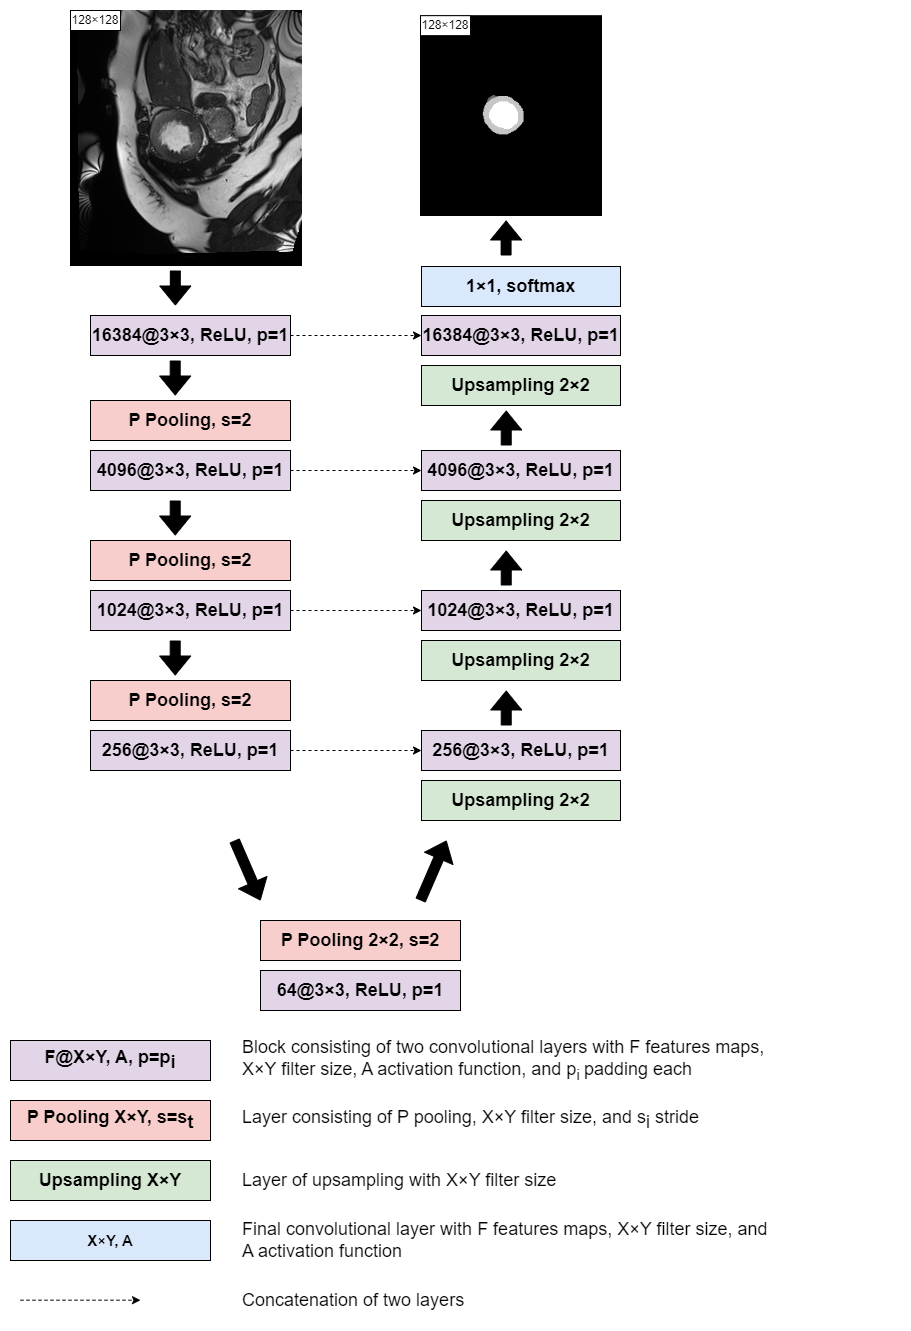
\includegraphics[width=0.86\textwidth]{bab4/ch4-fuzzy-integration.png}
	\caption{Integration of fuzzy pooling within the encoder of the proposed enhanced U-Net framework \citep{Riandini2023MeMeA}}
	\label{fig:ch4-fuzzy-integration}
\end{figure}

As shown in Figure~\ref{fig:ch4-fuzzy-integration}, each convolutional block is followed by a ReLU activation layer before entering the fuzzy pooling module. The resulting feature maps are subsequently propagated to deeper encoder levels while corresponding high-resolution features are preserved through skip connections and later combined during decoder reconstruction. Since only the pooling operation is modified, all remaining components of the segmentation network remain identical to those of the baseline U-Net. This architectural consistency establishes a controlled experimental setting in which the effect of fuzzy pooling can be directly observed.

While Figure~\ref{fig:ch4-fuzzy-integration} illustrates where fuzzy pooling is incorporated within the network architecture, Figure~\ref{fig:ch4-pooling-comparison} explains how the pooling operation aggregates feature responses during encoder down-sampling. This conceptual illustration facilitates understanding of the difference between conventional max pooling and fuzzy pooling before the mathematical formulation of the proposed pooling operation is introduced.

\begin{figure}[htbp]
	\centering
	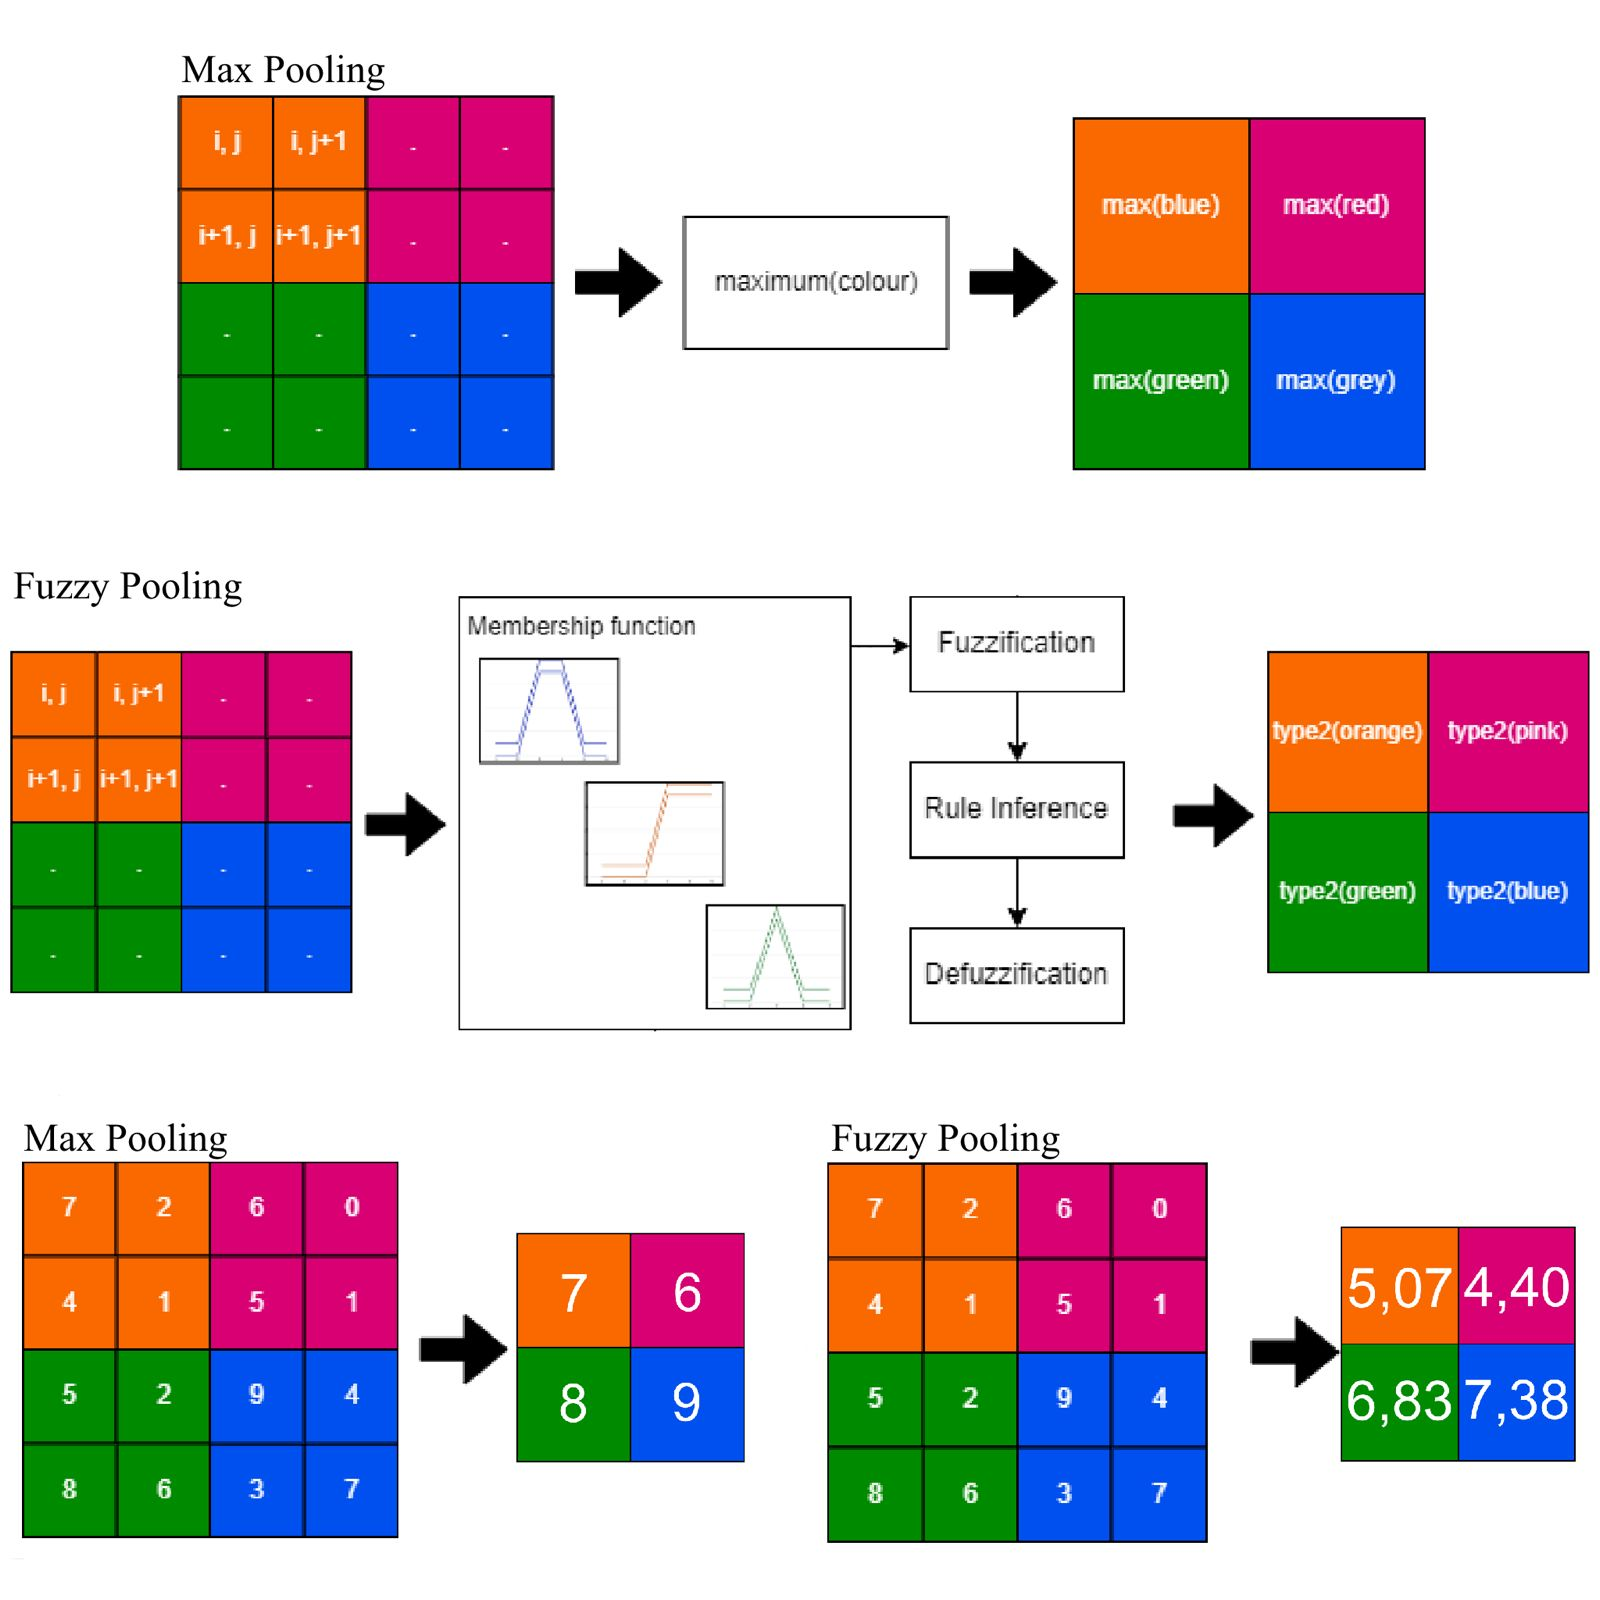
\includegraphics[width=0.86\textwidth]{bab4/ch4-pooling-comparison.png}
	\caption{Illustration of comparison between conventional max pooling and the proposed fuzzy pooling operation \citep{Riandini2023MeMeA}}
	\label{fig:ch4-pooling-comparison}
\end{figure}

Unlike conventional max pooling, which represents an entire pooling region using only its maximum activation, fuzzy pooling evaluates the contribution of every activation within the pooling window through fuzzy membership functions. Instead of selecting a single dominant response, the pooled representation is obtained from the weighted contribution of all neighboring activations according to their relative importance. Consequently, feature aggregation becomes more representative of the local anatomical context rather than depending exclusively on the strongest response.

Based on the feature aggregation mechanism illustrated in Figure~\ref{fig:ch4-pooling-comparison}, the fuzzy pooling operation computes the pooled representation as a weighted combination of all feature responses within the pooling window. The mathematical formulation of the proposed pooling strategy is given by Equation~\eqref{eq:ch4-fuzzy}.

\begin{equation}
	P_{\mathrm{fuzzy}}
	=
	\frac{\sum_{i=1}^{n}\mu_i x_i}
	{\sum_{i=1}^{n}\mu_i}
	\label{eq:ch4-fuzzy}
\end{equation}

where \(x_i\) represents the activation value within the pooling region and \(\mu_i\) denotes its corresponding fuzzy membership coefficient. Unlike max pooling, which ignores all non-maximum activations, this formulation allows informative responses with lower activation values to continue contributing to the encoded feature representation.

From a medical imaging perspective, this characteristic is particularly advantageous for cardiac MRI segmentation. Anatomical boundaries are rarely represented by isolated high-intensity responses; instead, they emerge from spatially correlated intensity transitions distributed across neighboring pixels. By preserving these distributed responses during successive down-sampling operations, fuzzy pooling enables the encoder to retain richer structural information describing ventricular cavities and myocardial boundaries. The decoder subsequently exploits these preserved representations to reconstruct segmentation masks with improved anatomical continuity.

It should be emphasized that the objective of this modification is not to increase network complexity, but rather to improve the quality of hierarchical feature representations learned throughout the encoding process. Therefore, the scientific contribution of this study lies in demonstrating that a relatively simple modification to the feature aggregation mechanism can substantially improve cardiac structure segmentation without requiring additional encoder branches, attention modules, or more complex network architectures.

Collectively, the integration of fuzzy pooling enables improved anatomical feature representation while preserving the original U-Net architecture. This enhanced segmentation framework is subsequently evaluated using the experimental protocol described in the following section.

\section{Materials and Experimental Setup}
\label{sec:ch4-materials}

To objectively evaluate the proposed cardiac structure segmentation framework, a controlled experimental protocol was established to ensure that the observed performance differences originated solely from the investigated pooling mechanism. Accordingly, all comparative models utilized the same dataset, preprocessing procedures, training strategy, and evaluation protocol, thereby enabling the effectiveness of the proposed cardiac structure segmentation framework to be objectively evaluated under controlled and reproducible conditions.

The following subsections describe the dataset, computational environment, training configuration, and evaluation metrics adopted to validate the proposed framework.

\subsection{Dataset}
\label{subsec:ch4-dataset}

The proposed framework was evaluated using the Automated Cardiac Diagnosis Challenge (ACDC) 2017 dataset, one of the most widely adopted public benchmarks for CMR segmentation. The dataset was selected because it provides expert-annotated segmentation masks for the left ventricle (LV), right ventricle (RV), and myocardium (MYO), enabling objective and reproducible evaluation of multi-structure cardiac segmentation algorithms. In addition, the inclusion of multiple cardiac pathologies provides substantial anatomical variability, allowing the robustness of the proposed framework to be assessed under clinically diverse conditions.

The ACDC dataset consists of cine cardiac MRI examinations acquired from 150 patients representing five clinical groups, namely normal subjects, previous myocardial infarction, dilated cardiomyopathy, hypertrophic cardiomyopathy, and abnormal right ventricle. Each examination contains short-axis cine MRI slices covering the cardiac cycle, together with expert manual annotations for the LV, RV, and MYO at the End-Diastole (ED) and End-Systole (ES) phases. These expert annotations serve as the reference standard for supervised training and quantitative evaluation.

Following the experimental protocol adopted in the source study, the dataset was divided into 100 patients for training and 50 patients for testing, resulting in 1,616 training images and 286 testing images after extracting the ED and ES frames from each examination. Using identical data partitions throughout all comparative experiments eliminates dataset-related variability and ensures that the observed performance differences originate from the investigated pooling mechanism rather than differences in data distribution.

Prior to network training, all images were resized to 128 $\times$ 128 pixels while preserving the complete anatomical field of view through image resampling. Pixel intensity normalization was subsequently applied to reduce intensity variation among examinations and to facilitate stable training during network training. The same preprocessing pipeline was consistently applied to all comparative models to ensure fair and reproducible performance evaluation.

\subsection{Experimental Environment}
\label{subsec:ch4-environment}

To ensure reproducibility and experimental consistency, all comparative experiments were conducted under an identical computational environment. Maintaining the same hardware platform, software implementation, preprocessing pipeline, and inference procedure minimizes external sources of variability and ensures that any observed performance differences can be attributed exclusively to the investigated pooling mechanism.

Both the baseline U-Net and the proposed enhanced U-Net were implemented using the Python programming language together with established deep learning libraries for medical image analysis. Model training was performed on a Graphics Processing Unit (GPU), enabling efficient selection of the encoder--decoder architecture and reducing computational time during iterative training.

Throughout the experimental study, the computational environment remained unchanged for all comparative models. Consequently, hardware configuration, software implementation, preprocessing procedures, and inference settings were identical across all experiments. This controlled experimental environment provides a fair basis for comparing the conventional max pooling strategy with the proposed fuzzy pooling approach, ensuring that the reported improvements reflect the effectiveness of the proposed feature aggregation mechanism rather than differences in implementation or computational resources.

\subsection{Training Configuration}
\label{subsec:ch4-training}

A controlled training strategy was adopted to isolate the influence of the pooling mechanism from other selection factors. Therefore, all comparative models utilized the same network architecture, activation function, optimizer, learning rate, training protocol, and stopping criteria. The only architectural modification introduced in this study was the replacement of the conventional max pooling layers with fuzzy pooling throughout the encoder pathway. This controlled configuration ensures that the contribution of fuzzy pooling can be evaluated independently without interference from other training variables.

Except for the batch size required by each pooling strategy, all remaining experimental settings were maintained consistently to ensure a fair comparison between the investigated pooling methods.

The complete experimental settings adopted throughout this study are summarized in Table~\ref{tab:ch4-training}.

\begin{table}[htbp]
	\centering
	\caption{Training configuration}
	\label{tab:ch4-training}
	\begin{tabularx}{0.88\textwidth}{p{0.30\textwidth} X}
		\toprule
		\textbf{Parameter} & \textbf{Configuration} \\
		\midrule
		Dataset & ACDC \\
		Input size & $128 \times 128$ pixels \\
		Activation function & ReLU \\
		Optimizer & Adam \\
		Learning rate & 0.0001 \\
		Batch size & 8 (max pooling); 4 (fuzzy pooling) \\
		Loss function & Categorical cross-entropy \\
		Evaluation metrics & IoU and HD \\
		\bottomrule
	\end{tabularx}
\end{table}

As summarized in Table~\ref{tab:ch4-training}, the principal model and training settings were maintained consistently, except for the batch size specified for each pooling strategy. Consequently, the pooling mechanism remained the principal architectural variable, allowing the observed performance differences to be attributed directly to the proposed fuzzy pooling strategy.

The ReLU activation function was consistently applied throughout all experiments based on the findings of the preliminary investigation presented in the previous chapter. Maintaining the same activation function eliminates selection variability associated with nonlinear feature transformation and ensures that the observed performance differences originate from the investigated pooling mechanism.

\subsection{Evaluation Metrics}
\label{subsec:ch4-metrics}

The segmentation performance of the proposed framework was evaluated using IoU and HD. IoU was used to evaluate the agreement between the predicted segmentation and the corresponding ground-truth annotation, whereas HD was used to assess boundary localization accuracy. The combination of these complementary metrics enables simultaneous evaluation of regional overlap and anatomical contour preservation, both of which are essential for reliable cardiac structure segmentation.

To quantitatively measure the overlap between the predicted segmentation and the corresponding ground-truth annotation, the IoU is computed according to Equation~\eqref{eq:ch4-iou}.

\begin{equation}
	\mathrm{IoU}(P,G)
	=
	\frac{|P\cap G|}{|P\cup G|}
	\label{eq:ch4-iou}
\end{equation}

where \(P\) and \(G\) denote the predicted and reference segmentation regions, respectively.

Although IoU effectively evaluates regional agreement, it does not explicitly measure boundary accuracy. Therefore, HD was additionally used to quantify the maximum distance between the predicted contour and the corresponding ground-truth contour.

Since regional overlap alone cannot fully describe segmentation quality, boundary localization accuracy is further evaluated using the HD, which measures the largest boundary discrepancy between the predicted segmentation and the ground truth. The HD is defined as Equation~\eqref{eq:ch4-hd}.

\begin{equation}
	\mathrm{HD}(P,G)
	=
	\max
	\left(
	\max_{p\in P}\min_{g\in G} d(p,g),
	\;
	\max_{g\in G}\min_{p\in P} d(g,p)
	\right)
	\label{eq:ch4-hd}
\end{equation}

where \(P\) and \(G\) represent the sets of boundary points of the predicted and ground-truth segmentations, respectively, and \(d(\cdot,\cdot)\) denotes the Euclidean distance between two boundary points. 

Using both metrics simultaneously enables segmentation performance to be assessed from complementary perspectives. A higher IoU indicates greater agreement between the predicted and reference regions, whereas a lower HD reflects better boundary agreement between the predicted segmentation and the reference. Since reliable segmentation of ventricular and myocardial boundaries is essential for subsequent quantitative cardiac analysis, the combined use of these metrics provides a more comprehensive evaluation of the proposed framework than either metric alone.

The experimental configuration can be summarized as follows:

\begin{itemize}
	\item \textbf{Dataset:} ACDC cine cardiac MRI dataset.
	\item \textbf{Input image size:} $128 \times 128$ pixels.
	\item \textbf{Segmented structures:} LV, RV, and MYO.
	\item \textbf{Optimizer:} Adam.
	\item \textbf{Evaluation metrics:} IoU and HD.
\end{itemize}

To further investigate the robustness of the proposed framework, all evaluations were performed independently for the End-Diastole (ED) and End-Systole (ES) phases. These two phases exhibit substantially different ventricular morphology and therefore present different levels of segmentation difficulty. Evaluating the proposed framework under both conditions enables a more rigorous assessment of its ability to preserve anatomical structures throughout the cardiac cycle.

\section{Experimental Results and Discussion}
\label{sec:ch4-results}

The effectiveness of the proposed cardiac structure segmentation framework was evaluated through a series of controlled experiments using the ACDC benchmark dataset. As described in Section~\ref{sec:ch4-materials}, all comparative models were developed under controlled experimental conditions, including the dataset, preprocessing pipeline, network architecture, activation function, training strategy, and evaluation protocol. Consequently, the pooling mechanism constituted the principal architectural variable, while the batch size followed the source-study configuration, allowing its contribution to segmentation performance to be objectively assessed.

To provide a comprehensive evaluation, the experimental findings are analyzed from four complementary perspectives. First, the training behaviour of the proposed framework is examined through the learning curves obtained during network training. Second, quantitative segmentation performance is evaluated using the IoU and HD. Third, qualitative comparisons are performed to assess the anatomical consistency of the generated segmentation masks. Finally, the overall findings are synthesized to explain the scientific contribution of the proposed framework and its implication for the subsequent stage of this research.

\subsection{Training Behaviour Analysis}
\label{subsec:ch4-training-behaviour}

Before evaluating the final segmentation accuracy, the convergence behaviour of the proposed framework was first examined to determine whether the integration of fuzzy pooling influences the learning process. Stable convergence indicates that the network is capable of learning representative feature patterns while maintaining good generalization to unseen data, whereas a large discrepancy between the training and validation losses may indicate overfitting. Therefore, analysing the learning behaviour provides an initial assessment of the effectiveness of the proposed feature aggregation strategy. The corresponding training and validation loss curves obtained during the training process are presented in Figure~\ref{fig:ch4-loss-curves}.

\begin{figure}[htbp]
	\centering
	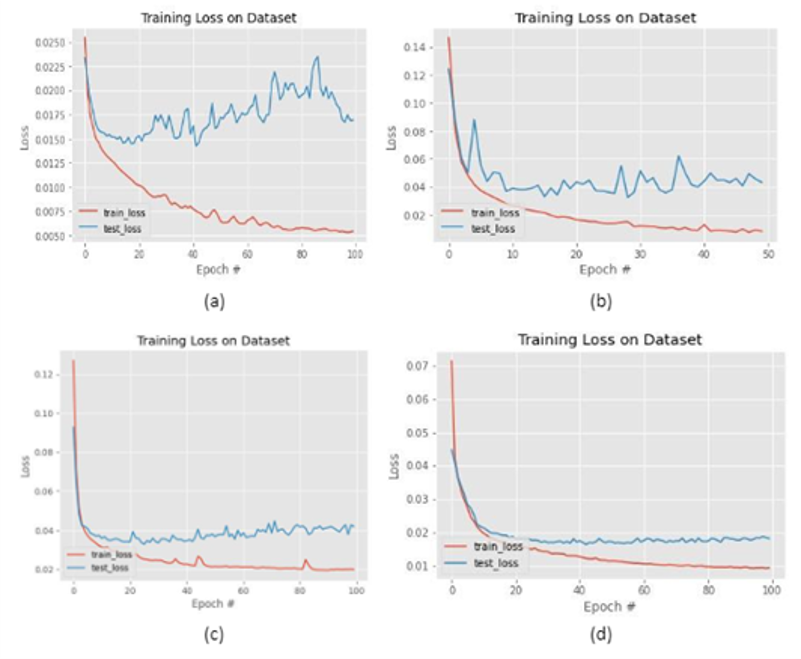
\includegraphics[width=0.86\textwidth]{bab4/ch4-loss-curves.png}
	\caption{Training and validation loss curves obtained using different pooling mechanisms and loss functions \citep{Riandini2023MeMeA}}
	\label{fig:ch4-loss-curves}
\end{figure}

Figure~\ref{fig:ch4-loss-curves} shows that all models successfully converged during the training process. Nevertheless, noticeable differences can be observed between the conventional U-Net adopting max pooling and the proposed framework incorporating fuzzy pooling, particularly for the multi-class segmentation task.

For the model using conventional max pooling with categorical cross-entropy, the training loss decreases rapidly, whereas the validation loss remains consistently higher throughout the training process. The relatively large gap between the two curves indicates that the learned feature representations are more strongly adapted to the training data, thereby reducing the model's ability to generalize to previously unseen cardiac MRI images.

In contrast, the proposed framework adopting fuzzy pooling demonstrates a more stable training behaviour. The training and validation losses decrease simultaneously with a noticeably smaller separation between the two curves, indicating that the learned feature representations are more robust and less sensitive to variations between the training and testing data. This behaviour suggests that preserving richer contextual information during feature aggregation contributes to a more effective learning process.

The convergence patterns observed in Figure~\ref{fig:ch4-loss-curves} are further supported by the final loss values summarized in Table~\ref{tab:ch4-loss}. While the learning curves provide a visual representation of the training process, the numerical results facilitate a more objective comparison between the conventional max pooling and the proposed fuzzy pooling strategies.

\begin{table}[htbp]
	\centering
	\caption{Final loss values obtained using different pooling mechanisms and loss functions}
	\label{tab:ch4-loss}
	\begin{tabular}{l l c}
		\toprule
		\textbf{Pooling mechanism} & \textbf{Loss function} & \textbf{Final loss} \\
		\midrule
		Max pooling & Binary cross-entropy & 0.01783 \\
		Fuzzy pooling & Binary cross-entropy & 0.04680 \\
		Max pooling & Categorical cross-entropy & 0.03596 \\
		Fuzzy pooling & Categorical cross-entropy & 0.03225 \\
		\bottomrule
		\multicolumn{3}{@{}l}{\vspace{4pt}\footnotesize \textit{Source:} Adapted from \citet{Riandini2023MeMeA}.}
	\end{tabular}
\end{table}

As summarized in Table~\ref{tab:ch4-loss}, the effectiveness of the pooling mechanism depends on the segmentation objective. For binary segmentation using binary cross-entropy, the conventional max pooling model achieved a lower loss value (0.01783) than the fuzzy pooling model (0.04680).

A different trend is observed for multi-class segmentation using categorical cross-entropy, which represents the primary objective of this study. The proposed fuzzy pooling model achieved a lower loss value (0.03225) than the conventional max pooling model (0.03596). This corresponds to a reduction of 0.00371, or approximately 10.3\%, indicating that the proposed framework learns more representative feature distributions for multi-class cardiac structure segmentation than the baseline architecture.

Although the numerical reduction appears relatively small, its scientific significance should be interpreted within the context of the experimental design. Both models were trained using identical datasets, preprocessing procedures, activation functions, training algorithms, and learning rates. Therefore, the lower loss obtained by the proposed framework can reasonably be attributed to the integration of fuzzy pooling rather than differences in training settings or network architecture.

The improved training performance can be attributed to the feature aggregation mechanism introduced by fuzzy pooling. Unlike conventional max pooling, which preserves only the strongest activation within each pooling region, fuzzy pooling aggregates information from multiple neighboring activations according to their relative contributions. Consequently, richer contextual information is retained during encoder down-sampling, enabling the network to learn more representative anatomical features.

Overall, the training behaviour analysis demonstrates that integrating fuzzy pooling contributes to more stable convergence and improved feature learning during network training. The agreement between the learning curves and the final loss values indicates that the proposed framework learns more representative anatomical features, which subsequently lead to improved cardiac structure segmentation performance. The quantitative segmentation results are presented in the following subsection.

\subsection{Quantitative Segmentation Performance}
\label{subsec:ch4-quantitative}

The effectiveness of the proposed cardiac structure segmentation framework was quantitatively evaluated using two complementary metrics, namely IoU and HD. IoU measures the degree of overlap between the predicted segmentation and the manually annotated reference, whereas HD evaluates the maximum boundary discrepancy between the corresponding contours. Evaluating both metrics simultaneously provides a comprehensive assessment of segmentation quality because reliable cardiac structure segmentation requires not only accurate region identification but also precise anatomical boundary delineation.

The quantitative comparison between the conventional U-Net using max pooling and the proposed enhanced U-Net incorporating fuzzy pooling is presented in Table~\ref{tab:ch4-performance}.

\begin{table}[htbp]
	\centering
	\caption{Quantitative comparison between max pooling and fuzzy pooling}
	\label{tab:ch4-performance}
	\begin{tabular}{l c c c c}
		\toprule
		\textbf{Pooling} & \textbf{IoU ED (\%)} & \textbf{IoU ES (\%)} & \textbf{HD ED} & \textbf{HD ES} \\
		\midrule
		Max pooling & 90.690 & 74.500 & 6.3249 & 4.2426 \\
		Fuzzy pooling & 93.429 & 85.802 & 3.0000 & 3.1622 \\
		\midrule
		Improvement & +3.0\% & +15.2\% & 52.6\% lower & 25.5\% lower \\
		\bottomrule
	\multicolumn{3}{@{}l}{\vspace{4pt}\footnotesize \textit{Source:} Adapted from \citet{Riandini2023MeMeA}.}
	\end{tabular}
\end{table}

The numerical results summarized in Table~\ref{tab:ch4-performance} demonstrate that replacing conventional max pooling with fuzzy pooling consistently improves segmentation performance from both regional overlap and boundary localization perspectives. Compared with the baseline, IoU increased from 90.690\% to 93.429\% during the End-Diastole (ED) phase and from 74.500\% to 85.802\% during the End-Systole (ES) phase, corresponding to relative improvements of approximately 3.0\% and 15.2\%, respectively.

A similar trend is observed for boundary localization accuracy. The Hausdorff Distance decreased from 6.3249 to 3.0000 during the ED phase and from 4.2426 to 3.1622 during the ES phase, representing reductions of approximately 52.6\% and 25.5\%, respectively. These lower HD values indicate that the predicted cardiac contours more closely match the manually annotated reference boundaries.

Taken together, the improvements observed in both IoU and HD demonstrate that the proposed framework achieves more accurate segmentation not only in terms of regional overlap but also in anatomical boundary localization. The complementary behavior of these two evaluation metrics indicates that incorporating fuzzy pooling enhances feature preservation during the encoding process, leading to more reliable segmentation of cardiac structures across both cardiac phases.

The quantitative findings presented in this section are further examined through qualitative visual comparisons in the following section.

\subsection{Qualitative Segmentation Analysis}
\label{subsec:ch4-qualitative}

While the quantitative evaluation presented in the previous section demonstrates that the proposed framework consistently improves segmentation performance, numerical metrics alone are insufficient to explain how these improvements are reflected in the resulting anatomical structures. Therefore, a qualitative analysis was conducted by visually comparing the segmentation masks generated using the conventional U-Net with max pooling and the proposed enhanced U-Net incorporating fuzzy pooling. This analysis provides complementary evidence regarding anatomical consistency, boundary continuity, and the preservation of fine structural details.

To complement the quantitative evaluation presented in the previous subsection, representative segmentation results generated by the conventional U-Net and the proposed enhanced U-Net are visually compared in Figure~\ref{fig:ch4-qualitative}. This comparison enables direct assessment of anatomical consistency and boundary preservation that may not be fully reflected by numerical performance metrics alone.

\begin{figure}[htbp]
	\centering
	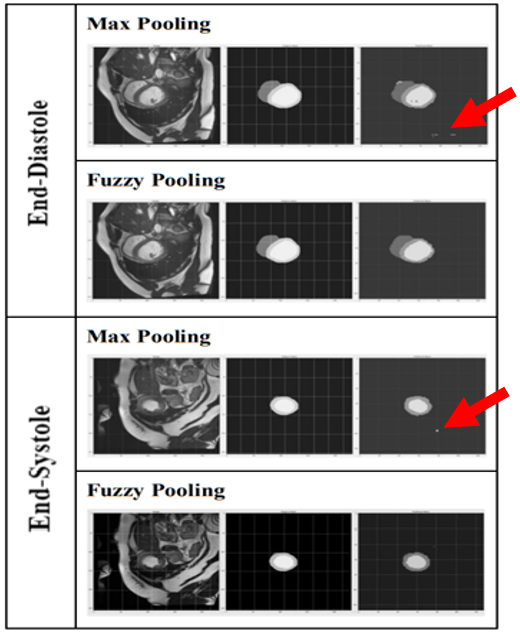
\includegraphics[width=0.86\textwidth]{bab4/ch4-qualitative.png}
	\caption{Qualitative comparison of cardiac structure segmentation obtained using conventional max pooling and the proposed fuzzy pooling for representative End-Diastole and End-Systole images \citep{Riandini2023MeMeA}}
	\label{fig:ch4-qualitative}
\end{figure}

As illustrated in Figure~\ref{fig:ch4-qualitative}, both models successfully identify the major cardiac structures, including the left ventricle (LV), right ventricle (RV), and myocardium (MYO). However, the segmentation produced by the proposed framework exhibits boundaries that more closely follow the expert annotations, indicating improved preservation of anatomical structures during feature extraction and reconstruction. Hence, the structures are observed as: 
%\paragraph{Main observations.}
\begin{itemize}
	\item \textbf{LV:} smoother endocardial contour with fewer boundary irregularities.
	\item \textbf{RV:} improved contour continuity despite its irregular crescent-shaped geometry.
	\item \textbf{MYO:} more uniform myocardial thickness with better preservation of thin anatomical structures.
\end{itemize}

In general, fewer isolated segmentation artifacts and improved anatomical consistency.

The qualitative observations are consistent with the quantitative results presented in Section~\ref{subsec:ch4-quantitative}. The smoother ventricular contours and improved myocardial continuity observed in Figure~\ref{fig:ch4-qualitative} explain the higher Intersection over Union values and lower Hausdorff Distances achieved by the proposed framework. In particular, the substantial reduction in Hausdorff Distance is visually reflected by the improved alignment between the predicted and reference boundaries, whereas the increased IoU corresponds to better overlap of the segmented anatomical regions.

Overall, the qualitative analysis confirms that the proposed framework improves not only numerical segmentation performance but also the anatomical fidelity of the generated segmentation masks. The agreement between the quantitative and qualitative evaluations indicates that integrating fuzzy pooling into the U-Net architecture enhances feature preservation during encoder down-sampling, resulting in more accurate and anatomically consistent cardiac structure segmentation.

\subsection{Overall Discussion}
\label{subsec:ch4-discussion}

The experimental results consistently demonstrate that integrating fuzzy pooling into the encoder of the U-Net architecture improves cardiac structure segmentation without modifying the overall network topology. The improvements observed in both quantitative and qualitative evaluations indicate that preserving richer contextual information during feature aggregation enhances anatomical consistency while reducing boundary errors.

The resulting anatomical myocardium representation established in this chapter provides the structural basis for the subsequent investigations presented in this dissertation. Building upon this framework, Chapter V investigates the influence of different loss functions on myocardium segmentation, whereas Chapter VI extends the analysis toward myocardial scar segmentation and quantitative scar area estimation.

\section{Chapter Summary}
\label{sec:ch4-summary}

This chapter presented an enhanced U-Net framework for cardiac structure segmentation by integrating fuzzy pooling into the encoder pathway. Experimental results demonstrated that the proposed framework improved cardiac structure segmentation compared with the conventional U-Net, providing accurate segmentation of the left ventricle, right ventricle, and myocardium.

The findings demonstrate that preserving richer anatomical information during feature extraction contributes to more accurate cardiac structure segmentation. The resulting anatomical myocardium representation supports the subsequent investigation of loss functions presented in Chapter V and the myocardial scar assessment framework developed in Chapter VI.

		%\cleardoublepage
		\clearpage
		
		\chapter{LOSS FUNCTION INVESTIGATION FOR MYOCARDIUM SEGMENTATION} 
 
\section{Overview}
\label{sec:ch5-intro-overview}  


This chapter presents the second stage of the proposed deep learning framework for myocardial infarction assessment by investigating the influence of different loss functions on myocardium segmentation performance. Building upon the cardiac structure segmentation framework established in Chapter IV, this study aims to identify a loss function that produces a more accurate and reliable anatomical myocardium representation for subsequent myocardial scar segmentation and quantitative scar assessment.  

The previous chapter established an enhanced U-Net framework incorporating fuzzy pooling for cardiac structure segmentation, demonstrating its capability to accurately segment the left ventricle (LV), right ventricle (RV), and myocardium (MYO). The enhanced segmentation backbone adopted in this chapter follows the architecture previously developed in the first stage of this research while maintaining identical preprocessing procedures and training configurations. Although satisfactory segmentation performance was achieved, network architecture alone does not completely determine segmentation quality. During model training, the loss function defines how prediction errors are quantified and guides parameter updates throughout the learning process. Consequently, different loss functions may produce substantially different segmentation characteristics even when an identical network architecture is applied \citep{Ronneberger2015,Jadon2020,Ma2021}. Furthermore, previous work demonstrated that incorporating fuzzy pooling improves feature preservation during down-sampling, providing a suitable segmentation backbone for investigating different optimization objectives \citep{Riandini2023MeMeA}. 

Among the three cardiac structures investigated in Chapter IV, the myocardium represents the most challenging segmentation target. Unlike the relatively homogeneous regions of the left and right ventricles, the myocardium forms a thin ring-shaped anatomical structure with complex boundaries and occupies only a small proportion of the entire cardiac MR image. These characteristics create a pronounced imbalance between foreground and background pixels while simultaneously increasing the difficulty of preserving continuous myocardial contours. As a result, segmentation models trained using conventional pixel-wise loss functions may achieve satisfactory global overlap measurements while still producing suboptimal segmentation of myocardial boundaries, thereby affecting the reliability of subsequent quantitative cardiac analysis and pathology assessment \citep{Milletari2016,Lin2017,Berman2018,Karimi2019,Ma2021}.

Motivated by these challenges, this chapter investigates how different loss functions influence myocardium segmentation performance while maintaining an identical segmentation framework. Five representative loss functions are systematically evaluated, comprising four established loss functions, namely Cross-Entropy, Dice Loss, Focal Loss, and Lovász-Softmax, together with the proposed CrossLov loss. The enhanced U-Net architecture with fuzzy pooling developed in Chapter IV is retained without modification throughout all experiments. Consequently, the experimental design isolates the influence of individual loss functions on myocardium segmentation performance from architectural and implementation factors, allowing performance differences to be attributed solely to the learning characteristics of each investigated loss function \citep{Riandini2025Array}. 

The comparative investigation is conducted from complementary perspectives to provide a comprehensive understanding of the characteristics of each investigated loss function. During the training process, convergence behaviour is analysed through the evolution of training loss, Dice score, computational time, and the best-performing epoch. The resulting segmentation performance is subsequently evaluated quantitatively using the Dice Similarity Coefficient (DSC), Intersection over Union (IoU), and Hausdorff Distance (HD), followed by qualitative visual assessment of myocardial boundary preservation. This integrated evaluation provides complementary information regarding segmentation performance by combining overlap-based measurements, distance-based evaluation, and qualitative visual assessment \citep{Taha2015,Jadon2020,Riandini2025Array}.  

The comparative investigation is conducted from complementary perspectives to provide a comprehensive understanding of the characteristics of each investigated loss function. During the training process, convergence behaviour is analysed through the evolution of training loss, Dice Score, computational time, and the best-performing epoch. The resulting segmentation performance is subsequently evaluated quantitatively using the Dice Similarity Coefficient (DSC), Intersection over Union (IoU), and Hausdorff Distance (HD), followed by qualitative visual assessment of myocardial boundary preservation. This integrated evaluation combines optimization behaviour, overlap-based measurements, distance-based evaluation, and qualitative visual assessment to provide complementary evidence regarding the effectiveness of each investigated loss function \citep{Taha2015,Jadon2020,Ma2021,Riandini2025Array}.

Unlike many segmentation studies that simultaneously modify both the network architecture and the optimization strategy, this study intentionally fixes the segmentation backbone while varying only the loss function. Such a controlled experimental design enables a fair comparison in which differences in segmentation performance can be directly attributed to the optimization objective rather than architectural complexity. Consequently, the findings provide a comprehensive understanding of the complementary strengths and limitations of pixel-wise, region-based, and hybrid learning objectives for myocardium segmentation under an identical segmentation framework \citep{Riandini2025Array}.

The primary contribution of this chapter is to identify an effective loss function for reliable myocardium segmentation using a fixed enhanced U-Net framework with fuzzy pooling. Rather than introducing a new segmentation architecture, this study provides a comprehensive understanding of how different learning objectives influence myocardium segmentation performance and identifies the most suitable loss function for accurate and reliable myocardium segmentation under a fixed segmentation method. The findings presented in this chapter establish a more reliable myocardium representation that supports the residual attention-based myocardial scar assessment framework presented in Chapter VI. 

\section{Myocardium Segmentation Framework}
\label{sec:ch5-framework} 

\subsection{Framework Overview}
\label{subsec:ch5-overview}  

Building upon the enhanced U-Net framework with fuzzy pooling established in Chapter IV, this chapter investigates the influence of different loss functions on myocardium segmentation while maintaining an identical segmentation architecture. Rather than proposing a new segmentation network, the enhanced U-Net with fuzzy pooling developed in the previous chapter is retained as a fixed segmentation backbone throughout this study. Consequently, the selected loss function becomes the sole independent experimental variable, enabling the influence of different optimization objectives on myocardium segmentation performance to be investigated without interference from architectural modifications, preprocessing procedures, or training configurations.   

Unlike Chapter IV, which addressed the simultaneous segmentation of the left ventricle (LV), right ventricle (RV), and myocardium (MYO), the present study focuses exclusively on myocardium ring segmentation. This narrower scope is motivated by the anatomical characteristics of the myocardium, which forms a thin ring-shaped structure with complex geometry, indistinct boundaries, and relatively small spatial occupancy within cardiac MR images. These characteristics create a pronounced foreground-background class imbalance while simultaneously increasing the difficulty of preserving continuous myocardial contours. Consequently, myocardium segmentation requires learning objectives capable of improving both regional overlap and boundary consistency to achieve anatomically reliable segmentation results \citep{Milletari2016,Berman2018,Karimi2019,Ma2021}

The overall experimental workflow adopted in this chapter is illustrated in Figure~\ref{fig:ch5-framework}. The workflow begins with cine cardiac MR images acquired from the ACDC dataset, followed by image preprocessing before being provided as input to the enhanced U-Net incorporating fuzzy pooling. During network training, five representative loss functions, namely Cross-Entropy, Dice Loss, Focal Loss, Lovász-Softmax, and the proposed CrossLov loss, are independently incorporated into the optimization process. Throughout all experiments, the network architecture, dataset partition, optimizer, hyperparameter settings, and evaluation protocol are maintained without modification, ensuring that the investigated loss function constitutes the only independent experimental variable. This controlled experimental design enables a fair comparison in which the observed performance differences can be attributed solely to the learning characteristics of each investigated loss function rather than to variations in network architecture or implementation \citep{Riandini2025Array}. 

Following model training, the resulting myocardium segmentation masks are evaluated through complementary quantitative and qualitative analyses. Training behaviour is first examined using convergence characteristics, training loss, Dice Score, computational time, and the best-performing epoch achieved by each investigated loss function. The segmentation results are subsequently evaluated using the Dice Similarity Coefficient (DSC), Intersection over Union (IoU), and Hausdorff Distance (HD), followed by qualitative visual comparison of representative myocardium segmentation results. Collectively, these complementary evaluations provide a comprehensive understanding of how different optimization objectives influence myocardium segmentation performance and facilitate the identification of the most appropriate loss function for accurate and reliable myocardium segmentation under a fixed segmentation framework \citep{Taha2015,Jadon2020,Ma2021,Riandini2025Array}.

\begin{figure}[htbp]
	\centering
	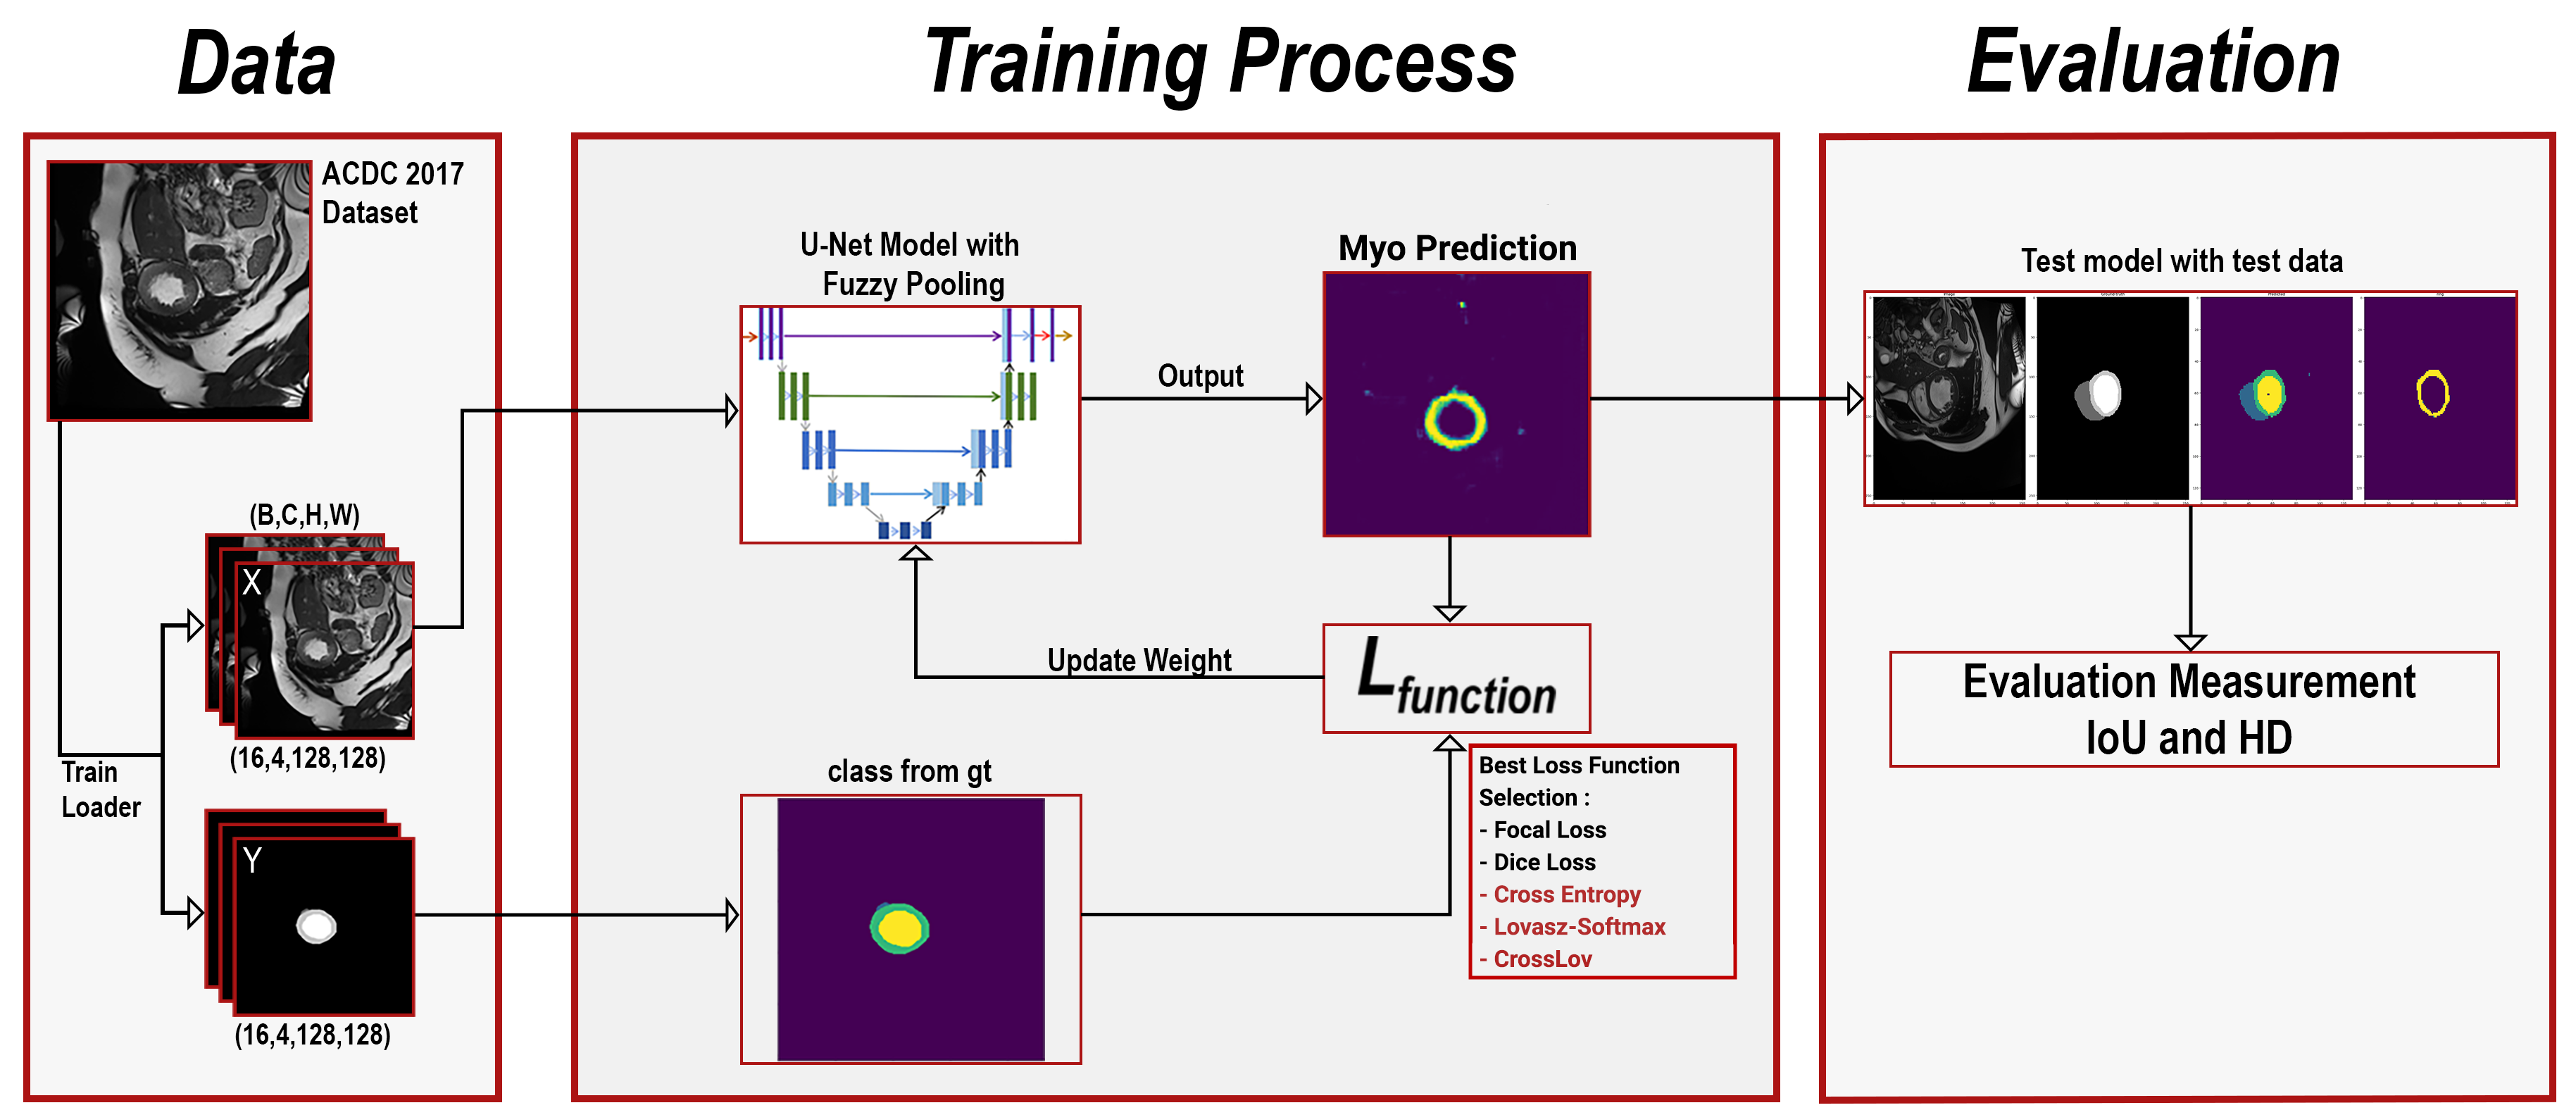
\includegraphics[width=0.86\textwidth]{bab5/ch5-framework.png}
	\caption{Overall framework for myocardium segmentation using the enhanced U-Net with fuzzy pooling and the investigated loss functions \citep{Riandini2025Array}}
	\label{fig:ch5-framework}
\end{figure}

\subsection{Fixed Enhanced U-Net with Fuzzy Pooling}
\label{subsec:ch5-fixedUnet}

The segmentation network employed throughout this chapter is identical to the enhanced U-Net with fuzzy pooling established and experimentally validated in Chapter IV. Accordingly, no architectural modifications are introduced in the present study. Instead, the previously developed segmentation network is retained as a fixed backbone to ensure that the investigated loss function remains the only independent variable affecting myocardium segmentation performance. By maintaining an identical network architecture throughout all experiments, the influence of architectural design is eliminated, enabling a fair and controlled comparison of different optimization objectives. 

The adopted network preserves the encoder-decoder architecture of the conventional U-Net while incorporating fuzzy pooling within the encoder during the down-sampling process, as illustrated in Figure~\ref{fig:ch5-architecture}. Unlike conventional max-pooling, fuzzy pooling performs feature aggregation based on fuzzy membership values, allowing representative features to be preserved while reducing the loss of spatial information during feature extraction. Combined with skip connections between the encoder and decoder, this strategy facilitates the reconstruction of anatomically consistent myocardium segmentation masks while preserving fine structural details. The effectiveness of this architecture for cardiac MR image segmentation has been demonstrated in Chapter IV and therefore serves as the fixed segmentation backbone throughout the present investigation. 

Since the primary objective of this chapter is to investigate the influence of different loss functions rather than to develop a new segmentation architecture, all architectural components are maintained without modification throughout the study. These components include the enhanced U-Net architecture, fuzzy pooling mechanism, image preprocessing procedure, optimizer, hyperparameter configuration, and dataset partition. Consequently, any observed differences in segmentation performance can be attributed exclusively to the learning behaviour of the investigated loss functions rather than to variations in network architecture or experimental settings \citep{Riandini2025Array}. 

The fuzzy pooling mechanism incorporated into the enhanced U-Net has been comprehensively described and experimentally validated in Chapter IV. Therefore, its mathematical formulation and operational procedure are not repeated in this chapter. Instead, the present investigation concentrates on how different optimization objectives influence the learning behaviour of the same segmentation network and subsequently affect myocardium segmentation performance under identical experimental conditions. 

\begin{figure}[htbp]
	\centering
	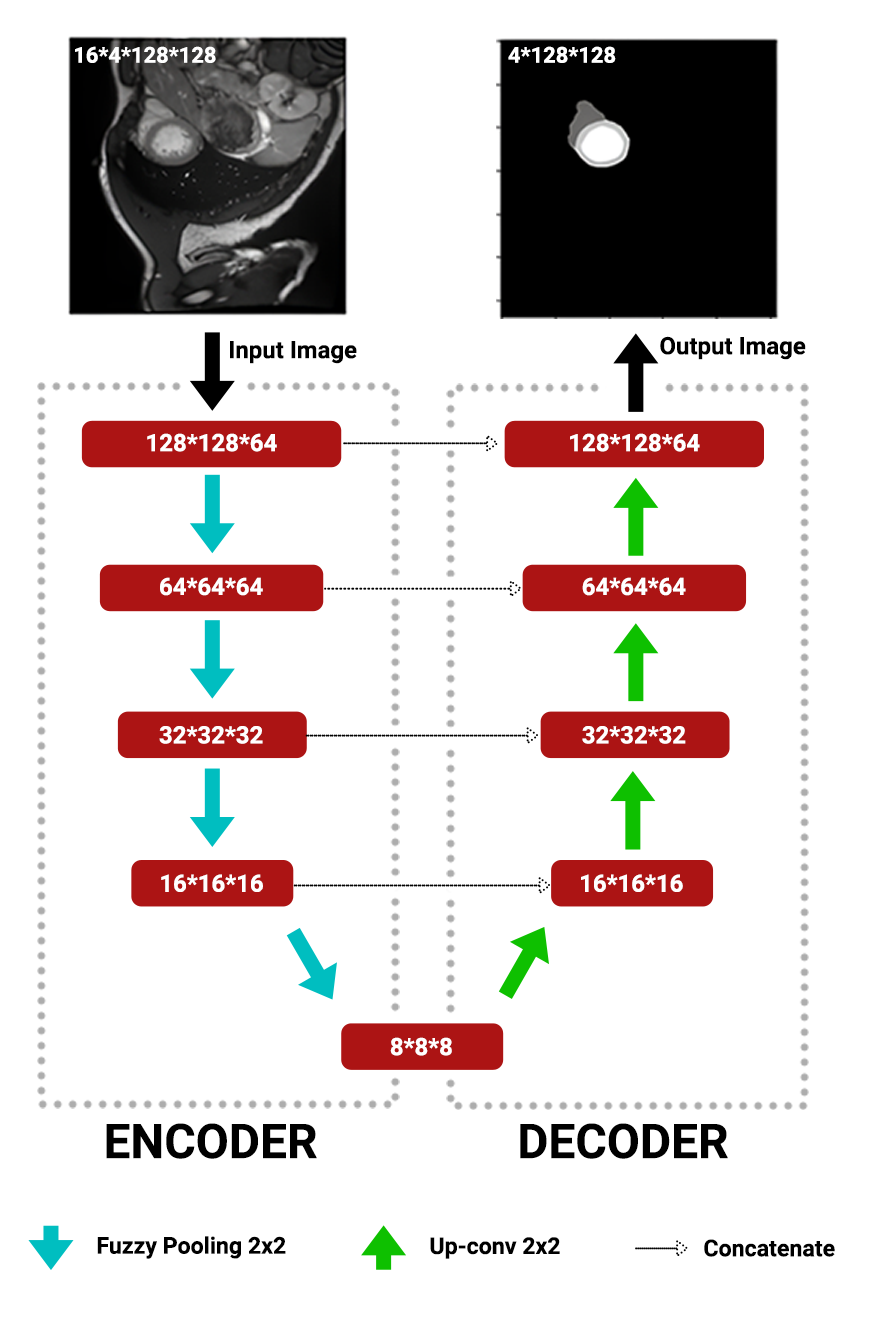
\includegraphics[width=0.86\textwidth]{bab5/ch5-architecture.png}
	\caption{Enhanced U-Net architecture applying fuzzy pooling for myocardium segmentation \citep{Riandini2025Array}}
	\label{fig:ch5-architecture}
\end{figure}

\subsection{Loss Function Investigation Strategy }
\label{subsec:ch5-LossInvestigation}

The primary objective of this chapter is to systematically investigate how different optimization objectives influence myocardium segmentation performance under an identical segmentation framework. To achieve this objective, five representative loss functions were selected based on their complementary learning characteristics, encompassing pixel-wise classification, region-overlap optimization, and hybrid learning strategies. By investigating loss functions with different optimization principles, this study aims to provide a comprehensive understanding of how the learning objective affects myocardium segmentation performance while maintaining identical network architecture and experimental settings \citep{Jadon2020,Ma2021}. 

Accordingly, five loss functions were investigated, comprising four established loss functions, namely Cross-Entropy, Dice Loss, Focal Loss, and Lovász-Softmax, together with the proposed CrossLov loss, which combines Cross-Entropy and Lovász-Softmax within a unified optimization objective. Cross-Entropy represents the conventional pixel-wise learning strategy, Dice Loss directly optimizes region overlap, Focal Loss emphasizes difficult-to-classify pixels under class imbalance, whereas Lovász-Softmax provides direct optimization of the Intersection over Union (IoU). The proposed CrossLov loss integrates pixel-wise classification with region-based optimization to exploit the complementary advantages of both learning paradigms \citep{Lin2017,Berman2018,Ma2021,Riandini2025Array}.

Based on their underlying optimization principles, the investigated loss functions can be grouped into three categories, as summarized in Table~\ref{tab:ch5-loss-classification}.

\begin{table}[htbp]
	\centering
	\caption{Classification of investigated loss functions}
	\label{tab:ch5-loss-classification}
	
	\small
	\renewcommand{\arraystretch}{1.3}
	\begin{tabular}{l l l}
		\toprule
		\textbf{Category} & \textbf{Loss Function} & \textbf{Learning Characteristic} \\
		\midrule
		Pixel-wise & Cross-Entropy & Pixel classification \\
		Pixel-wise & Focal Loss & Hard-sample emphasis \\
		Region-based & Dice Loss & Region overlap \\
		Region-based & Lov\'asz-Softmax & IoU-oriented learning \\
		Hybrid & CrossLov & Pixel-wise and region-based learning \\
		\bottomrule
		\multicolumn{3}{@{}l}{\vspace{4pt}\footnotesize \textit{Source:} Adapted from \citet{Riandini2025Array}.}
	\end{tabular}
\end{table}

As presented in Table~\ref{tab:ch5-loss-classification}, the investigated loss functions represent complementary optimization strategies. Pixel-wise loss functions focus primarily on individual pixel classification, region-based loss functions directly optimize segmentation overlap, whereas the proposed hybrid loss combines both optimization characteristics within a unified learning objective. This categorization facilitates a systematic comparison of their respective learning behaviours under identical experimental conditions while providing a conceptual basis for interpreting the quantitative and qualitative results presented in the subsequent sections. 

To ensure a fair comparative investigation, all experiments were conducted using an identical segmentation framework, including the enhanced U-Net architecture with fuzzy pooling, dataset partition, image preprocessing procedure, optimizer, hyperparameter configuration, and evaluation protocol. Consequently, the investigated loss function remained the only independent experimental variable throughout the study. The comparative analysis subsequently evaluates each loss function using training behaviour, Dice Similarity Coefficient (DSC), Intersection over Union (IoU), Hausdorff Distance (HD), and qualitative visual assessment. Collectively, these complementary evaluation criteria provide comprehensive evidence regarding the effectiveness of each investigated optimization objective for myocardium segmentation under a fixed segmentation framework \citep{Taha2015,Riandini2025Array}.

\subsection{Training Strategy }
\label{subsec:ch5-Training-Strategy}

To ensure a fair and reproducible comparative investigation, all investigated loss functions were trained under an identical training strategy. Since the objective of this chapter is to evaluate the influence of different optimization objectives on myocardium segmentation performance, every component of the segmentation framework established in Chapter IV was maintained without modification throughout all experiments. Consequently, the enhanced U-Net architecture with fuzzy pooling, dataset partition, image preprocessing procedure, optimizer, hyperparameter configuration, and evaluation protocol remained identical for every experiment. Under these controlled conditions, the investigated loss function constituted the only independent experimental variable, enabling differences in segmentation performance to be directly attributed to the learning characteristics of each optimization objective. 

The standardized training strategy adopted throughout this comparative investigation is summarized in Table~\ref{tab:ch5-training-strategy}. Each investigated loss function was independently incorporated into the training process while preserving an identical segmentation framework and experimental configuration. Maintaining consistent training conditions minimizes potential experimental bias and ensures that the observed performance differences originate exclusively from the investigated loss functions rather than from variations in network architecture or implementation settings.

\begin{table}[htbp]
	\centering
	\caption{Standardized training strategy adopted in this study}
	\label{tab:ch5-training-strategy}
	
	\small
	\renewcommand{\arraystretch}{1.3}
	\begin{tabularx}{\textwidth}{
			>{\raggedright\arraybackslash}p{0.28\textwidth}
			>{\raggedright\arraybackslash}X
		}
		\toprule
		\textbf{Training Stage} & \textbf{Purpose} \\
		\midrule
		Network initialization & Initialize the enhanced U-Net with fuzzy pooling using identical architecture and hyperparameter settings. \\ \addlinespace
		Model optimization & Train the network using one investigated loss function while maintaining identical dataset, preprocessing procedure, optimizer, learning rate, batch size, and training epochs. \\ \addlinespace
		Training monitoring & Monitor training loss, Dice Score, computational time, and the best-performing epoch throughout the training process. \\ \addlinespace
		Performance evaluation & Evaluate segmentation performance using the Dice Similarity Coefficient (DSC), Intersection over Union (IoU), Hausdorff Distance (HD), and qualitative visual assessment. \\
		\bottomrule
		\multicolumn{2}{@{}l}{\vspace{4pt}\footnotesize \textit{Source:} Adapted from \citet{Riandini2025Array}.}
	\end{tabularx}
\end{table}

Following the training process, the resulting segmentation models were evaluated using an identical assessment protocol to ensure objective comparison among the investigated loss functions. Quantitative performance was assessed using the Dice Similarity Coefficient (DSC), Intersection over Union (IoU), and Hausdorff Distance (HD), whereas qualitative evaluation was conducted through visual comparison between the predicted myocardium segmentation masks and the corresponding ground-truth annotations. In addition, the convergence behaviour of each investigated loss function was analysed by examining training loss, Dice Score, computational time, and the best-performing epoch achieved during optimization. These complementary evaluations provide a comprehensive assessment of optimization behaviour, segmentation accuracy, boundary localization, and anatomical consistency under identical experimental conditions \citep{Taha2015,Riandini2025Array}. 

By adopting a standardized training strategy throughout all comparative experiments, this study establishes a controlled experimental environment in which the influence of the investigated loss functions can be evaluated objectively and reproducibly. The training behaviour and segmentation performance obtained from this protocol are subsequently analysed in the following sections to determine the most suitable optimization objective for accurate and reliable myocardium segmentation using the enhanced U-Net framework with fuzzy pooling. 

\section{Materials and Experimental Setup}
\label{sec:ch5-Experiment-Setup}

This section describes the materials and experimental setup adopted to investigate the influence of different loss functions on myocardium segmentation performance. To ensure a fair and reproducible comparative investigation, all experiments were conducted using the same dataset, segmentation architecture, preprocessing procedure, training configuration, and evaluation protocol established in Chapter IV. Consequently, the investigated loss function remained the only independent experimental variable throughout the study, enabling differences in segmentation performance to be attributed solely to the learning characteristics of each optimization objective. The standardized experimental setup presented in this section provides the basis for interpreting the comparative results reported in the subsequent sections. 

\subsection{Dataset}
\label{subsec:ch5-Dataset}

The experimental evaluation was conducted using the Automated Cardiac Diagnosis Challenge (ACDC) 2017 dataset, which contains manually annotated cine cardiac magnetic resonance (CMR) images of the left ventricle (LV), right ventricle (RV), and myocardium (MYO). Consistent with the experimental protocol established in Chapter IV, the present study exclusively utilizes the myocardium annotations to investigate the influence of different optimization objectives on myocardium ring segmentation. By restricting the investigation to a single anatomical structure while maintaining an identical segmentation framework, the effect of the investigated loss functions can be evaluated under controlled experimental conditions. 

To maintain experimental consistency, the same dataset partition adopted in Chapter IV was retained throughout the investigation. The distribution of the training and testing images is summarized in Table~\ref{tab:ch5-dataset-distribution}.

\begin{table}[htbp]
	\centering
	\caption{Dataset distribution}
	\label{tab:dataset_distribution}
	
	\small
	\setlength{\heavyrulewidth}{\lightrulewidth}
	\renewcommand{\arraystretch}{1.3}
	\begin{tabular}{lcc}
		\toprule
		\textbf{Dataset} & \textbf{Number of Images} & \textbf{Percentage} \\
		\midrule
		Training & 1,902 & 85\% \\
		Testing & 286 & 15\% \\ \midrule
		\textbf{Total} & \textbf{2,188} & \textbf{100\%} \\ \bottomrule
		\multicolumn{3}{@{}l}{\vspace{4pt}\footnotesize \textit{Source:} Adapted from \citet{Riandini2026Access}.}
	\end{tabular}
\end{table}

All preprocessing procedures, including image normalization, resizing, and annotation preparation, were performed identically for every investigated loss function. Maintaining an identical preprocessing pipeline ensures that variations in segmentation performance originate exclusively from differences in the adopted optimization objective rather than from inconsistencies in data preparation. 

\subsection{Experimental Environment}
\label{subsec:ch5-experiment-enviroment}

All comparative experiments were conducted using an identical computational environment to ensure consistency during model training and performance evaluation. The hardware and implementation settings employed throughout the investigation are summarized in Table~\ref{tab:ch5-experiment-environment}.

\begin{table}[htbp]
	\centering
	\caption{Experimental Environment}
	\label{tab:experimental_environment}
	
	\small
	\setlength{\heavyrulewidth}{\lightrulewidth}
	\renewcommand{\arraystretch}{1.3}
	
	% \resizebox DIHAPUS agar tabel tidak ditarik melar
	\begin{tabular}{ll}
		\toprule
		\textbf{Component} & \textbf{Specification} \\ \midrule
		GPU                 & Tesla T4 \\
		GPU Memory          & 32 GB \\
		Training Epochs     & 100 \\
		Input Tensor Format & $16 \times 4 \times 128 \times 128$ \\ \bottomrule
	\end{tabular}
\end{table}

The computational environment presented in Table~\ref{tab:ch5-experiment-environment} was maintained without modification for all comparative experiments. Consequently, the computational performance and segmentation accuracy obtained by each investigated loss function were evaluated under identical hardware conditions, thereby ensuring a fair comparison of the resulting optimization behaviour. 

\subsection{Training Configuration}
\label{subsec:ch5-training-config}

To ensure a fair comparative investigation, every investigated loss function was trained using an identical network configuration. Apart from the optimization objective, all components of the segmentation framework, including the enhanced U-Net architecture, fuzzy pooling mechanism, preprocessing procedure, optimizer, dataset partition, and hyperparameter configuration, were maintained without modification throughout the study. The adopted training configuration is summarized in Table~\ref{tab:ch5-training-config}.

\begin{table}[htbp]
	\centering
	\caption{Training configuration adopted in this study}
	\label{tab:ch5-training-config}
	
	\small
	\setlength{\heavyrulewidth}{\lightrulewidth}
	\renewcommand{\arraystretch}{1.3}
	\begin{tabularx}{\textwidth}{
			>{\raggedright\arraybackslash}p{0.32\textwidth}
			>{\raggedright\arraybackslash}X
		}
		\toprule
		\textbf{Parameter} & \textbf{Configuration} \\
		\midrule
		Segmentation Network & Enhanced U-Net \\
		Pooling Method & Fuzzy Pooling \\
		Target Structure & Myocardium (MYO) \\
		Input Image Size & 128 $\times$ 128 pixels \\
		Number of Classes & 4 \\
		Batch Size & 16 \\
		Investigated Loss Functions & Cross-Entropy, Dice Loss, Focal Loss, Lov\'asz-Softmax, CrossLov \\
		Training Epochs & 100 \\
		\bottomrule
		\multicolumn{2}{@{}l}{\vspace{4pt}\footnotesize \textit{Source:} Adapted from \citet{Riandini2025Array}.}
	\end{tabularx}
\end{table}

The standardized configuration summarized in Table~\ref{tab:ch5-training-config} ensures that the investigated loss function remains the only experimental factor differing among all training sessions. Therefore, any observed differences in segmentation performance can be interpreted as the consequence of the adopted optimization objective rather than differences in network architecture or training settings. 

\subsection{Evaluation Metrics}
\label{subsec:ch5-eval-metric}

The effectiveness of each investigated loss function was evaluated using quantitative metrics that are widely employed in medical image segmentation studies. To provide complementary assessments of segmentation performance, overlap-based and boundary-based metrics were jointly adopted. The evaluation metrics used throughout this study are summarized in Table~\ref{tab:ch5-eval-metric}.

\begin{table}[htbp]
	\centering
	\caption{Evaluation metrics used in this study}
	\label{tab:ch5-eval-metric}
	
	\small
	\setlength{\heavyrulewidth}{\lightrulewidth}
	\renewcommand{\arraystretch}{1.3}
	\begin{tabularx}{\textwidth}{
			>{\raggedright\arraybackslash}p{0.32\textwidth}
			>{\raggedright\arraybackslash}X
		}
		\toprule
		\textbf{Metric} & \textbf{Purpose} \\
		\midrule
		Dice Similarity Coefficient (DSC) & Measures the overlap between the predicted segmentation and the ground-truth annotation. \\ \addlinespace
		Intersection over Union (IoU) & Evaluates regional agreement between the predicted myocardium segmentation and the reference annotation. \\ \addlinespace
		Hausdorff Distance (HD) & Measures the maximum boundary distance between the predicted segmentation and the reference annotation. \\
		\bottomrule
		\multicolumn{2}{@{}l}{\vspace{4pt}\footnotesize \textit{Source:} Adapted from \citet{Taha2015}.}
	\end{tabularx}
\end{table}

In addition to quantitative evaluation, qualitative visual assessment was performed by comparing the predicted myocardium segmentation masks with the corresponding ground-truth annotations. The combination of quantitative measurements and visual inspection provides a more comprehensive understanding of segmentation performance, particularly for assessing boundary continuity and anatomical consistency. The comparative results obtained using these evaluation criteria are presented and discussed in the following section. 

\section{Experimental Results and Discussion}
\label{sec:ch5-experiment-result-discuss}

This section presents a comparative analysis of the investigated loss functions using identical experimental conditions. The discussion is organized according to the experimental evidence obtained from the training process, quantitative evaluation, and qualitative visual assessment. By maintaining the same segmentation framework throughout the investigation, the observed performance differences can be attributed solely to the investigated loss functions.

\subsection{Training Behaviour Analysis}
\label{subsec:ch5-training-analysis}

Before comparing the final segmentation performance achieved by the investigated loss functions, it is essential to first analyse their behaviour during the network training process. Although all comparative experiments were conducted using the same enhanced U-Net architecture, fuzzy pooling strategy, dataset partition, preprocessing procedure, optimizer, hyperparameter configuration, and training protocol, the optimization behaviour varies according to the selected loss function. Consequently, analysing the training process provides valuable insight into convergence stability, learning efficiency, computational cost, and segmentation capability before evaluating the final quantitative and qualitative segmentation results.
The training behaviour of the five investigated loss functions is presented in Figure~\ref{fig:ch5-training-performance}, which summarizes the evolution of the training loss, testing loss, Dice score, computational time, and the best-performing training epoch obtained under identical experimental conditions.

\begin{figure}[htbp]
	\centering
	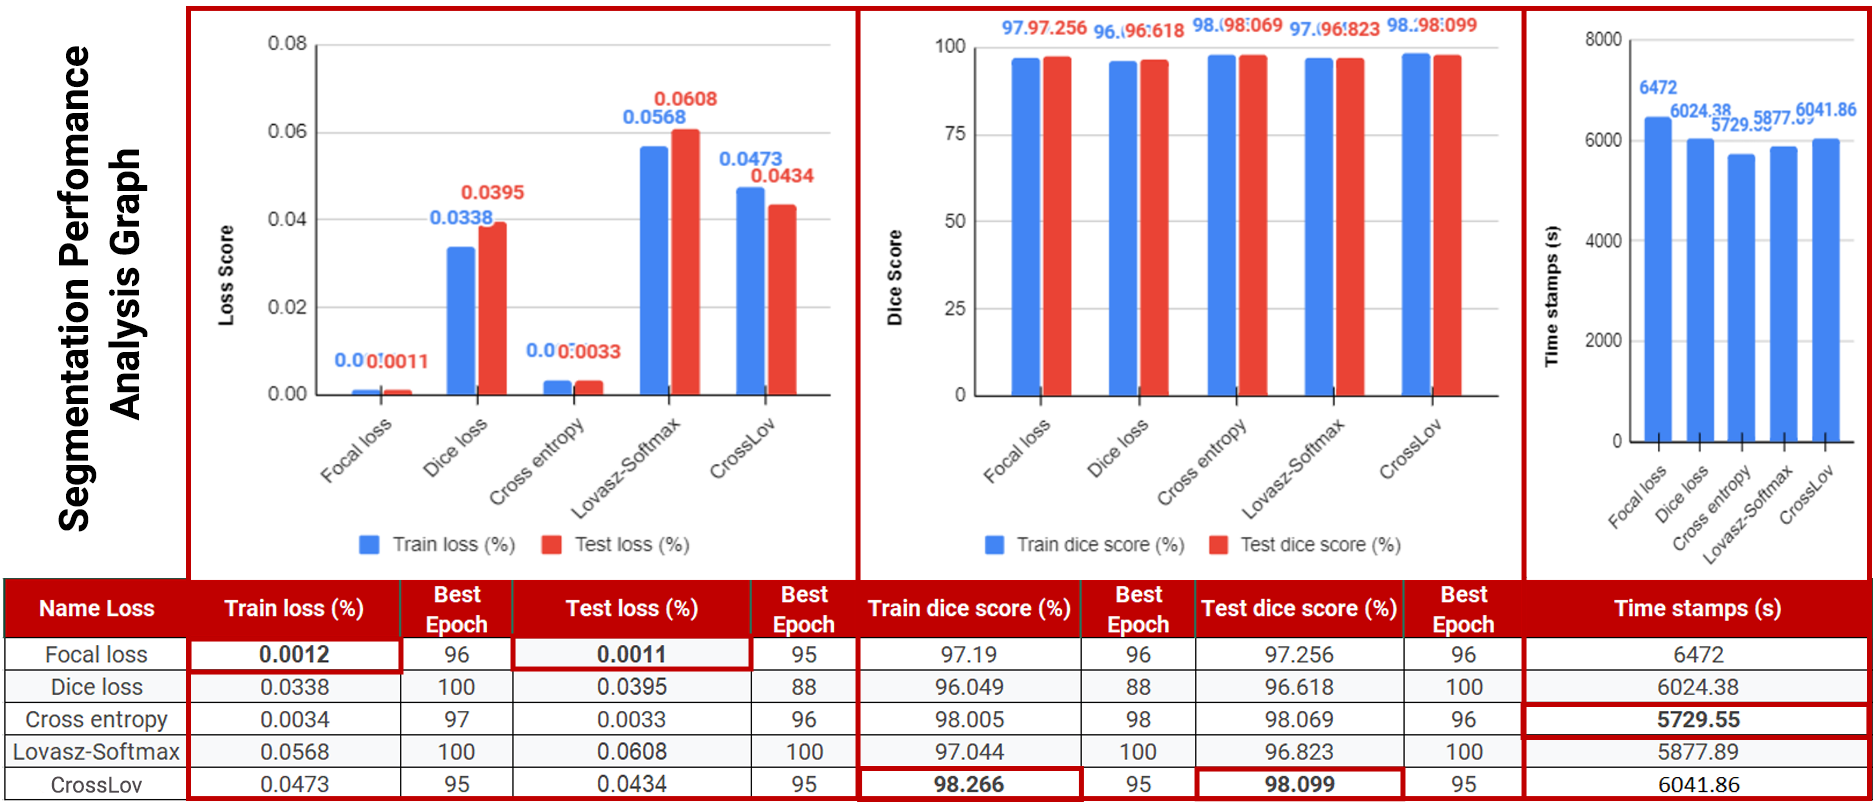
\includegraphics[width=\textwidth]{bab5/ch5-training-performance.png}
	\caption{Training performance of the investigated loss functions showing the training loss, testing loss, Dice score, computational time, and best-performing epoch obtained for each evaluated loss function \protect\citep{Riandini2025Array}}
	\label{fig:ch5-training-performance}
\end{figure}

As illustrated in Figure~\ref{fig:ch5-training-performance}, the investigated loss functions demonstrate noticeably different optimization behaviours despite being trained using an identical segmentation framework. The training and testing loss curves indicate that Focal Loss consistently achieved the smallest objective function values throughout the optimization process, suggesting that it was highly effective in minimizing prediction error during learning. However, the reduction of the optimization objective did not necessarily correspond to the highest segmentation accuracy, indicating that convergence of the loss function alone is insufficient to evaluate segmentation performance comprehensively.

A different trend is observed from the Dice score analysis. While Focal Loss produced the lowest optimization loss, CrossLov consistently achieved the highest Dice score for both the training and testing datasets. This observation suggests that combining Cross-Entropy and Lovász-Softmax enables the optimization process to simultaneously preserve pixel-wise classification accuracy and region-level overlap. Consequently, CrossLov generated more accurate myocardium segmentation even though its optimization loss was not the smallest among the investigated methods.

Figure~\ref{fig:ch5-training-performance} also reveals differences in computational efficiency. Among the investigated loss functions, Cross-Entropy required the shortest training time to complete the full optimization process, whereas Focal Loss required the longest computational time under the same hardware configuration. Although the computational difference is relatively modest, this observation indicates that optimization objectives emphasizing difficult samples may require additional computational resources during training.

To facilitate interpretation of the training behaviour illustrated in Figure~\ref{fig:ch5-training-performance}, the principal observations are summarized in  Table~\ref{tab:ch5-summary-training-behaviour}.

\begin{table}[htbp]
	\centering
	\caption{Summary of Training Behaviour based on Figure~\ref{fig:ch5-training-performance}}
	\label{tab:ch5-summary-training-behaviour}
	
	\small
	\setlength{\heavyrulewidth}{\lightrulewidth}
	\renewcommand{\arraystretch}{1.3}
	
	% \resizebox DIHAPUS agar font kembali ke ukuran normal/proporsional
	\begin{tabular}{ll}
		\toprule
		\textbf{Observation} & \textbf{Result} \\ \midrule
		Lowest Training Loss       & Focal Loss (0.0012, Epoch 96) \\
		Lowest Testing Loss        & Focal Loss (0.0011, Epoch 95) \\
		Highest Training Dice Score & CrossLov (98.266\%, Epoch 95) \\
		Highest Testing Dice Score  & CrossLov (98.099\%, Epoch 95) \\
		Shortest Training Time     & Cross-Entropy (5729.55 s) \\
		Longest Training Time      & Focal Loss (6472 s) \\ \bottomrule
	\end{tabular}
\end{table}

The observations summarized in Table~\ref{tab:ch5-summary-training-behaviour} confirm that each investigated loss function exhibits distinct optimization characteristics despite sharing an identical segmentation framework. Focal Loss demonstrated superior convergence behaviour by minimizing the optimization objective more effectively than the remaining methods, whereas Cross-Entropy provided the highest computational efficiency by requiring the shortest training time. In contrast, CrossLov consistently achieved the highest Dice scores on both the training and testing datasets, indicating that balanced optimization of pixel-wise classification and region-level overlap contributes more effectively to segmentation accuracy than minimizing the loss function alone.

These findings demonstrate that convergence behaviour, computational efficiency, and segmentation accuracy represent complementary aspects of optimization performance rather than interchangeable evaluation criteria. A loss function producing the smallest optimization error does not necessarily generate the highest-quality segmentation results, while rapid convergence does not automatically indicate superior anatomical representation. Therefore, comprehensive evaluation using segmentation-oriented performance metrics is required to determine the most appropriate optimization objective for myocardium segmentation.

The influence of each investigated loss function on segmentation accuracy is further analysed quantitatively in the following section using the \textbf{Dice Similarity Coefficient (DSC)}, Intersection \textbf{over Union (IoU)}, and \textbf{Hausdorff Distance (HD)} to provide a comprehensive comparison of overlap accuracy and boundary consistency.

\subsection{Quantitative Comparison of Loss Functions}
\label{subsec:ch5-quantitative-compare-loss}

The quantitative performance of the investigated loss functions was evaluated using the Dice Similarity Coefficient (DSC), Intersection over Union (IoU), and Hausdorff Distance (HD). These complementary metrics provide comprehensive assessment of segmentation performance by simultaneously evaluating regional overlap and boundary agreement between the predicted myocardium segmentation and the corresponding ground-truth annotation. The complete quantitative results obtained under identical experimental conditions are presented in Table~\ref{tab:ch5-quantitative-compare-loss}.

\begin{sidewaystable}[htbp]
	\centering
	\caption{Evaluation results of state-of-the-art models and proposed CrossLov using IoU, HD, and Dice Score}
	\label{tab:ch5-quantitative-compare-loss}
	
	% 1. Ubah font menjadi lebih kecil satu tingkat agar muat di margin
	\footnotesize 
	% 2. Rapatkan jarak antar kolom secara signifikan
	\setlength{\tabcolsep}{3pt} 
	\setlength{\heavyrulewidth}{\lightrulewidth}
	% 3. Kurangi sedikit padding vertikal
	\renewcommand{\arraystretch}{1.15} 
	
	\begin{tabular}{llccccc}
		\toprule
		\textbf{Evaluation metric} & \textbf{Class} & \multicolumn{5}{c}{\textbf{Name loss}} \\ \cmidrule(lr){3-7}
		& & \specialcell{\textbf{Focal Loss} \\ \citep{Lin2017}} & \specialcell{\textbf{Dice Loss} \\ \citep{Wyburd2021,Ma2021}} & \specialcell{\textbf{Cross entropy} \\ \citep{Yeung2022}} & \specialcell{\textbf{Lovasz-Softmax} \\ \citep{Berman2018}} & \textbf{CrossLov} \\
		\midrule
		\multirow{2}{*}{Average IoU (\%)} & MYO + LV + RV & 91.862 & 87.647 & 81.103 & 88.763 & \textbf{93.691} \\
		& MYO & 51.965 & 89.4 & 51.959 & \textbf{90.68} & 60.262 \\ \addlinespace
		\multirow{2}{*}{Highest IoU (\%)} & MYO + LV + RV & \textbf{100} & 95.909 & 94.54 & 97.757 & \textbf{100} \\
		& MYO & \textbf{100} & \textbf{100} & \textbf{100} & \textbf{100} & \textbf{100} \\ \addlinespace
		\multirow{2}{*}{Lowest IoU (\%)} & MYO + LV + RV & 49.972 & 33.274 & 33.3 & 34.955 & \textbf{49.987} \\
		& MYO & 48.3 & \textbf{67.152} & 49.148 & 49.88 & 49.633 \\ \addlinespace
		\multirow{2}{*}{Average HD} & MYO + LV + RV & 2.935 & 3.27 & 4.598 & 3.251 & \textbf{2.816} \\
		& MYO & 1.338 & 1.648 & 1.689 & 1.527 & \textbf{1.309} \\ \addlinespace
		\multirow{2}{*}{Highest HD} & MYO + LV + RV & 4.242 & 6 & 4 & 8.062 & 6.928 \\
		& MYO & 1.746 & 2.922 & \textbf{1.734} & 2.862 & 2.221 \\ \addlinespace
		\multirow{2}{*}{Lowest HD} & MYO + LV + RV & \textbf{1} & \textbf{1} & \textbf{0} & 0.43 & 0.0004 \\
		& MYO & 0.012 & \textbf{3.60E-06} & 7.63E-03 & -- & 97.256 \\ \addlinespace
		Dice score & & 96.823 & 96.618 & 98.069 & 96.823 & \textbf{98.099} \\
		\bottomrule
		\multicolumn{7}{@{}l}{\vspace{4pt}\textit{Source:} Adapted from \citet{Riandini2025Array}.}
	\end{tabular}
\end{sidewaystable}

The quantitative results presented in Table~\ref{tab:ch5-quantitative-compare-loss} demonstrate that the investigated loss functions exhibit different optimization characteristics depending on the evaluation metric considered. Although all experiments employed an identical segmentation framework, variations in the optimization objective resulted in measurable differences in overlap accuracy and boundary consistency. To facilitate interpretation of these findings, the principal quantitative observations are summarized in Table~\ref{tab:ch5-summary-quantitative-performance}.

\begin{table}[htbp]
	\centering
	\caption{Summary of Quantitative Performance based on Table~\ref{tab:ch5-quantitative-compare-loss}}
	\label{tab:ch5-summary-quantitative-performance}
	
	\small
	% Menyamakan ketebalan garis booktabs agar seragam tipis
	\setlength{\heavyrulewidth}{\lightrulewidth}
	% Memberikan padding vertikal yang lega (tidak menjepit judul kolom)
	\renewcommand{\arraystretch}{1.3}
	
	\resizebox{\linewidth}{!}{%
		\begin{tabular}{lll}
			\toprule
			\textbf{Evaluation Criterion} & \textbf{Best Result} & \textbf{Loss Function} \\ \midrule
			Average IoU (MYO + LV + RV)   & 93.691\%             & CrossLov \\
			Average IoU (MYO)             & 90.680\%             & Lov\'asz-Softmax \\
			Lowest Average HD (MYO + LV + RV) & 2.816             & CrossLov \\
			Lowest Average HD (MYO)       & 1.309                & CrossLov \\
			Highest Dice Score            & 98.099\%             & CrossLov \\ \bottomrule
		\end{tabular}%
	}
\end{table}

The summary presented in Table~\ref{tab:ch5-summary-quantitative-performance} indicates that no single loss function consistently achieved the best result for every evaluation criterion. Instead, each investigated optimization objective emphasized different aspects of myocardium segmentation performance. Lovász-Softmax achieved the highest Average IoU for myocardium segmentation, indicating its effectiveness in maximizing regional overlap between the predicted myocardium and the reference annotation. This observation is consistent with the optimization objective of \textbf{Lovász-Softmax}, which directly approximates the IoU metric during network training.

In contrast, \textbf{CrossLov} demonstrated the most balanced overall performance across the evaluated metrics. In addition to achieving the highest Dice Similarity Coefficient, CrossLov also produced the lowest Hausdorff Distance for both the overall cardiac structures and the myocardium. These findings indicate that the combination of Cross-Entropy and Lovász-Softmax enables the network to preserve accurate pixel-wise classification while simultaneously improving regional overlap and boundary localization. Consequently, the resulting segmentation masks exhibit both high overlap accuracy and improved anatomical consistency.

The quantitative evaluation also confirms the observations obtained from the training behaviour analysis presented in the previous subsection. Although \textbf{Focal Loss} produced the smallest optimization loss during network training and \textbf{Cross-Entropy} required the shortest computational time, neither approach consistently achieved the highest segmentation performance according to the quantitative evaluation metrics. This finding further demonstrates that convergence behaviour alone is insufficient to represent segmentation quality and should always be interpreted together with overlap-based and boundary-based evaluation metrics.
Overall, the quantitative comparison demonstrates that different loss functions optimize different characteristics of myocardium segmentation. Whereas Lovász-Softmax primarily improves regional overlap, CrossLov provides a more balanced optimization strategy by simultaneously achieving excellent overlap accuracy and superior boundary agreement. These findings suggest that combining complementary optimization objectives is more effective than relying on a single loss formulation when accurate and anatomically consistent myocardium segmentation is required.

The quantitative findings presented in this section provide objective evidence of the influence of the investigated loss functions on segmentation performance. Nevertheless, numerical evaluation alone cannot fully illustrate the visual quality of the generated myocardium contours. Therefore, a qualitative visual assessment is presented in the following section to examine the anatomical appearance of the predicted segmentation masks and to verify whether the quantitative improvements are consistently reflected in the resulting segmentation outcomes.

\subsection{Visual Segmentation Analysis}
\label{subsec:ch5-visual-seg-analysis}

Although quantitative evaluation provides objective measurements of segmentation performance, numerical metrics alone cannot fully illustrate the anatomical quality of the generated myocardium segmentation. Therefore, qualitative visual assessment was performed by comparing the predicted myocardium segmentation masks with their corresponding ground-truth annotations. This complementary analysis enables visual verification of whether the improvements observed in the quantitative evaluation are consistently reflected in the anatomical appearance of the resulting segmentation masks.

The representative qualitative comparison of the investigated loss functions is presented in Figure~\ref{fig:ch5-visual-seg-analysis}.

\begin{comment}
\begin{figure}[htbp]
	\centering
	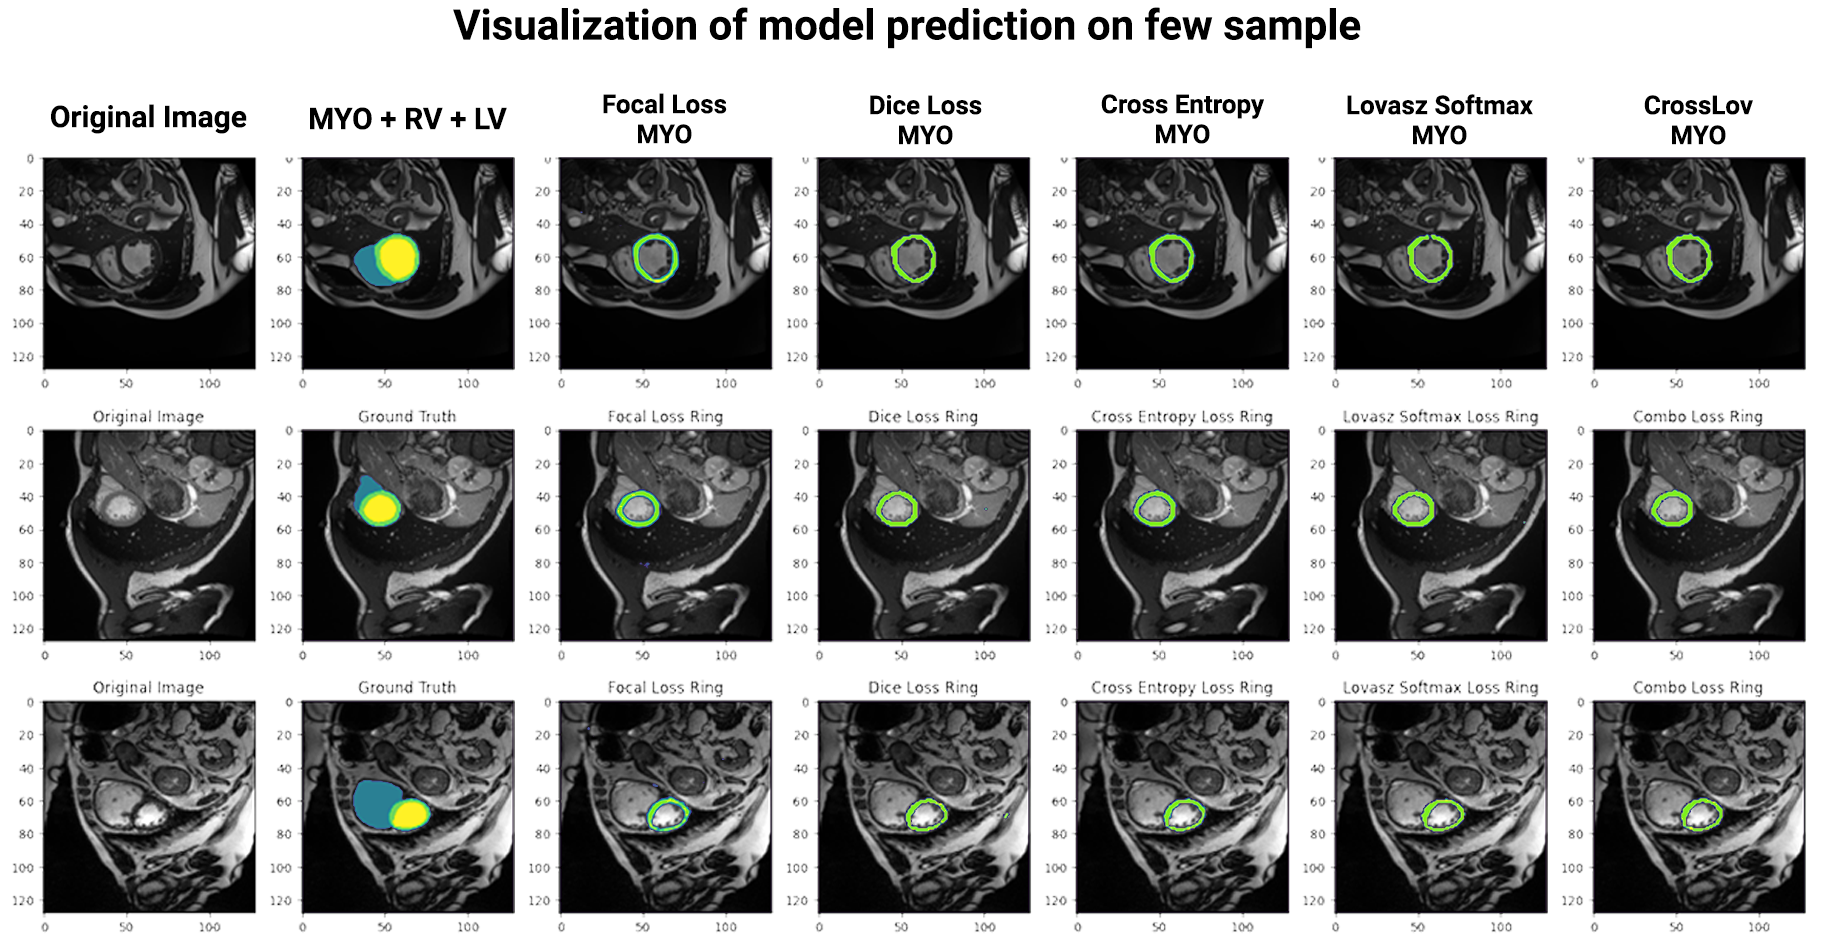
\includegraphics[width=0.86\textwidth]{bab5/ch5-visual-seg-analysis.png}
	\caption{Visual comparison of myocardium segmentation results obtained using the investigated loss functions. The predicted myocardium segmentation is shown in red, whereas the corresponding ground-truth annotation is shown in green \citep{Riandini2025Array}}
	\label{fig:ch5-visual-seg-analysis}
\end{figure}
\end{comment}

\begin{sidewaysfigure}[htbp]
	\centering
	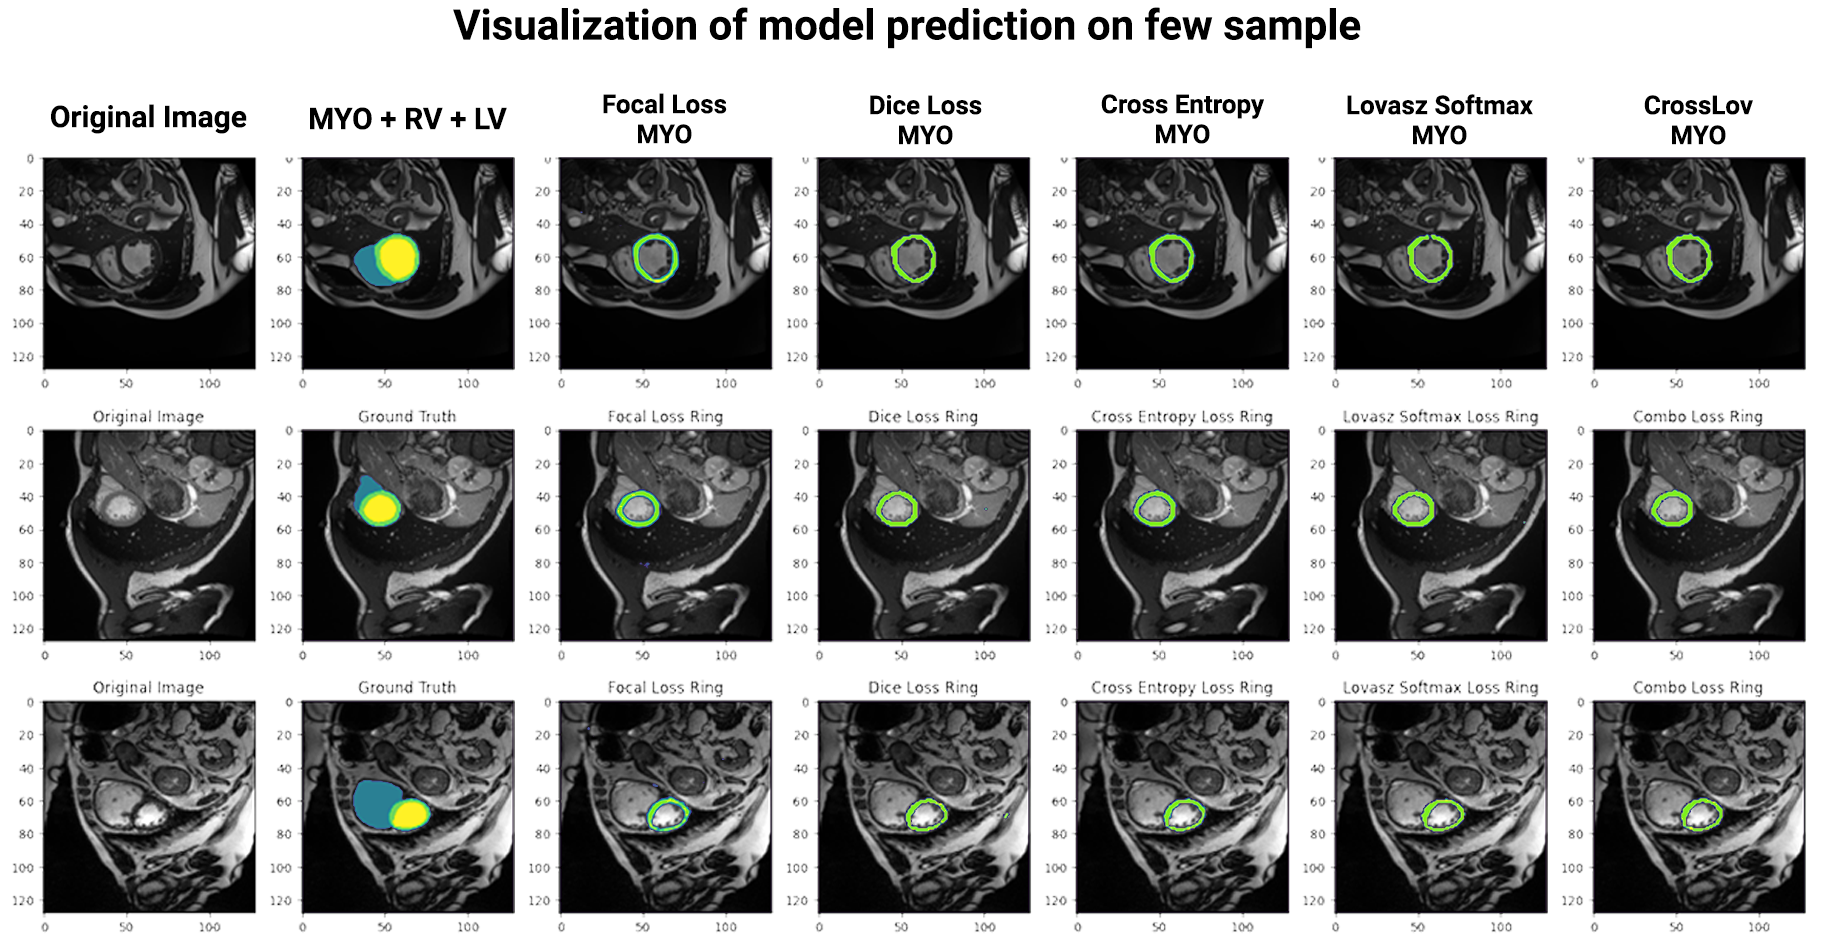
\includegraphics[width=\textwidth]{bab5/ch5-visual-seg-analysis.png}
	\caption{Visual comparison of myocardium segmentation results obtained using the investigated loss functions. The predicted myocardium segmentation is shown in red, whereas the corresponding ground-truth annotation is shown in green \protect\citep{Riandini2025Array}}
	\label{fig:ch5-visual-seg-analysis}
\end{sidewaysfigure}

As illustrated in Figure~\ref{fig:ch5-visual-seg-analysis}, all investigated loss functions successfully identified the myocardium region under identical experimental conditions. Nevertheless, noticeable differences can be observed in the continuity of the predicted myocardial contours and their agreement with the corresponding reference annotations. These visual differences demonstrate that the choice of optimization objective influences not only numerical evaluation metrics but also the anatomical appearance of the resulting segmentation masks.

The visual comparison indicates that \textbf{Cross-Entropy}, \textbf{Focal Loss}, and \textbf{Dice Loss} produced generally acceptable segmentation results but still exhibited visible discrepancies between the predicted contours and the reference annotations in several representative examples. Although these deviations are relatively small, they indicate that optimization based on a single learning objective may not consistently preserve both regional overlap and boundary accuracy.

In comparison, \textbf{Lovász-Softmax} generated segmentation masks that more closely followed the myocardial region, reflecting its superior regional overlap observed during the quantitative evaluation. This behaviour is consistent with the optimization objective of Lovász-Softmax, which directly promotes improved Intersection over Union (IoU) during network training. Consequently, the predicted myocardium contours demonstrate closer agreement with the reference annotation in terms of regional coverage.

Among the investigated approaches, \textbf{CrossLov} demonstrated the closest overall visual agreement with the corresponding ground-truth annotations. The predicted myocardial contours appear more continuous and more closely aligned with the anatomical boundaries of the reference segmentation, indicating improved consistency between overlap accuracy and boundary localization. These visual observations are consistent with the quantitative findings presented in the previous subsection, where CrossLov achieved the highest Dice Similarity Coefficient together with the lowest Hausdorff Distance among the investigated loss functions.

To facilitate interpretation of the qualitative observations presented in Figure~\ref{fig:ch5-visual-seg-analysis}, the principal visual findings are summarized in Table~\ref{tab:ch5-visual-assessment}.

\begin{table}[htbp]
	\centering
	\caption{Summary of visual assessment based on Figure 5.4}
	\label{tab:ch5-visual-assessment}
	
	\small
	\setlength{\heavyrulewidth}{\lightrulewidth}
	\renewcommand{\arraystretch}{1.3}
	\begin{tabularx}{\textwidth}{
			>{\raggedright\arraybackslash}p{0.22\textwidth}
			>{\raggedright\arraybackslash}X
			>{\raggedright\arraybackslash}X
		}
		\toprule
		\textbf{Loss Function} & \textbf{Visual Observation} & \textbf{Consistency with Quantitative Results} \\
		\midrule
		Cross-Entropy & Relatively consistent segmentation with minor discrepancies. & Consistent with moderate IoU and HD performance. \\ \addlinespace
		Focal Loss & Stable prediction but visible deviations in several samples. & Consistent with low training loss but moderate segmentation performance. \\ \addlinespace
		Dice Loss & Good regional overlap with several contour inconsistencies. & Consistent with competitive quantitative performance. \\ \addlinespace
		Lov\'asz-Softmax & Segmentation closely follows the myocardium region. & Consistent with the highest myocardium IoU. \\ \addlinespace
		CrossLov & Closest visual agreement with the reference annotation. & Consistent with the highest Dice Score and lowest HD. \\
		\bottomrule
	\end{tabularx}
\end{table}

The qualitative observations summarized in Table~\ref{tab:ch5-visual-assessment} demonstrate strong agreement with the quantitative evaluation presented in Section~\ref{subsec:ch5-quantitative-compare-loss}. The quantitative results are reflected in Dice Similarity Coefficient, Intersection over Union, and Hausdorff Distance are reflected in the visual appearance of the generated myocardium segmentation masks. In particular, the balanced quantitative performance achieved by CrossLov is accompanied by more consistent contour continuity and closer agreement with the reference annotations, whereas the strengths of Lovász-Softmax are primarily reflected in higher regional overlap.

Overall, the qualitative assessment confirms that the investigated loss functions influence not only quantitative segmentation accuracy but also the anatomical quality of the resulting myocardium segmentation. The consistency between the quantitative evaluation and the visual observations strengthens the reliability of the experimental findings and provides additional evidence that an appropriate optimization objective contributes substantially to accurate and anatomically consistent myocardium segmentation.

The findings obtained from the training behaviour analysis, quantitative evaluation, and qualitative visual assessment are integrated in the following section to provide a comprehensive discussion of the influence of the investigated loss functions on myocardium segmentation performance.

\begin{table}[htbp]
	\centering
	\caption{Summary of training behaviour}
	\label{tab:ch5-training-behaviour}
	
	\small
	\setlength{\heavyrulewidth}{\lightrulewidth}
	\renewcommand{\arraystretch}{1.3}
	\begin{tabularx}{\textwidth}{
			>{\raggedright\arraybackslash}p{0.45\textwidth}
			>{\raggedright\arraybackslash}X
		}
		\toprule
		\textbf{Observation} & \textbf{Result} \\
		\midrule
		Lowest Training Loss & Focal Loss (0.0012, Epoch 96) \\
		Lowest Testing Loss & Focal Loss (0.0011, Epoch 95) \\
		Highest Training Dice Score & CrossLov (98.266) \\
		Highest Testing Dice Score & CrossLov (98.099) \\
		Shortest Training Time & Cross-Entropy (5729.55 s) \\
		Longest Training Time & Focal Loss (6472 s) \\
		\bottomrule
	\end{tabularx}
\end{table}

\subsection{Overall Discussion}
\label{subsec:ch5-discussion}  

The experimental results presented throughout this chapter demonstrate that the selection of an appropriate loss function substantially influences myocardium segmentation performance, even when the segmentation architecture, preprocessing procedure, dataset partition, and training configuration remain unchanged. Since all comparative experiments employed an identical enhanced U-Net framework with fuzzy pooling, the observed differences in segmentation performance can be attributed exclusively to the investigated optimization objectives. These findings confirm that segmentation quality depends not only on the capability of the network architecture to extract representative image features but also on how the optimization objective guides the learning process during network training.

The training behaviour analysis presented in  Section~\ref{subsec:ch5-training-analysis} demonstrates that convergence of the optimization loss alone is insufficient to represent segmentation quality. Although \textbf{Focal Loss} consistently achieved the smallest training and testing loss values, it did not produce the highest segmentation accuracy according to the quantitative evaluation. Conversely, \textbf{CrossLov} achieved the highest Dice Similarity Coefficient despite not producing the lowest optimization loss. This observation indicates that minimizing the optimization objective does not necessarily maximize agreement between the predicted segmentation and the corresponding ground-truth annotation. Consequently, evaluating segmentation performance solely on the basis of convergence behaviour may lead to incomplete interpretation of model performance.

The quantitative evaluation further demonstrates that different optimization objectives emphasize different characteristics of myocardium segmentation. \textbf{Lovász-Softmax} achieved the highest Intersection over Union for myocardium segmentation, reflecting its capability to achieve higher regional overlap through direct optimization of an IoU-oriented objective. In contrast, \textbf{CrossLov} consistently achieved the highest Dice Similarity Coefficient together with the lowest Hausdorff Distance, indicating a more balanced capability to preserve both overlap accuracy and boundary consistency. The findings suggest that combining complementary optimization objectives provides a balanced trade-off between overlap accuracy and boundary localization.

The qualitative visual assessment further strengthens these findings. The segmentation masks generated using \textbf{CrossLov} demonstrated closer agreement with the reference annotations, exhibiting smoother myocardial contours and improved boundary continuity compared with the remaining investigated loss functions. Meanwhile, the segmentation masks produced by \textbf{Lovász-Softmax} reflected its superior regional overlap, whereas the remaining loss functions exhibited minor discrepancies that were consistent with their corresponding quantitative evaluation results. The agreement between the quantitative measurements and the qualitative observations increases confidence that the reported improvements represent genuine differences in segmentation performance rather than numerical variations alone.

To facilitate interpretation of the principal findings obtained throughout this comparative investigation, the overall experimental observations are summarized in Table~\ref{tab:ch5-overall-summary}.

\begin{table}[htbp]
	\centering
	\caption{Overall Summary of Experimental Findings}
	\label{tab:ch5-overall-summary}
	
	\small
	% Menyamakan ketebalan garis booktabs agar seragam tipis
	\setlength{\heavyrulewidth}{\lightrulewidth}
	% Memberikan padding vertikal yang lega
	\renewcommand{\arraystretch}{1.3}
	
	% \resizebox DIHAPUS agar font kembali ke ukuran normal/proporsional
	\begin{tabular}{ll}
		\toprule
		\textbf{Performance Aspect} & \textbf{Best-performing Loss Function} \\ \midrule
		Lowest Training Loss       & Focal Loss \\
		Lowest Testing Loss        & Focal Loss \\
		Shortest Training Time     & Cross-Entropy \\
		Highest Average IoU (MYO)  & Lov\'asz-Softmax \\
		Highest Dice Score         & CrossLov \\
		Lowest Average HD          & CrossLov \\ \bottomrule
	\end{tabular}
\end{table}

The summary presented in Table~\ref{tab:ch5-overall-summary} highlights that each investigated loss function contributes differently to myocardium segmentation performance. Rather than identifying a universally superior optimization objective, the comparative investigation demonstrates that individual loss functions emphasize different learning characteristics, including optimization convergence, computational efficiency, regional overlap, and boundary localization. Accordingly, selecting an appropriate loss function should consider the intended segmentation objective rather than relying exclusively on a single evaluation metric.

Among the investigated approaches, \textbf{CrossLov} consistently provided the most balanced overall performance by simultaneously achieving excellent overlap accuracy, accurate boundary localization, and competitive computational behaviour. These findings indicate that combining pixel-wise classification with region-based optimization enables the segmentation framework to generate more reliable and anatomically consistent myocardium representations than optimization strategies based on a single learning objective. Consequently, the results obtained in this chapter establish an improved myocardium segmentation framework that serves as a robust foundation for the residual attention-based myocardial scar segmentation framework developed in Chapter VI, where accurate myocardium segmentation is subsequently utilized to support scar segmentation and quantitative myocardial infarction assessment.

\section{Chapter Summary}
\label{sec:ch5-summary}  

This chapter systematically investigated the influence of different loss functions on myocardium ring segmentation using an identical enhanced U-Net architecture with fuzzy pooling. By isolating the loss function as the only experimental variable, the study demonstrated that different loss functions emphasize different aspects of segmentation performance. Among the evaluated approaches, CrossLov provided the most balanced overall performance, while Focal Loss achieved the lowest optimization loss, Cross-Entropy required the shortest training time, and Lovász-Softmax obtained the highest Intersection over Union. These findings were consistently supported by both quantitative and qualitative evaluations.

Overall, this chapter demonstrates that appropriate loss function selection plays an important role in achieving reliable myocardium segmentation. The findings provide a methodological basis for the myocardial scar assessment framework presented in Chapter VI, where accurate myocardium segmentation supports subsequent scar segmentation and quantitative scar area estimation.


		%\cleardoublepage
		\clearpage
		
		\chapter{RESIDUAL ATTENTION-BASED MYOCARDIAL SCAR SEGMENTATION AND QUANTIFICATION}

\label{chap:6}

\section{Overview}
\label{sec:ch6-intro-overview}

This chapter presents the final stage of the proposed deep learning framework for myocardial infarction assessment through residual attention-based myocardial scar segmentation and quantitative scar area assessment. Building upon the reliable anatomical myocardium representation established through the cardiac structure segmentation framework and loss function investigation presented in the previous chapters, this study focuses on identifying and quantifying myocardial scar tissue from multi-sequence cardiac magnetic resonance images to support objective myocardial infarction assessment.

Myocardial infarction (MI) causes irreversible myocardial injury that may subsequently lead to the formation of fibrotic scar tissue. The size and spatial distribution of myocardial scar are clinically relevant because they are associated with ventricular remodelling, impaired cardiac function, recurrent cardiac events, and patient prognosis. Therefore, accurate identification and quantitative assessment of myocardial scar constitute important components of CMR-based myocardial infarction analysis \citep{Richardson2015,Wu2021}.

Multi-sequence CMR provides complementary anatomical and pathological information by combining balanced Steady-State Free Precession (bSSFP), T2-weighted imaging (T2WI), and Late Gadolinium Enhancement (LGE). The bSSFP sequence primarily depicts cardiac anatomy, T2WI emphasizes myocardial oedema, whereas LGE provides high contrast for myocardial scar visualization. The spatial correspondence among these pre-aligned sequences enables complementary tissue characteristics to be jointly analysed, thereby providing a more comprehensive representation of myocardial pathology than any individual sequence alone \citep{Li2023MyoPS,Ding2023}.

Despite the availability of multi-sequence information, automated myocardial scar segmentation remains challenging. Scar regions are generally small, irregularly shaped, and heterogeneous in appearance. Their boundaries may also be difficult to distinguish from surrounding myocardial tissue. Conventional convolutional architectures may therefore fail to retain subtle pathological features or adequately emphasize the limited image regions associated with myocardial scar \citep{Wu2021}.

The investigations presented in Chapters IV and V established the anatomical foundation required for subsequent myocardial pathology analysis. Chapter IV developed an enhanced U-Net with fuzzy pooling for cardiac structure segmentation, whereas Chapter V investigated the influence of different loss functions on myocardium segmentation. Collectively, these investigations produced an improved myocardium representation that provides the anatomical basis for the myocardial scar analysis presented in this chapter.

To address the challenges associated with small, heterogeneous, and irregular myocardial scar regions, this chapter presents MyoScarNet-RA, a residual attention-based framework for myocardial scar segmentation and quantitative scar assessment. The proposed framework integrates residual learning and hybrid channel-spatial attention within a hierarchical encoder-decoder architecture. Residual connections facilitate effective information propagation through deep network layers, whereas the attention mechanism adaptively recalibrates channel and spatial feature responses to emphasize diagnostically relevant scar patterns while suppressing irrelevant background information \citep{He2016,Hu2018,Woo2018}.

The proposed framework does not terminate at pixel-wise segmentation. The predicted scar mask is further processed to estimate the physical scar area in square millimetres. This procedure enables segmentation output to be evaluated not only in terms of spatial correspondence with expert annotation but also through quantitative comparison between automated and manual scar area measurements \citep{Riandini2026Access}.

Accordingly, the objectives of this chapter are:

\begin{itemize}[nosep, leftmargin=*]
	\item to evaluate the capability of residual learning and hybrid attention for myocardial scar segmentation;
	\item to assess scar segmentation using overlap, boundary, and structural similarity measures;
	\item to estimate myocardial scar area from the predicted segmentation mask; and
	\item to evaluate the error, correlation, and agreement between automated scar area estimation and expert annotation.
\end{itemize}

The remainder of this chapter is organized as follows. Section~\ref{sec:ch6-framework} describes the proposed residual attention-based myocardial scar segmentation framework. Section~\ref{sec:ch6-materials} presents the dataset, image preparation, training configuration, reference architectures, and evaluation protocol. Section~\ref{sec:ch6-results} discusses the experimental results, including training behaviour, segmentation performance, scar area quantification, measurement agreement, and computational requirements. Section~\ref{sec:ch6-summary} summarizes the principal findings of the chapter.

\section{Proposed Residual Attention-Based Myocardial Scar Segmentation Framework}
\label{sec:ch6-framework}

The framework presented in this chapter extends the anatomical cardiac analysis established in Chapters IV and V toward automated myocardial scar segmentation and quantitative scar assessment. Rather than developing a completely independent segmentation pipeline, the proposed method builds upon the reliable myocardium representation obtained from the preceding investigations and focuses on identifying pathological scar tissue within multi-sequence CMR images. Using the proposed MyoScarNet-RA, the generated scar probability map is subsequently converted into a binary scar mask from which the physical scar area is estimated. Consequently, the framework integrates image segmentation and quantitative measurement into a unified analysis pipeline \citep{Riandini2026Access}.

\subsection{Overall Framework}
\label{subsec:ch6-overall}

The overall processing stages of the proposed framework are illustrated in Figure~\ref{fig:ch6-workflow}. The framework receives pre-aligned bSSFP, T2WI, and LGE images as complementary inputs. These images are prepared using the procedure described in Section~\ref{sec:ch6-materials} before being processed by the proposed residual attention network. The network generates a probability map representing the likelihood of scar presence at each pixel. The probability map is then converted into a binary scar mask, from which the scar area is calculated \citep{Li2023MyoPS,Riandini2026Access}.

\begin{figure}[htbp]
	\centering
	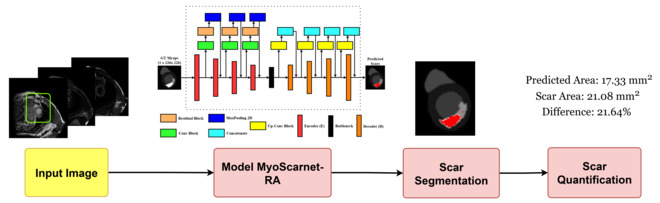
\includegraphics[width=\textwidth]{bab6/ch6-workflow.jpg}
	\caption{Overall workflow of the proposed myocardial scar segmentation and quantitative assessment framework \protect\citep{Riandini2026Access}}
	\label{fig:ch6-workflow}
\end{figure}

As shown in Figure~\ref{fig:ch6-workflow}, the framework consists of four sequential stages:

\begin{enumerate}[nosep, leftmargin=*]
	\item \textbf{Multi-sequence CMR input}, comprising spatially aligned bSSFP, T2WI, and LGE images.
	\item \textbf{Feature representation learning}, performed using residual blocks and hybrid channel-spatial attention.
	\item \textbf{Myocardial scar segmentation}, producing a pixel-wise scar probability map and binary scar mask.
	\item \textbf{Scar area quantification}, converting the segmented scar pixels into a physical area expressed in square millimetres.
\end{enumerate}

This sequential workflow establishes a direct dependency between scar segmentation and quantitative scar assessment. Since scar area estimation is computed directly from the segmented binary mask, inaccuracies in scar localization may propagate to the subsequent measurement stage. Consequently, reliable scar segmentation forms the computational foundation for accurate and reproducible myocardial scar quantification.

\subsection{MyoScarNet-RA Architecture}
\label{subsec:ch6-architecture}

MyoScarNet-RA is a single-stage hierarchical encoder-decoder network derived from the U-Net architecture for automated myocardial scar segmentation. The architecture integrates residual learning and hybrid channel-spatial attention to improve feature representation of small and heterogeneous scar regions while preserving efficient information propagation throughout the network. Residual blocks are incorporated throughout the encoder and decoder, whereas hybrid channel-spatial attention is applied at the bottleneck and after decoder feature fusion. The detailed architecture is shown in Figure~\ref{fig:ch6-architecture} \citep{Ronneberger2015,He2016,Riandini2026Access}.

\begin{figure}[htbp]
	\centering
	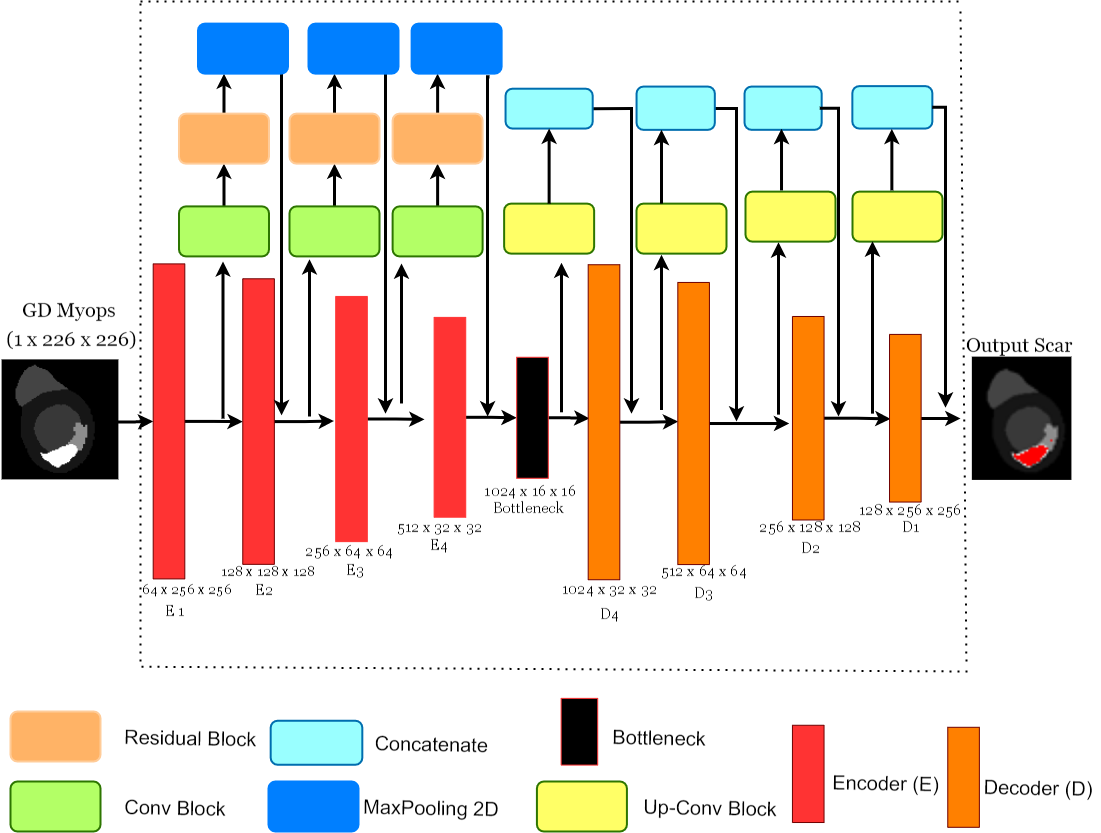
\includegraphics[width=\textwidth]{bab6/ch6-architecture.png}
	\caption{Architecture of the proposed MyoScarNet-RA for myocardial scar segmentation \protect\citep{Riandini2026Access}}
	\label{fig:ch6-architecture}
\end{figure}

As illustrated in Figure~\ref{fig:ch6-architecture}, feature extraction progresses through the encoder, information refinement is performed at the bottleneck using hybrid attention, and the decoder subsequently reconstructs the scar probability map through progressive feature fusion.

The architecture consists of three functional components:

\begin{itemize}[nosep, leftmargin=*]
	\item \textbf{Encoder}, responsible for extracting hierarchical image representations through four residual encoding stages;
	\item \textbf{Bottleneck}, responsible for refining the most abstract feature representation using residual learning and hybrid channel-spatial attention; and
	\item \textbf{Decoder}, responsible for reconstructing the final scar probability map through progressive feature fusion with skip connections.
\end{itemize}

The encoder consists of four stages, denoted as E1--E4. Each stage incorporates a residual block followed by max pooling. As the spatial resolution decreases, the number of feature channels increases, enabling the network to transform local intensity and texture information into more abstract representations of myocardial tissue and scar-related patterns. Residual connections are used to support information and gradient propagation through the deeper architecture \citep{He2016}.

At the bottleneck, a residual block is followed by hybrid channel-spatial attention. Channel attention assigns greater weight to feature channels containing relevant scar information, whereas spatial attention identifies image locations that are more likely to contain scar tissue. Their combination recalibrates the latent feature representation before spatial reconstruction begins \citep{Hu2018,Woo2018}.

The decoder comprises four stages, denoted as D4--D1. At each stage, the feature map is upsampled and concatenated with the corresponding encoder output. A residual block then refines the combined representation. Hybrid attention is applied following feature fusion so that the decoder can emphasize relevant scar characteristics at multiple spatial resolutions. A \(1 \times 1\)convolution followed by sigmoid activation produces the final probability map, with values ranging from zero to one \citep{Riandini2026Access}.

The complementary integration of residual learning and hybrid channel-spatial attention enables the proposed architecture to preserve efficient feature propagation while selectively emphasizing diagnostically relevant scar patterns. Consequently, the network learns both global contextual information and fine local scar characteristics, thereby improving feature representation of small and heterogeneous myocardial scar regions and supporting more accurate scar segmentation under complex myocardial tissue appearance \citep{He2016,Hu2018,Woo2018}.

The principal characteristics of MyoScarNet-RA can therefore be summarized as follows:

\begin{itemize}[nosep, leftmargin=*]
	\item
	residual blocks are used in both the encoder and decoder;
	\item
	hybrid channel-spatial attention is applied at the bottleneck and after decoder feature fusion;
	\item
	skip connections retain high-resolution spatial information;
	\item
	segmentation is completed in a single forward pass; and
	\item
	the network produces a pixel-wise scar probability map with an output resolution of $256 \times 256$ pixels.
\end{itemize}

\subsection{Myocardial Scar Segmentation}
\label{subsec:ch6-segmentation}

As illustrated in Figure~\ref{fig:ch6-architecture}, myocardial scar segmentation is performed through a single-stage encoder--decoder framework that transforms multi-sequence CMR images into a pixel-wise scar probability map. The three complementary CMR sequences are processed simultaneously to learn hierarchical feature representations describing both anatomical structures and pathological scar characteristics. These representations are progressively refined throughout the network before being reconstructed into the final segmentation output \citep{Riandini2026Access}.

During the forward propagation process, the encoder extracts increasingly abstract image features, while the bottleneck refines the latent representation through hybrid channel-spatial attention. The decoder subsequently restores spatial resolution by combining high-level semantic information with fine spatial features transferred through skip connections. This progressive reconstruction enables accurate localization of myocardial scar while preserving important anatomical details \citep{Ronneberger2015,Riandini2026Access}.

The final network output is a probability map, $P \in [0,1]^{H \times W}$, in which each pixel represents the estimated probability of belonging to the myocardial scar class. The probability map is subsequently converted into a binary scar mask using Otsu\textquotesingle s automatic thresholding procedure, as described in Section~\ref{subsec:ch6-area-method}. Because segmentation is completed within a single forward pass, the proposed framework does not require cascaded processing or an additional refinement network, thereby providing an efficient basis for subsequent quantitative scar area estimation \citep{Otsu1979,Riandini2026Access}.

\subsection{Myocardial Scar Area Quantification}
\label{subsec:ch6-area-method}

Following segmentation, the probability map produced by MyoScarNet-RA is converted into a binary scar mask using Otsu's automatic thresholding method. Otsu's method determines the threshold that maximizes the between-class variance of the pixel-value distribution, thereby separating scar and non-scar pixels without manual threshold selection \citep{Otsu1979}.

After thresholding, each non-zero pixel in the binary mask is interpreted as scar tissue. The total scar area is obtained by multiplying the number of scar pixels by the physical area represented by one pixel. This procedure is expressed as

\begin{equation}
	A_{\mathrm{scar}} = N_{\mathrm{scar}} \times R
	\label{eq:ch6-scar-area}
\end{equation}
where:
\begin{conditions}
	A_{\mathrm{scar}} & estimated myocardial scar area ($\text{mm}^2$); \\
	N_{\mathrm{scar}} & total number of non-zero pixels identified as scar tissue; and \\
	R & physical area represented by one image pixel ($\text{mm}^2/\text{pixel}$).
\end{conditions}

This formulation is consistent with the scar area quantification procedure implemented in Algorithm 2 of the source study, where scar size is calculated directly from the segmented binary mask \citep{Riandini2026Access}.

The complete quantification procedure adopted in this dissertation is summarized in Algorithm 6.1.

\begin{algorithm}[htbp]
	\caption{Automated Myocardial Scar Area Quantification}
	\label{alg:ch6-scar-quantification}
	\begin{algorithmic}[1]
		\Require Binary scar segmentation mask $M$, Pixel area $R$ ($\text{mm}^2$)
		\Ensure Estimated scar area $A_{\mathrm{scar}}$ ($\text{mm}^2$)
		\vspace{2pt}
		
		\State Convert the binary scar mask $M$ into a numerical array $M_{\mathrm{np}}$.
		\State Count the total number of scar pixels:
		\[
		N_{\mathrm{scar}} = \sum_{p \in M_{\mathrm{np}}} \mathbb{I}(p > 0)
		\]
		\Statex \hspace{\algorithmicindent} where $\mathbb{I}(\cdot)$ is the indicator function.
		\State Compute the scar area:
		\[
		A_{\mathrm{scar}} = N_{\mathrm{scar}} \times R
		\]
		\State \Return $A_{\mathrm{scar}}$
	\end{algorithmic}
\end{algorithm}

The estimated scar area is subsequently compared with the corresponding expert measurement. The quantitative evaluation includes absolute error, root mean square error, correlation analysis, and Bland--Altman agreement, which are presented in Section~\ref{sec:ch6-results}. The quantification procedure therefore provides a direct connection between the predicted scar mask and an interpretable physical measurement of scar extent.

\section{Materials and Experimental Setup}
\label{sec:ch6-materials}

The experiments presented in this chapter were conducted to evaluate the effectiveness of the proposed MyoScarNet-RA for myocardial scar segmentation and quantitative scar area estimation. To ensure a fair comparison, all evaluated models were implemented using identical dataset partitioning, preprocessing procedures, training configurations, and evaluation protocols. Consequently, any observed performance differences can be attributed primarily to architectural design rather than inconsistencies in the experimental protocol. The following subsections describe the dataset, image preparation, training configuration, and evaluation criteria adopted throughout the experimental study.

\subsection{MyoPS2020 Dataset}
\label{subsec:ch6-dataset}

The experiments were conducted using the \textbf{Myocardial Pathology Segmentation (MyoPS2020)} dataset, which contains pre-aligned multi-sequence CMR images together with expert annotations of myocardial pathology. Each subject includes three complementary imaging sequences, namely balanced Steady-State Free Precession (bSSFP), T2-weighted imaging (T2WI), and Late Gadolinium Enhancement (LGE). These three sequences provide complementary anatomical and pathological information that facilitates accurate myocardial scar segmentation \citep{Xue2020,Riandini2026Access}.

To avoid data leakage, dataset partitioning was performed at the patient level. Following the experimental protocol adopted in the source article, the dataset consisted of \textbf{36 patients for training (80\%)}, \textbf{5 patients for validation (11\%)}, and \textbf{4 patients for testing (9\%)}. This patient-wise partition ensures that images from the same subject are not simultaneously used for training and testing.




\begin{table}[h]
		\centering
		\caption{Dataset composition and patient-level splitting protocol} %\citep{Riandini2026Access}}
		\label{tab:ch6-partition}
		\begin{tabular}{lccc}
			\toprule
			\textbf{Set} & \textbf{Patients} & \textbf{Slices} & \textbf{Percentage} \\ \midrule
			Training     & 36                & 76              & 80\%       \\ 
			Validation   & 5                 & 15              & 11\%       \\ 
			Testing      & 4                 & 45              & 9\%        \\ \midrule
			\textbf{Total} & \textbf{45}     & \textbf{136}    & \textbf{100\%} \\ \bottomrule
		\end{tabular}
\end{table}
	


\begin{comment}
\begin{table}[htbp]
	\centering
	\fbox{\parbox{0.86\textwidth}{\centering Insert Patient-level dataset partition used throughout the experiments here}}
	\caption{Patient-level dataset partition used throughout the experiments \citep{Riandini2026Access}}
	\label{tab:ch6-partition}
\end{table}
%\noindent\textit{Source: Adapted from \citet{Riandini2026Access}.}
\end{comment}

The patient-wise data partition adopted in this study prevents images from the same subject from appearing in different subsets, thereby reducing the risk of information leakage during model development. This protocol enables a more reliable assessment of the proposed framework by ensuring that the reported performance reflects the ability of the network to generalize to previously unseen patients.

\subsection{Image Preparation and Training Configuration}
\label{subsec:ch6-preparation}

Image preparation followed the preprocessing procedure established in Chapter III to ensure methodological consistency throughout the dissertation. Briefly, all multi-sequence CMR images were resized to $256 \times 256$ pixels and subsequently normalized to reduce inter-image intensity variation. During training, data augmentation, including random horizontal flipping, image rotation, and image scaling, was applied to improve robustness against anatomical variability. The corresponding expert annotations were converted into binary scar masks and used as reference labels for supervised learning.

All experiments were implemented using the PyTorch deep learning framework under identical training settings for both the proposed model and the baseline architectures. A Dice-Cross Entropy loss function was applied during training using the Stochastic Gradient Descent (SGD) optimizer. The remaining implementation parameters, including batch size, learning-rate scheduling, and validation strategy, were maintained consistently throughout all experiments to ensure a fair comparison among the evaluated methods \citep{Riandini2026Access}.

\subsection{Reference Architectures and Evaluation Metrics}
\label{subsec:ch6-reference-models}

The effectiveness of the proposed MyoScarNet-RA was evaluated by comparison with two reference segmentation architectures, namely the \textbf{Simple U-Net} and the \textbf{Complex U-Net}. Both baseline models were trained using exactly the same dataset partition, preprocessing procedure, optimizer, and training configuration. Therefore, the comparative results reflect architectural differences rather than implementation bias.

Performance evaluation was conducted from both segmentation and quantitative assessment perspectives. Segmentation quality was assessed using the Dice Similarity Coefficient (DSC), Intersection over Union (IoU), Hausdorff Distance (HD), and Structural Similarity Index (SSIM). Quantitative scar estimation was subsequently evaluated using the Mean Absolute Error (MAE), Root Mean Square Error (RMSE), Pearson correlation coefficient, and Bland--Altman agreement analysis. Together, these complementary measurements provide a comprehensive evaluation of both segmentation accuracy and quantitative scar assessment capability \citep{Riandini2026Access}.

\section{Experimental Results and Discussion}
\label{sec:ch6-results}

\subsection{Training Behaviour Analysis}
\label{subsec:ch6-training}

The training behaviour of the proposed MyoScarNet-RA was first analysed to evaluate the convergence characteristics of the learning process before quantitative segmentation performance was assessed. Throughout training, both the training and validation datasets were monitored to examine whether the network learned representative myocardial scar features while maintaining stable generalization.

Figure~\ref{fig:ch6-training} illustrates the evolution of training accuracy and loss during the learning process.

\begin{figure}[htbp]
	\centering
	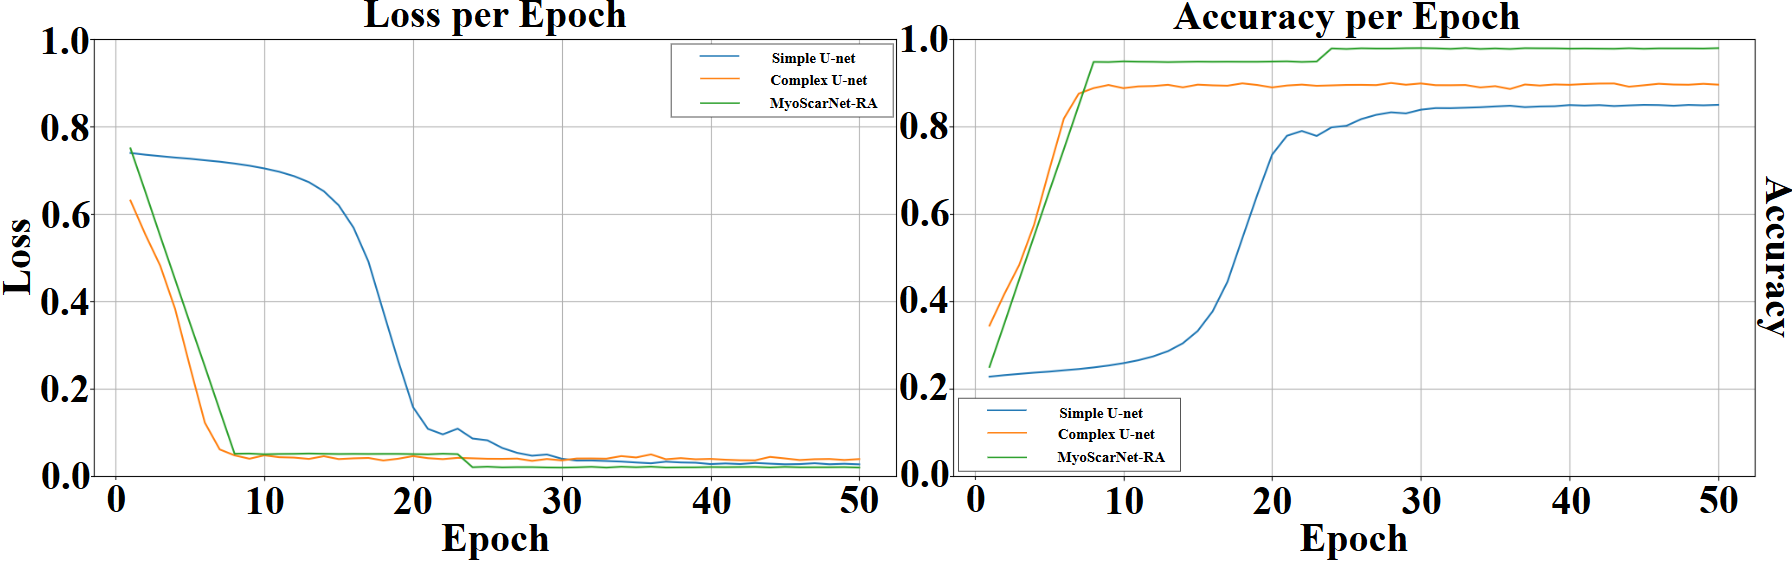
\includegraphics[width=\textwidth]{bab6/ch6-training.png}
	\caption{Training accuracy and loss curves of the proposed MyoScarNet-RA \protect\citep{Riandini2026Access}}
	\label{fig:ch6-training}
\end{figure}

\begin{comment}
\begin{figure}[htbp]
	\centering
	\fbox{\parbox{0.86\textwidth}{\centering Insert Training accuracy and loss curves of the proposed MyoScarNet-RA here}}
	\caption{Training accuracy and loss curves of the proposed MyoScarNet-RA \citep{Riandini2026Access}}
	\label{fig:ch6-training}
\end{figure}
%\noindent\textit{Source: Adapted from \citet{Riandini2026Access}.}
\end{comment}

As illustrated in Figure~\ref{fig:ch6-training}, the training accuracy increased progressively throughout the learning process, accompanied by a consistent reduction in both the training and validation losses. The similar trends exhibited by the two loss curves indicate that the proposed MyoScarNet-RA achieved stable learning behaviour without noticeable divergence between training and validation performance. This behaviour suggests that the network successfully learned representative myocardial scar features while maintaining satisfactory generalization to previously unseen validation samples.

Overall, the learning behaviour observed in Figure~\ref{fig:ch6-training} demonstrates that the adopted training configuration enabled stable model convergence before quantitative evaluation was performed. Establishing stable learning behaviour is important because the segmentation results presented in the following subsection should reflect the effectiveness of the proposed residual attention architecture rather than instability during network training.

\subsection{Scar Segmentation Performance}
\label{subsec:ch6-performance}

The segmentation performance of the proposed MyoScarNet-RA was quantitatively evaluated by comparison with the reference segmentation architectures under identical experimental conditions. The comparison employed four complementary performance measures, namely the Dice Similarity Coefficient (DSC), Intersection over Union (IoU), Hausdorff Distance (HD), and Structural Similarity Index (SSIM). Collectively, these metrics evaluate regional overlap, boundary accuracy, and structural similarity between the predicted scar segmentation and the corresponding expert annotation.

The quantitative comparison is presented in Table~\ref{tab:ch6-segmentation}, whereas representative segmentation examples are illustrated in Figure~\ref{fig:ch6-segmentation}.

\subsection{Scar Segmentation Performance}
\label{subsec:ch6-performance}

The segmentation performance of the proposed MyoScarNet-RA was quantitatively evaluated by comparison with the reference segmentation architectures under identical experimental conditions. The comparison employed six complementary performance measures, namely the Dice Similarity Coefficient (DSC), Intersection over Union (IoU), Hausdorff Distance (HD), Structural Similarity Index (SSIM), Sensitivity (SEN), and Specificity (SPE). Collectively, these metrics evaluate regional overlap, boundary accuracy, structural similarity, and voxel classification quality between the predicted scar segmentation and the corresponding expert annotation.

The quantitative comparison is presented in Table~\ref{tab:performance_comparison}, whereas representative segmentation examples are illustrated in Figure~\ref{fig:ch6-segmentation}.

\begin{table}[htbp]
	\centering
	\caption{Quantitative comparison of myocardial scar segmentation performance}
	\label{tab:performance_comparison}
	
	\small
	\setlength{\heavyrulewidth}{\lightrulewidth}
	\renewcommand{\arraystretch}{1.25} % Memberi ruang vertikal agar tidak terlalu rapat
	
	\begin{tabularx}{\textwidth}{
			>{\raggedright\arraybackslash}p{0.30\textwidth}
			>{\centering\arraybackslash}X
			>{\centering\arraybackslash}X
			>{\centering\arraybackslash}X
		}
		\toprule
		\textbf{Metric} & \textbf{Simple U-Net} & \textbf{Complex U-Net} & \textbf{MyoScarNet-RA} \\
		\midrule
		Residual (\cmark/\xmark) & \xmark & \cmark & \cmark \\
		Attention (\cmark/\xmark) & \xmark & \xmark & \cmark \\
		\midrule
		IoU & $0.8301 \pm 0.0875$ & $\mathbf{0.8880 \pm 0.0496}$ & $0.8758 \pm 0.0625$ \\
		HD (mm) & $11.45 \pm 10.44$ & $2.43 \pm 4.01$ & $\mathbf{1.31 \pm 0.53}$ \\
		Dice Score & $0.9047 \pm 0.0526$ & $0.9071 \pm 0.0279$ & $\mathbf{0.9326 \pm 0.0368}$ \\
		SSIM & $0.9132 \pm 0.0474$ & $\mathbf{0.9466 \pm 0.0241}$ & $0.9406 \pm 0.0301$ \\
		Sensitivity (SEN) & $\mathbf{0.9980 \pm 0.0025}$ & $0.9960 \pm 0.0065$ & $0.9795 \pm 0.0210$ \\
		Specificity (SPE) & $0.9992 \pm 0.0005$ & $0.9995 \pm 0.0003$ & $\mathbf{0.9996 \pm 0.0002}$ \\
		\bottomrule
		\multicolumn{4}{@{}p{\textwidth}@{}}{\vspace{4pt}\footnotesize 
			$^{\dagger}$ Values are reported as Mean $\pm$ SD evaluated on the MyoPS2020 dataset. \newline
			$^*$ HD = Hausdorff Distance; SSIM = Structural Similarity Index; SEN = Sensitivity; SPE = Specificity. Checkmarks (\cmark) indicate presence of architectural component; crosses (\xmark) indicate absence. Bold text indicates the best performance for each metric. \newline
			\textit{Source:} Adapted from \citet{Riandini2026Access}.}
	\end{tabularx}
\end{table}

\begin{comment}
\begin{table}[htbp]
	\centering
	\fbox{\parbox{0.86\textwidth}{\centering Insert quantitative comparison of myocardial scar segmentation performance here}}
	\caption{Quantitative comparison of myocardial scar segmentation performance \citep{Riandini2026Access}}
	\label{tab:ch6-segmentation}
\end{table}
%\noindent\textit{Source: Adapted from \citet{Riandini2026Access}.}
\end{comment}

As summarized in Table~\ref{tab:performance_comparison}, the proposed MyoScarNet-RA demonstrated highly competitive segmentation performance across all evaluated metrics. Although the Complex U-Net achieved the highest IoU ($0.8880 \pm 0.0496$) and SSIM ($0.9466 \pm 0.0241$), the proposed MyoScarNet-RA demonstrated the highest Dice score ($0.9326 \pm 0.0368$) and the best Hausdorff Distance ($1.3117 \pm 0.5287~\text{mm}$), indicating superior boundary localization accuracy. Furthermore, all evaluated models exhibited excellent specificity ($>0.999$) and high sensitivity ($>0.97$), confirming consistent background suppression and reliable scar identification across multi-sequence CMR images.


\begin{figure}[htbp]
	\centering
	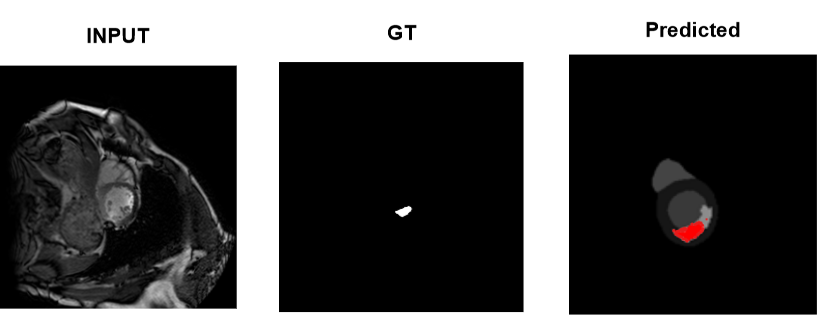
\includegraphics[width=\textwidth]{bab6/ch6-segmentation.png}
	\caption{Example of myocardial scar segmentation result obtained using the proposed MyoScarNet-RA \protect\citep{Riandini2026Access}}
	\label{fig:ch6-segmentation}
\end{figure}

The qualitative comparison presented in Figure~\ref{fig:ch6-segmentation} is consistent with these quantitative results. Relative to the Simple U-Net and Complex U-Net, the segmentation generated by MyoScarNet-RA follows the reference scar regions more consistently while reducing fragmented predictions and irregular boundary discontinuities. The improvement is particularly apparent in slices containing small and heterogeneous scar regions, where accurate localization is generally more challenging because of subtle intensity variation across the infarcted myocardium.

The observed segmentation performance can be attributed to the complementary interaction between residual learning and hybrid channel-spatial attention. Residual connections facilitate effective feature propagation throughout the network, whereas the attention mechanism selectively enhances diagnostically relevant scar features while suppressing irrelevant background responses. Consequently, the proposed architecture preserves both global contextual information and local scar characteristics, contributing to accurate boundary localization and reliable myocardial scar segmentation.


\subsection{Scar Area Quantification}
\label{subsec:ch6-area-results}

Following the evaluation of scar segmentation performance, the subsequent analysis investigates whether the generated segmentation masks can provide reliable quantitative scar measurements. Since the primary objective of the proposed framework is not only to identify scar tissue but also to estimate its physical extent, quantitative agreement between the automatically estimated scar area and the corresponding reference measurement becomes an essential indicator of the practical applicability of the proposed method.

The quantitative performance of the proposed scar area estimation was evaluated using the Mean Absolute Error (MAE), Root Mean Square Error (RMSE), and Pearson Correlation Coefficient (r). These complementary metrics respectively quantify the average estimation error, the magnitude of prediction deviation, and the degree of linear agreement between the automatically estimated scar area and the corresponding manual measurements performed by expert clinicians.

The evaluation metrics are formulated as follows:

\begin{equation}
	\mathrm{MAE}=\frac{1}{n}\sum_{i=1}^{n}\left|\hat{A}_{i}-A_{i}\right|
	\label{eq:ch6-mae}
\end{equation}

\begin{equation}
	\mathrm{RMSE}=\sqrt{\frac{1}{n}\sum_{i=1}^{n}\left(\hat{A}_{i}-A_{i}\right)^2}
	\label{eq:ch6-rmse}
\end{equation}

\begin{equation}
	r=\frac{\sum_{i=1}^{n}(\hat{A}_{i}-\overline{\hat{A}})(A_{i}-\overline{A})}{\sqrt{\sum_{i=1}^{n}(\hat{A}_{i}-\overline{\hat{A}})^2}\sqrt{\sum_{i=1}^{n}(A_{i}-\overline{A})^2}}
	\label{eq:ch6-pcc}
\end{equation}

where $\hat{A}_{i}$ and $A_i$ denote the automated and reference scar-area measurements for sample $i$, respectively, and $n$ is the number of evaluated samples.

The quantitative comparison between automated scar area estimation and manual measurement is summarized in Table~\ref{tab:ch6-area}. The proposed framework produced low estimation errors together with a strong linear relationship between the automatically estimated scar area and the corresponding expert measurements. These findings demonstrate that the proposed framework is capable of providing reliable scar area estimation, thereby providing a solid foundation for the agreement analysis presented in Section~\ref{subsec:ch6-agreement}.

\begin{comment}
	\begin{table}[htbp]
		\centering
		\fbox{\parbox{0.86\textwidth}{\centering Insert Quantitative evaluation of myocardial scar area estimation here}}
		\caption{Quantitative evaluation of myocardial scar area estimation \citep{Riandini2026Access}}
		\label{tab:ch6-area}
	\end{table}
	%\noindent\textit{Source: Adapted from \citet{Riandini2026Access}.}
\end{comment}

\begin{table}[htbp]
	\centering
	\caption{Scar area quantification: automated vs. manual annotation (our test split) \citep{Riandini2026Access}}
	\label{tab:ch6-area}
	
	\small
	\resizebox{\linewidth}{!}{%
		\begin{tabular}{lccc}
			\toprule
			\textbf{Image ID} & \textbf{Automated (mm$^2$)} & \textbf{Manual GT (mm$^2$)} & \textbf{Error (mm$^2$)} \\ \midrule
			117\_slice\_3 & 54.69 & 45.52 & +9.17 \\
			112\_slice\_3 & 29.00 & 24.16 & +4.84 \\
			107\_slice\_2 & 78.44 & 69.38 & +9.06 \\
			104\_slice\_0 & 65.69 & 52.60 & +13.09 \\
			120\_slice\_1 & 35.94 & 33.75 & +2.19 \\
			112\_slice\_0 & 16.62 & 16.77 & -0.15 \\
			119\_slice\_3 & 61.50 & 58.46 & +3.04 \\
			109\_slice\_0 & 20.06 & 16.46 & +3.60 \\
			121\_slice\_1 & 56.06 & 43.66 & +12.40 \\
			101\_slice\_3 & 48.62 & 41.04 & +7.58 \\
			103\_slice\_1 & 15.06 & 11.18 & +3.88 \\
			113\_slice\_0 & 26.00 & 20.56 & +5.44 \\
			116\_slice\_2 & 45.31 & 44.11 & +1.20 \\
			109\_slice\_1 & 41.56 & 35.37 & +6.19 \\
			122\_slice\_3 & 76.94 & 66.49 & +10.45 \\
			124\_slice\_2 & 52.44 & 46.49 & +5.95 \\ \bottomrule
		\end{tabular}%
	}
	
	\vspace{2mm}
	\begin{minipage}{\linewidth}
		\footnotesize
		\noindent $*$ Values are computed using our preprocessing and patient-level split; absolute errors can vary under different annotation protocols, slice selection rules, and data partitions.
	\end{minipage}
\end{table}

The representative examples presented in Figure~\ref{fig:ch6-area} visually demonstrate the capability of the proposed framework to estimate myocardial scar area across different infarction patterns. Despite variations in scar morphology, size, and spatial distribution, the estimated scar regions closely correspond to the manually annotated reference, indicating consistent preservation of scar extent and location. These visual observations are consistent with the quantitative results summarized in Table~\ref{tab:ch6-area} and further support the reliability of the proposed scar area estimation.

\begin{figure}[htbp]
	\centering
	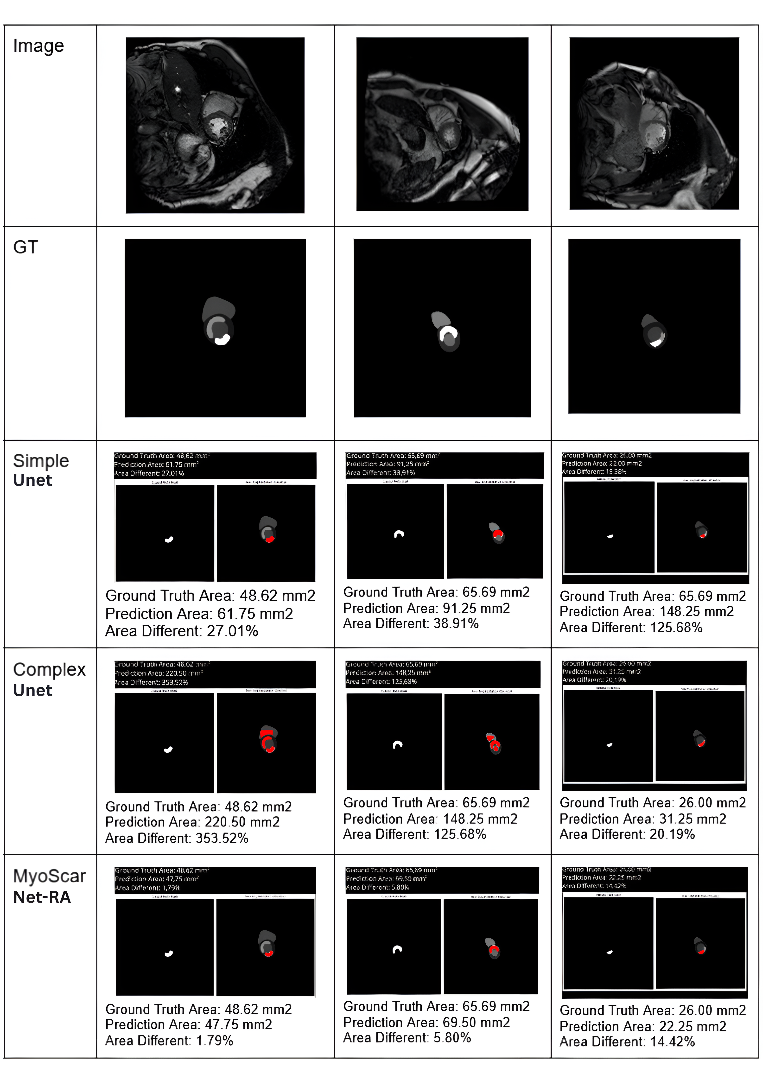
\includegraphics[width=\textwidth]{bab6/ch6-area.png}
	\caption{Representative examples of myocardial scar area estimation obtained using the proposed MyoScarNet-RA \protect\citep{Riandini2026Access}}
	\label{fig:ch6-area}
\end{figure}

The favourable quantitative performance observed in this study reflects the close relationship between scar segmentation accuracy and subsequent scar area estimation. Because scar area is calculated directly from the segmented scar mask, improvements in segmentation accuracy and reduction of boundary errors are translated into more reliable quantitative measurements. These findings indicate that accurate scar segmentation serves as the computational foundation for objective scar area estimation throughout the proposed framework.

Taken together, the quantitative results presented in Table~\ref{tab:ch6-area} and the representative examples shown in Figure~\ref{fig:ch6-area} demonstrate that accurate scar segmentation can be consistently translated into reliable physical scar area estimation, providing an objective representation of myocardial scar extent that complements conventional visual image interpretation.

From a clinical perspective, scar area quantification provides complementary information beyond visual interpretation alone. Rather than relying solely on qualitative visual assessment, clinicians are provided with an objective estimate of infarct extent that may support treatment planning, longitudinal patient follow-up, and evaluation of myocardial injury severity.

\subsection{Agreement Analysis}
\label{subsec:ch6-agreement}

Although the correlation analysis presented in the previous subsection demonstrates a strong linear relationship between automated and manual scar area measurements, correlation alone does not indicate whether the two measurement methods agree sufficiently for quantitative assessment. Therefore, Bland--Altman analysis was performed to evaluate the measurement agreement by analysing the distribution of estimation errors and identifying the presence of systematic measurement bias.

For each sample, the mean and difference between the automated and reference measurements are calculated as:
\begin{align}
	M_i &= \frac{\hat{A}_i + A_i}{2} \label{eq:ch6-ba-mean} \\
	D_i &= \hat{A}_i - A_i \label{eq:ch6-ba-difference}
\end{align}

The mean bias is:
\begin{equation}
	\overline{D} = \frac{1}{n} \sum_{i=1}^{n} D_i
	\label{eq:ch6-ba-bias}
\end{equation}

and the upper and lower 95\% limits of agreement are:
\begin{align}
	\mathrm{LoA}_{\mathrm{upper}} &= \overline{D} + 1.96 s_D \label{eq:ch6-ba-upper} \\
	\mathrm{LoA}_{\mathrm{lower}} &= \overline{D} - 1.96 s_D \label{eq:ch6-ba-lower}
\end{align}
where $s_D$ denotes the standard deviation of the measurement differences.

The agreement between automated and manual scar area measurements is illustrated in Figure~\ref{fig:ch6-bland-altman}.

\begin{comment}
\begin{figure}[htbp]
	\centering
	\fbox{\parbox{0.86\textwidth}{\centering Insert Bland--Altman plot comparing automated myocardial scar area estimation with expert measurements here}}
	\caption{Bland--Altman plot comparing automated myocardial scar area estimation with expert measurements \citep{Riandini2026Access}}
	\label{fig:ch6-bland-altman}
\end{figure}
%\noindent\textit{Source: Adapted from \citet{Riandini2026Access}.}
\end{comment}

\begin{figure}[htbp]
	\centering
	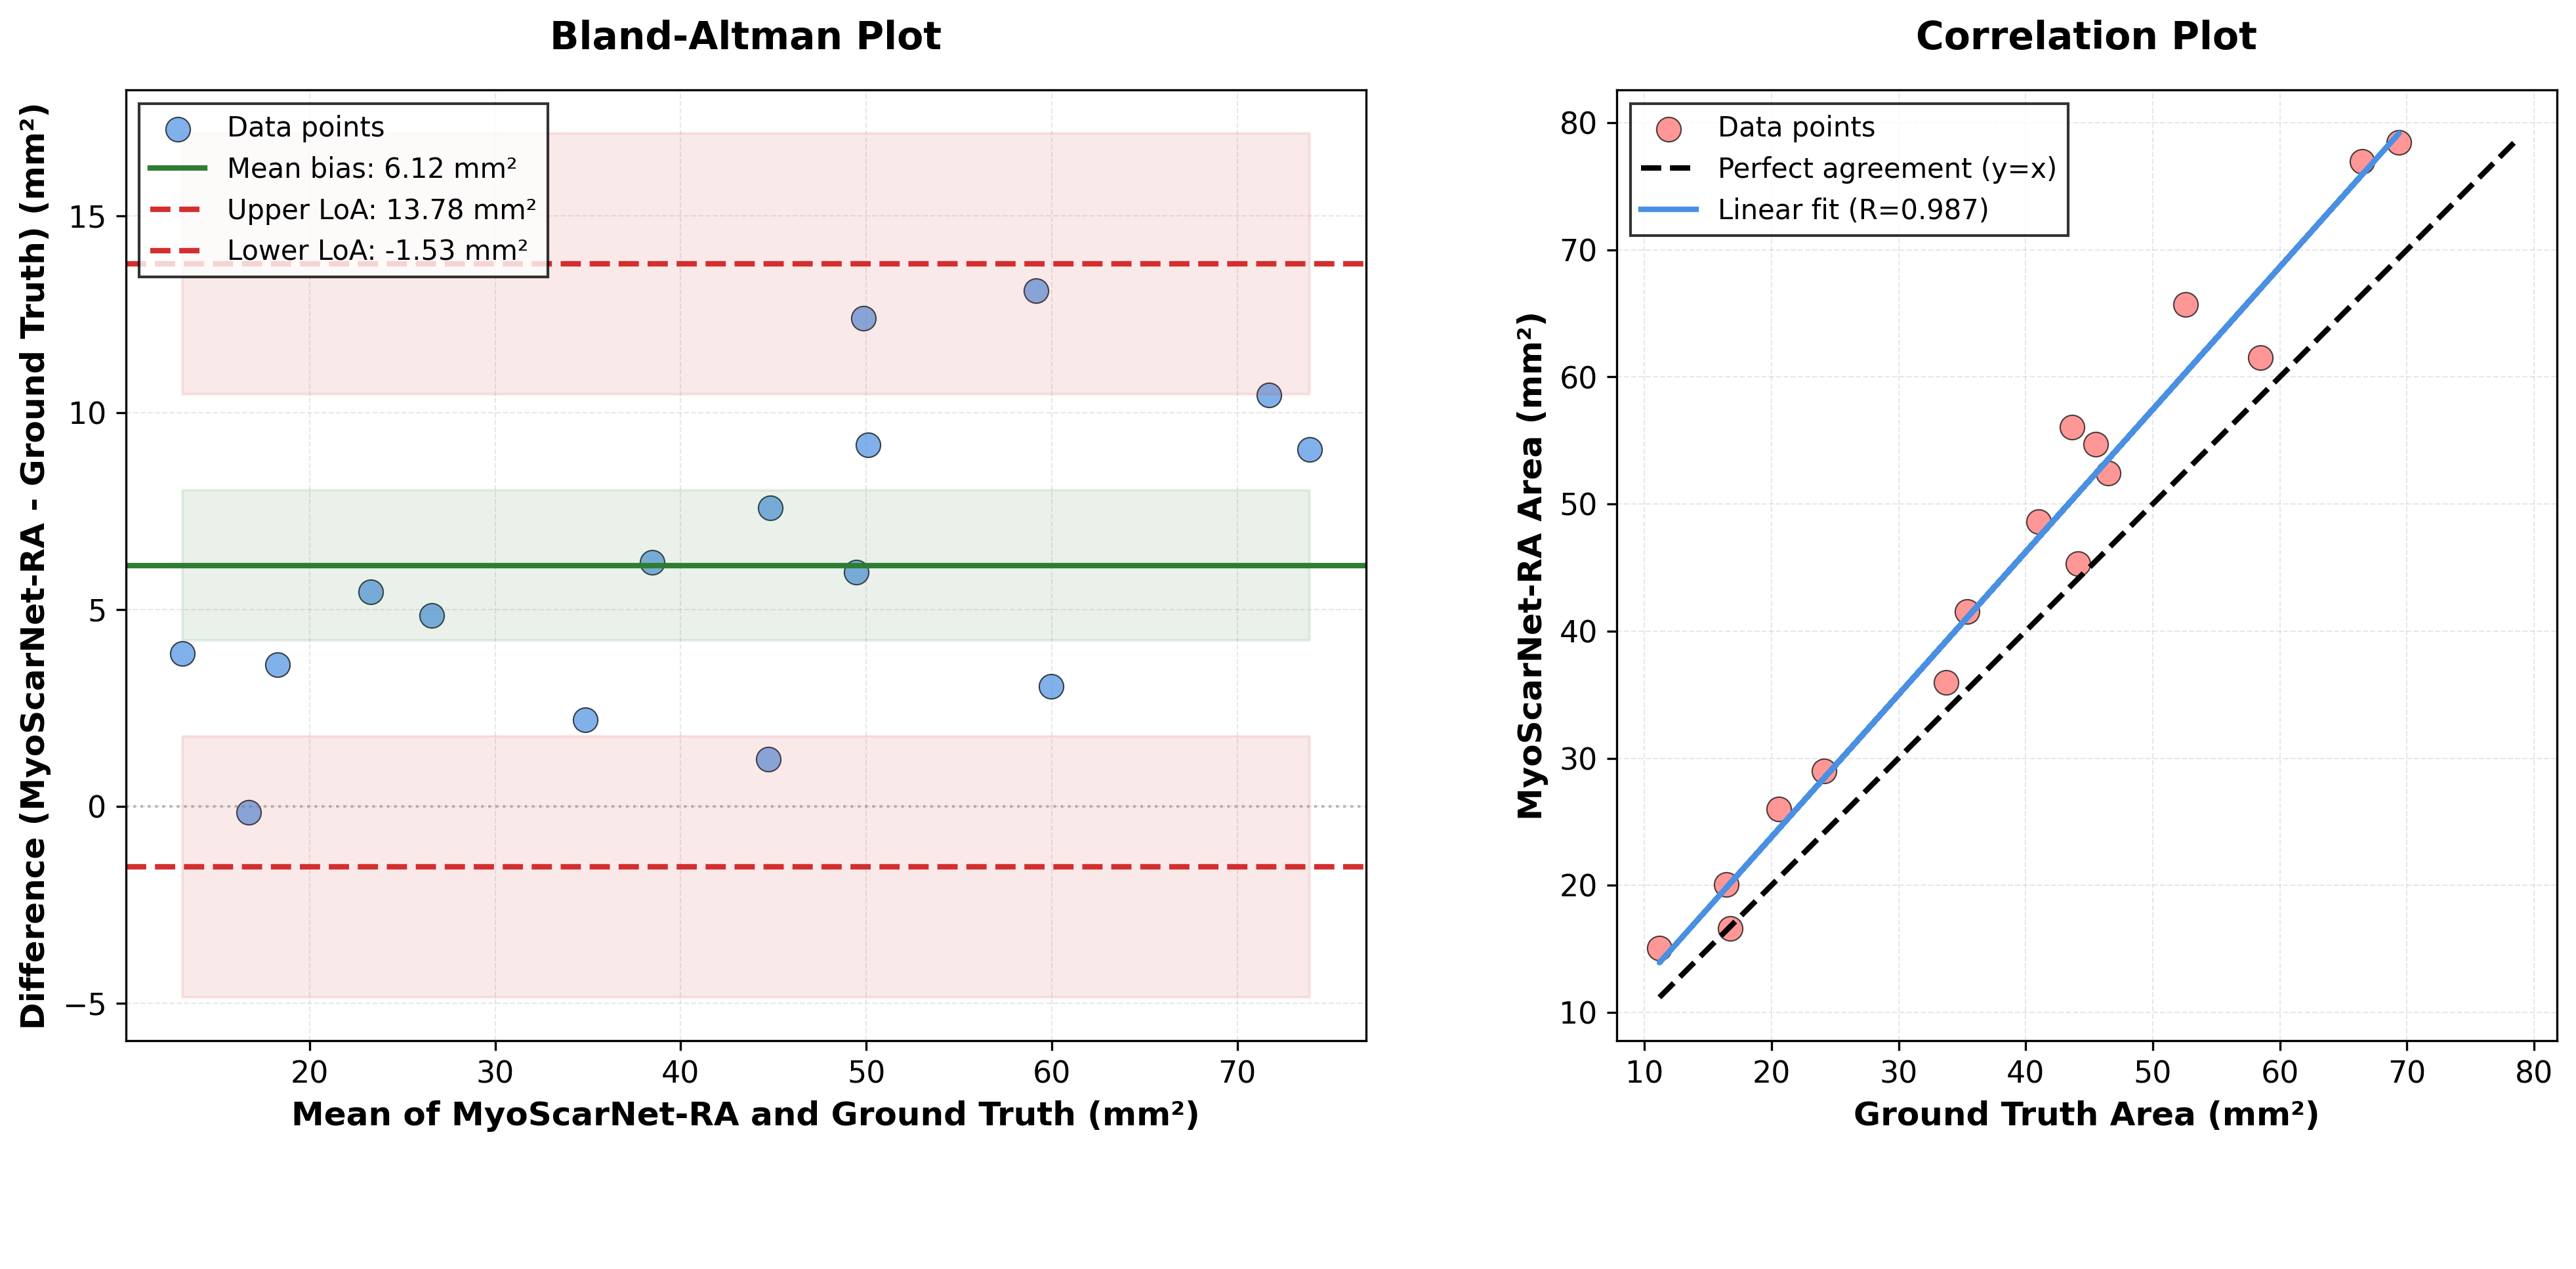
\includegraphics[width=\textwidth]{bab6/ch6-bland-altman.png}
	\caption{Bland--Altman plot analysis comparing automated myocardial scar area estimation with expert/manual measurements \protect\citep{Riandini2026Access}}
	\label{fig:ch6-bland-altman}
\end{figure}

As presented in Figure~\ref{fig:ch6-bland-altman}, the majority of measurement differences are distributed within the 95\% limits of agreement, indicating satisfactory agreement between the automated scar area estimation and the corresponding manual measurements. Only a limited number of observations are located near the agreement boundaries, suggesting that substantial estimation errors occur infrequently across the evaluated dataset.

The Bland--Altman analysis complements the correlation analysis presented in the previous subsection. While the Pearson correlation coefficient confirmed a strong linear relationship between automated and manual measurements, the Bland--Altman plot demonstrates that the differences between the two measurement methods remained relatively small and were randomly distributed around the mean bias. Together, these findings indicate that the proposed framework provides both a strong linear association and satisfactory agreement with expert measurements. These complementary agreement analyses demonstrate that the proposed scar quantification framework is capable of producing consistent quantitative measurements across the evaluated dataset.

From a clinical perspective, reliable measurement agreement is particularly important because myocardial scar area may influence patient risk stratification and treatment planning. The relatively small measurement bias obtained in this study suggests that the proposed framework can provide consistent quantitative scar estimation while maintaining close agreement with manual measurements performed by experienced observers. Consequently, the automated quantification procedure has the potential to reduce measurement variability and improve reproducibility without replacing expert clinical judgement.

\subsection{Computational Performance Analysis}
\label{subsec:ch6-computation}

In addition to segmentation accuracy and quantitative scar assessment, the computational characteristics of the proposed framework were also evaluated to determine its practical feasibility. Besides achieving high segmentation performance, a computer-aided myocardial scar analysis system should maintain computational requirements that remain compatible with routine deep learning implementation. Therefore, computational performance was assessed by considering both model complexity and inference efficiency.

The computational comparison between the proposed MyoScarNet-RA and the reference architectures is summarized in Table~\ref{tab:ch6-computation}.

\begin{table}[htbp]
	\centering
	\caption{Computational performance comparison of the evaluated segmentation frameworks}% \citep{Riandini2026Access}}
	\label{tab:ch6-computation}
	
	\small
	\resizebox{\linewidth}{!}{%
		\begin{tabular}{lccc}
			\toprule
			\textbf{Model} & \textbf{Avg. Time/Epoch (s)} & \textbf{Params} & \textbf{GPU Mem (GB)} \\ \midrule
			Simple U-Net   & $\mathbf{0.3684}$            & 7.76M           & 3.89                  \\
			Complex U-Net  & 1.5188                       & 31.04M          & 0.61                  \\
			\textbf{MyoScarNet-RA} & 2.1556                & 34.15M          & $\mathbf{0.40}$       \\ \midrule
			\textbf{Average:} & 1.3476                    & 18.30M          & 1.6367                \\ \bottomrule
		\end{tabular}%
	}
\end{table}

\begin{comment}
	\begin{table}[htbp]
		\centering
		\fbox{\parbox{0.86\textwidth}{\centering Insert computational performance comparison of the evaluated segmentation frameworks here}}
		\caption{Computational performance comparison of the evaluated segmentation frameworks \citep{Riandini2026Access}}
		\label{tab:ch6-computation}
	\end{table}
	%\noindent\textit{Source: Adapted from \citet{Riandini2026Access}.}
\end{comment}

As presented in Table~\ref{tab:ch6-computation}, incorporating residual learning and hybrid channel-spatial attention inevitably increased the architectural complexity compared with the conventional U-Net variants. Nevertheless, the proposed MyoScarNet-RA achieves the lowest GPU memory usage ($0.40~\text{GB}$) despite higher parameter count ($34.15\text{M}$) and computational time ($2.1556~\text{s/epoch}$), indicating efficiency in memory management while maintaining performance. These findings indicate that the additional computational cost is justified by the corresponding gain in analytical performance, resulting in a favourable balance between model complexity and segmentation capability.

Despite the inclusion of additional residual and attention modules, the proposed architecture maintained computational requirements that are compatible with contemporary GPU-based deep learning systems. This observation indicates that the improved segmentation performance was achieved without imposing excessive computational burden, thereby supporting the practical applicability of the proposed framework for automated myocardial scar analysis.

From the perspective of clinical implementation, computational efficiency is an important consideration because automated analysis should provide results within a reasonable processing time while maintaining high segmentation accuracy. The computational characteristics observed in this study demonstrate that the proposed MyoScarNet-RA satisfies these practical requirements by providing improved myocardial scar segmentation together with acceptable computational complexity.

\subsection{Overall Discussion}
\label{subsec:ch6-discussion}

The experimental results collectively demonstrate that the proposed MyoScarNet-RA provides a coherent framework for integrating myocardial scar segmentation with quantitative scar area estimation. The stable learning behaviour observed during training, together with the competitive segmentation performance and satisfactory quantitative agreement with expert measurements, indicates that the proposed architecture successfully preserves diagnostically relevant scar features throughout the complete analysis pipeline. Rather than evaluating segmentation and quantification as independent tasks, the present study demonstrates that accurate scar segmentation forms the computational basis for reliable quantitative scar assessment.

The complementary use of segmentation metrics, quantitative error measurements, correlation analysis, and Bland--Altman agreement provides a comprehensive evaluation of the proposed framework from multiple perspectives. Rather than relying on a single performance indicator, these analyses collectively demonstrate that the predicted scar masks preserve sufficient anatomical information for subsequent quantitative assessment. Consequently, the proposed framework extends conventional image segmentation toward objective myocardial scar quantification that may assist clinical interpretation.

Despite these encouraging findings, several limitations should be acknowledged. The proposed framework was evaluated using the MyoPS2020 dataset, and its generalization to larger multi-centre datasets remains to be investigated. In addition, the present study focused exclusively on myocardial scar segmentation and scar area quantification without incorporating clinical outcome prediction or prognostic analysis. These aspects provide opportunities for future research aimed at extending the applicability of the proposed framework while preserving the anatomical foundation established throughout this dissertation.

Overall, this chapter demonstrates that the proposed MyoScarNet-RA effectively extends anatomical myocardium segmentation toward automated myocardial scar segmentation and quantitative scar assessment. Together with the investigations presented in Chapters IV and V, the present study establishes a coherent deep learning-based framework for CMR image analysis, beginning with anatomical cardiac structure segmentation, followed by improved myocardium segmentation through loss function investigation, and culminating in automated myocardial scar segmentation and quantitative scar assessment. Collectively, these contributions establish an integrated framework for objective myocardial infarction analysis using CMR.

\section{Chapter Summary}
\label{sec:ch6-summary}

This chapter presented MyoScarNet-RA, a residual attention-based framework for automated myocardial scar segmentation and quantitative scar area assessment using multi-sequence CMR images. Building upon the reliable myocardium segmentation established in Chapter V, the proposed framework enabled accurate myocardial scar segmentation and scar area estimation.

Experimental results demonstrated that the proposed framework supports CMR-based myocardial scar assessment. Together with the investigations presented in Chapters IV and V, this chapter completes the proposed deep learning framework developed in this dissertation. The following chapter presents the overall conclusions, scientific contributions, study limitations, and future research directions.

		%\cleardoublepage
		\clearpage
		
		\chapter{CONCLUSIONS AND FUTURE WORKS}
\label{chap:7}

\section{Conclusions}
\label{sec:ch7-conclusions}

\subsection{Contribution to Cardiac Structure Segmentation}

The first contribution of this research is the development of an enhanced U-Net framework incorporating fuzzy pooling for automatic cardiac structure segmentation from cine Cardiac Magnetic Resonance (CMR) images. The proposed framework demonstrated that replacing conventional pooling operations with fuzzy pooling improves feature preservation during the encoding process while maintaining computational efficiency. Experimental evaluation using the ACDC dataset confirmed that the proposed framework achieved accurate segmentation of the left ventricle, right ventricle, and myocardium, providing a reliable anatomical representation that serves as the foundation for subsequent myocardium and myocardial scar analysis.

\subsection{Contribution to Myocardium Segmentation}

The second contribution of this research is the systematic investigation of different loss functions for reliable myocardium segmentation using an identical segmentation framework. By maintaining the same network architecture, dataset, preprocessing procedure, and experimental configuration throughout all comparative experiments, the influence of the loss function was evaluated independently. The experimental results demonstrated that different loss functions emphasize different aspects of segmentation performance. Among the investigated approaches, CrossLov consistently provided the most balanced segmentation performance by simultaneously achieving high overlap accuracy and accurate boundary localization. These findings demonstrate that appropriate loss function selection plays an important role in achieving reliable and anatomically consistent myocardium segmentation.

\subsection{Contribution to Myocardial Scar Assessment}

The third contribution of this research is the development of the MyoScarNet-RA framework for automated myocardial scar assessment from multi-sequence CMR images. By integrating residual learning with a hybrid attention mechanism, the proposed framework effectively captures both local structural details and contextual contextual information required for accurate scar segmentation and quantitative scar area estimation. Experimental evaluation demonstrated that the proposed framework achieved reliable scar segmentation and quantitative scar assessment, providing an effective approach for automated analysis of myocardial infarction-related scar characteristics from CMR images.

\subsection{Overall Scientific Contribution}
\label{subsec:ch7-scientific-contributions}

This dissertation presents an integrated deep learning framework for cardiac magnetic resonance image analysis toward myocardial infarction assessment by systematically addressing three complementary stages, namely cardiac structure segmentation, myocardium segmentation, and myocardial scar assessment. Collectively, the proposed methods demonstrate that reliable CMR image analysis benefits from the integration of accurate anatomical representation, appropriate loss function selection, and robust myocardial scar assessment. These complementary contributions establish a coherent methodological framework and represent an important step toward automated myocardial infarction assessment.

\section{Limitations}
\label{sec:ch7-limitations}

This research has several limitations that should be acknowledged. First, the proposed methods were evaluated using publicly available benchmark datasets, which may not fully represent the diversity of clinical imaging protocols, scanner vendors, and patient populations encountered in real-world practice. Second, each methodological contribution was developed and evaluated independently to investigate specific research objectives rather than as a unified end-to-end framework. Third, the scope of myocardial scar assessment was limited to automated scar segmentation and quantitative scar area estimation, without incorporating additional clinical indicators or patient outcome analysis.

Despite these limitations, the proposed methods provide complementary methodological contributions that collectively establish a coherent framework for cardiac magnetic resonance image analysis toward myocardial infarction assessment.

\section{Future Works}
\label{sec:ch7-future-work}

Building upon the contributions of this dissertation, several directions for future research can be explored. First, the proposed framework should be validated using larger multi-center CMR datasets acquired from different institutions and MRI vendors to further evaluate its robustness and generalization capability under diverse clinical imaging conditions.

Second, future studies may investigate an end-to-end deep learning framework that integrates cardiac structure segmentation, myocardium segmentation, and myocardial scar assessment within a unified learning architecture. Such an approach may improve computational efficiency while enhancing consistency across different stages of the analysis pipeline.

Third, additional quantitative imaging biomarkers, such as scar transmurality, myocardial tissue characteristics, and ventricular functional parameters, may be incorporated to provide a more comprehensive assessment of myocardial infarction from CMR images.

Finally, prospective clinical validation involving collaboration with cardiologists is required to evaluate the applicability of the proposed framework in routine clinical practice and to further support the development of automated CMR-based myocardial infarction assessment.
		%\cleardoublepage
		\clearpage
		
	\end{spacing}
	
	\DaftarPustaka
	
	\DaftarRiwayatHidup
\end{document}